\PassOptionsToPackage{table}{xcolor}
\documentclass[11pt,twoside]{article}

\usepackage[margin=1in]{geometry}
\usepackage[T1]{fontenc}
\usepackage{lmodern}
\usepackage[utf8]{inputenc}
\usepackage{microtype}
\usepackage{xcolor}
\usepackage{setspace}
\definecolor{headergray}{gray}{0.50}
\definecolor{footgray}{gray}{0.50}
\definecolor{tableheaderbg}{gray}{0.82}
\definecolor{tablerowbg}{gray}{0.94}
\usepackage{amsmath,amssymb,amsthm,mathtools}
\usepackage{enumitem}
\usepackage{booktabs}
\usepackage{array}
\usepackage{caption}
\usepackage{tikz}
\usetikzlibrary{arrows.meta,positioning,calc,fit,backgrounds,decorations.pathreplacing}
\usepackage[colorlinks=true,linkcolor=blue,citecolor=blue,urlcolor=blue]{hyperref}
\usepackage[nameinlink,noabbrev]{cleveref}
\usepackage{csquotes}
\usepackage[backend=biber,style=alphabetic,sorting=nyt,maxbibnames=99]{biblatex}
\addbibresource{observer_geometry_1.refs.bib}
\usepackage{fancyhdr}
\usepackage{lastpage}
\usepackage{etoolbox}

\hypersetup{
  pdftitle={Observer Geometry I: Beyond Distance – Projection, Basis, Accumulation, and Observer Signatures},
  pdfauthor={James Ross},
  pdfpagelayout=SinglePage,
  pdfdirection=L2R
}

% Typography controls for publication-style pagination.
\clubpenalty=10000
\widowpenalty=10000
\displaywidowpenalty=10000
\brokenpenalty=10000
\interfootnotelinepenalty=10000
\doublehyphendemerits=100000
\finalhyphendemerits=1000000
\emergencystretch=2em
\raggedbottom
\setstretch{1.12}
\setlength{\parindent}{0pt}
\setlength{\parskip}{0.72em}

\captionsetup[figure]{font=small,labelfont=bf,textfont=it}
\captionsetup[table]{font={small},labelfont=bf}
\newcommand{\TableHeaderRow}{\rowcolor{tableheaderbg}\bfseries}
\AtBeginEnvironment{table}{\rowcolors{2}{tablerowbg}{white}}
\AtEndEnvironment{table}{\rowcolors{2}{}{}}

\setlength{\headheight}{30pt}
\newcommand{\paperdoi}{DOI: 10.5281/zenodo.18868896}
\newcommand{\paperversion}{Version 1.0.0}
\newcommand{\publicationdate}{March 5, 2026}
\newcommand{\runningauthor}{James Ross}
\newcommand{\runningtitle}{Observer Geometry I: Beyond Distance}

\fancypagestyle{ogmain}{%
  \fancyhf{}
  \fancyhead[C]{\footnotesize \textcolor{headergray}{\runningtitle}}
  \fancyfoot[R]{\footnotesize \textcolor{footgray}{\thepage\ of \pageref*{LastPage}}}
  \renewcommand{\headrulewidth}{0pt}
  \renewcommand{\footrulewidth}{0pt}
}

\fancypagestyle{ogtitle}{%
  \fancyhf{}
  \fancyfoot[C]{\tiny Copyright \textcopyright\ 2026 James Ross. Licensed under the \href{https://creativecommons.org/licenses/by/4.0/}{Creative Commons Attribution 4.0 International License}.}
  \fancyfoot[R]{\footnotesize \textcolor{footgray}{\thepage\ of \pageref*{LastPage}}}
  \renewcommand{\headrulewidth}{0pt}
  \renewcommand{\footrulewidth}{0pt}
}

\fancypagestyle{plain}{%
  \fancyhf{}
  \fancyhead[C]{\footnotesize \textcolor{headergray}{\runningtitle}}
  \fancyfoot[R]{\footnotesize \textcolor{footgray}{\thepage\ of \pageref*{LastPage}}}
  \renewcommand{\headrulewidth}{0pt}
  \renewcommand{\footrulewidth}{0pt}
}

\pagestyle{ogmain}
% Start each major section on a new page.
\pretocmd{\section}{\clearpage}{}{}

\newtheorem{theorem}{Theorem}[section]
\newtheorem{proposition}[theorem]{Proposition}
\newtheorem{lemma}[theorem]{Lemma}
\newtheorem{corollary}[theorem]{Corollary}
\theoremstyle{definition}
\newtheorem{definition}[theorem]{Definition}
\newtheorem{remark}[theorem]{Remark}

\newcommand{\Hist}{\mathbf{Hist}}
\newcommand{\Tr}{\mathbf{Tr}}
\newcommand{\proj}{\mathrm{proj}}
\newcommand{\basis}{\mathrm{basis}}
\newcommand{\acc}{\mathrm{acc}}
\newcommand{\task}{\mathrm{task}}
\newcommand{\blue}{\mathrm{blue}}
\newcommand{\red}{\mathrm{red}}
\newcommand{\good}{\mathrm{good}}
\newcommand{\bad}{\mathrm{bad}}
\newcommand{\bulk}{\mathrm{bulk}}
\newcommand{\conf}{\mathrm{conf}}
\newcommand{\TaskBundle}{\mathbb{T}}
\newcommand{\AION}{AI\ensuremath{\Omega}N}
\newcommand{\paperkeywords}{observer geometry; rulial distance; projection; basis; accumulation; observer signatures; degeneracy; structural insufficiency; bias gap}
\newcommand{\paperabstract}{Observers can agree on terminal state while disagreeing on conflict history, intent preservation, or replayability. These cases show that scalar comparison alone is insufficient for observer analysis. This paper inaugurates the Observer Geometry Series (OG-I), derived from the \AION\ Foundation Series (WARP~I--V), where budgeted observer geometry was introduced in WARP~IV. Translation cost remains essential but incomplete: observers may be state-close yet provenance-far, extensionally aligned yet conflict-structurally distinct, or equivalent at unbounded resources while sharply separated at finite budgets. We therefore model an observer as a projection equipped with a native basis and, when relevant, an accumulation process over prefixes. On this foundation, we define aperture, degeneracy, task-conditioned degeneracy, structural insufficiency floors, bias gaps, multi-component observer signatures, and budget elasticity. We prove coarsening monotonicity results and separation theorems showing that observer dominance does not admit exact scalar collapse in general, and we provide finite witness constructions for state/provenance separation, task sufficiency without historical faithfulness, and accumulation-level separation under equal projection and basis. The resulting framework extends observer geometry from translation cost alone to a calculus of visibility, ambiguity, recoverability, and task-relative correctness.}
\DeclareMathOperator{\BiasGap}{BiasGap}
\DeclareMathOperator{\Dist}{Dist}
\DeclareMathOperator{\Mor}{Mor}
\DeclareMathOperator{\cod}{cod}


\tikzset{
  ogbox/.style={draw=black, rounded corners=2pt, line width=0.9pt, fill=white, align=center, inner sep=6pt},
  ogaltbox/.style={draw=black, rounded corners=2pt, line width=0.9pt, fill=white, align=center, inner sep=6pt},
  ogwarnbox/.style={draw=black, rounded corners=2pt, line width=0.9pt, fill=white, align=center, inner sep=6pt},
  ogline/.style={-{Latex[length=2.7mm,width=2mm]}, line width=0.9pt},
  ogthin/.style={-{Latex[length=2mm,width=1.5mm]}, line width=0.7pt}
}

\title{Observer Geometry I: Beyond Distance\\\large Projection, Basis, Accumulation, and Observer Signatures}
\author{}
\date{}

\begin{document}

\begingroup
\thispagestyle{ogtitle}
\begin{center}
\vspace*{-0.03\textheight}
{\fontsize{28}{32}\selectfont\bfseries\fontseries{bx}\selectfont Observer Geometry I\par}
{\fontsize{24}{28}\selectfont\bfseries\fontseries{bx} Beyond Distance\par}
\vspace{0.20em}
{\Large\bfseries Projection, Basis, Accumulation, and Observer Signatures\par}
\vspace{0.18em}
{\normalsize \paperdoi\\[-0.22em]}
{\normalsize \paperversion\quad \publicationdate\par}
\vspace{0.48em}
{\large James Ross\\[-0.14em]}
{\normalsize Independent Researcher\\[-0.14em]}
{\normalsize ORCID: 0009-0006-0025-7801\\[-0.14em]}
{\normalsize \href{mailto:james@flyingrobots.dev}{\texttt{james@flyingrobots.dev}}\par}
\vspace{0.85em}
\begin{minipage}{0.8\textwidth}
\small
\textbf{Abstract.} \paperabstract
\par
\vspace{1.25em}
\textbf{Keywords.} \textit{\paperkeywords}
\end{minipage}
\end{center}
\endgroup
\clearpage

\begingroup
\setstretch{0.96}
\setlength{\parskip}{0pt}
\tableofcontents
\endgroup

\section{Introduction}
\label{sec:intro}

We begin with a motivating contrast. Two replicas can end in the same visible state, \(\mathrm{color}=\blue\), while arising from different histories: one with a single blue write and one with a red/blue conflict silently merged to blue. A state-only observer identifies these histories, whereas a provenance-aware observer separates them. We analyze when agreement on visible output constitutes genuine observer agreement and when it masks causal loss.

In this paper, we initiate the Observer Geometry Series as an independent line derived from the \AION\ Foundation Series (WARP~I--V). WARP~I--II establish deterministic rewriting state semantics~\cite{ross_paper_i,ross_paper_ii}; WARP~III adds provenance payloads and replay structure~\cite{ross_paper_iii}; WARP~IV introduces budgeted observer translation geometry~\cite{ross_paper_iv}; WARP~V shows that observer-level coarse-graining changes effective rulial dynamics~\cite{ross_paper_v}.

We proceed from a single claim: scalar distance is necessary but not sufficient. Translation cost captures one axis of comparison, but omits others. Observers can be state-close yet provenance-far, extensionally aligned yet intent-divergent, or equivalent at unbounded resources while sharply separated at finite budgets.

To formalize this claim, we model a structural observer as
\[
  S=(O,\mathcal{B}_S,M_S,K_S,E_S),
\]
where \(O\) is projection, \(\mathcal{B}_S\) is native basis, and \((M_S,K_S,E_S)\) is accumulation/emission structure. Projection captures what is seen, basis what is natively expressible, and accumulation what can be built over time.

Task error is defined only after fixing a task-relative truth functional. We therefore separate structural observers from epistemic observers and distinguish two failure modes: \emph{structural insufficiency} (information was not retained) and \emph{bias gap} (information was retained but interpreted poorly).

These distinctions have direct systems consequences: conflict visibility in distributed replication, replayability in provenance systems, and auditability under resource limits all depend on observer structure, not only terminal outputs.

\paragraph{Contributions.}
We make three contributions:
\begin{enumerate}[leftmargin=*]
  \item A structural observer formalism that makes projection, basis, and accumulation first-class.
  \item A task-relative split between structural insufficiency and bias gap.
  \item A multi-coordinate observer-comparison set (aperture, degeneracy, insufficiency, signatures, plus a scoped elasticity diagnostic) with constructive separation results showing non-collapse to a single scalar.
\end{enumerate}

\paragraph{Scope management.}
The quantities introduced here are not claimed uniquely canonical. The epistemic layer is intentionally minimal; full noisy/adversarial/social observer theory is deferred.

\paragraph{Roadmap.}
We organize the paper as follows. Section~\ref{sec:tldr} provides prerequisite context for readers who have not recently worked through WARP~I--V. Section~\ref{sec:background} restates the formal setup and introduces the structural observer layer (projection, basis, accumulation). Sections~\ref{sec:aperture} and~\ref{sec:degeneracy} develop the core structural coordinates. Section~\ref{sec:signatures-elasticity} introduces signatures and budget elasticity. Section~\ref{sec:epistemic-layer} introduces the task-relative epistemic layer (truth functionals, insufficiency floor, bias gap). Section~\ref{sec:separation} establishes non-collapse results, and Section~\ref{sec:examples} provides finite witnesses. Section~\ref{sec:related-work}, placed near the end to preserve mathematical continuity, positions the framework with respect to adjacent literatures.

\paragraph{Self-contained scope.}
We write this paper as a self-contained technical artifact relative to the standing assumptions in Section~\ref{sec:background} (deterministic replayable histories and WARP observer/translator semantics). Prior installments provide historical context, but all additional primitives and core claims used here are defined and proved within this document. The budgeted translator metric \(D_{\tau,m}\) and its construction are imported from WARP~IV and used here through their stated properties.

\section{Preparatory Overview}
\label{sec:tldr}

In this section, we summarize the WARP~I--V context required to read OG-I as a self-contained contribution under the standing assumptions of Section~\ref{sec:background}. It is an orientation layer rather than a full reconstruction of prior proofs.

\subsection{Executive Summary}
\label{subsec:executive-summary}

We extend WARP~IV's budgeted observer distance by making observer structure explicit:
\[
  S=(O,\mathcal{B}_S,M_S,K_S,E_S).
\]
Here \(O\) is raw projection, \(\mathcal{B}_S\) is native basis, and \((M_S,K_S,E_S)\) is accumulation/emission structure.

From this structure, we define aperture, degeneracy, structural insufficiency \(\epsilon_{\mathrm{opt}}\), bias gap \(\BiasGap\), and multi-axis observer signatures. The core theorems show that these quantities do not collapse to one exact scalar in the nontrivial multi-axis regime: state and provenance can separate, perfect task aperture can coexist with nonzero structural ambiguity, and accumulation contributes independently of projection and basis.

Finite witnesses instantiate each claim (boundary vs bulk, explicit conflict vs silent merge, memoryful vs memoryless, and a finite elasticity witness). In application terms, \(\mathsf{Ap}\) tracks surviving distinctions, \(\mathsf{Deg}\) tracks hidden collapse, and \(\epsilon_{\mathrm{opt}}\) versus \(\BiasGap\) separates missing information from decoding error.

\subsection{Deterministic WARP graph rewriting (WARP I--II)}
\label{subsec:tldr-warp-rewriting}

WARP~I defines the state object. A WARP graph is a finite directed multigraph whose vertices and edges carry recursively attached WARP graphs, yielding a finite well-founded recursive state representation~\cite{ross_paper_i}. WARP~II then equips those states with deterministic step semantics~\cite{ross_paper_ii}. At a useful level of abstraction:
\begin{itemize}[leftmargin=*]
  \item a state is a two-plane object \(U=(G;\alpha,\beta)\): a skeleton \(G\) plus recursive attachments \(\alpha,\beta\);
  \item each tick applies admissible rewrites and records a deterministic outcome up to canonical isomorphism;
  \item worldlines are finite or countable sequences
        \[
          U_0 \to U_1 \to \cdots \to U_n
        \]
        generated by repeated ticks under a fixed scheduling policy.
\end{itemize}
For OG-I, the required ingredient is not the full DPOI apparatus but the following contract: given an initial state and tick choices, the resulting worldline is replayable and deterministic.

\subsection{Provenance payloads and replay (WARP III)}
\label{subsec:tldr-provenance}

WARP~III packages worldline replay data into a provenance payload~\cite{ross_paper_iii}. If
\[
  P=(\mu_0,\ldots,\mu_{n-1})
\]
is the ordered tick payload, then the boundary pair
\[
  (U_0,P)
\]
is sufficient to reconstruct the full deterministic run to \(U_n\). Intuitively, the ``interior'' of the computation can be recovered from boundary data when the payload is complete.

Accordingly, we separate \emph{state} from \emph{provenance}. Two observers can agree on terminal state while differing on causal replay detail. One observer may be extensionally accurate yet causally uninformative. We treat this gap as a first-class geometric separation.

\subsection{Observers and budgeted rulial geometry (WARP IV)}
\label{subsec:tldr-observer-geometry}

WARP~IV introduces observer geometry proper~\cite{ross_paper_iv}. A raw observer is a map
\[
  O:\Hist(\mathcal{U},R)\to\Tr_S
\]
from histories into a trace language. Translators compare trace languages under explicit resource budgets. The resulting quantity
\[
  D_{\tau,m}(O_1,O_2)
\]
is a budgeted translation cost (time \(\tau\), memory \(m\), with MDL-style regularization in the WARP~IV formalism).

Three points matter for OG-I:
\begin{itemize}[leftmargin=*]
  \item observer comparison is resource-sensitive, not absolute;
  \item separation can be asymmetric;
  \item one scalar distance is informative but not semantically complete.
\end{itemize}
OG-I keeps WARP~IV distances and extends the invariant set, rather than replacing the distance machinery.

\subsection{What WARP V adds for OG-I}
\label{subsec:tldr-paper-v}

WARP~V shows that observer-level coarse-graining changes effective rulial dynamics, not only presentation~\cite{ross_paper_v}. After projection, some transitions, distinctions, or temporal claims disappear, merge, or become probabilistically reweighted in observed dynamics. OG-I therefore tracks \emph{which} distinctions survive and \emph{where} they are lost.

\subsection{Summary of OG-I Additions}
\label{subsec:tldr-og1}

OG-I upgrades ``observer = projection'' to
\[
  S=(O,\mathcal{B}_S,M_S,K_S,E_S),
\]
where \(O\) is projection, \(\mathcal{B}_S\) is native basis, and \((M_S,K_S,E_S)\) is accumulation/emission structure. This enables:
\begin{itemize}[leftmargin=*]
  \item aperture/degeneracy profiles across projection, basis, and accumulation layers;
  \item structural insufficiency floor \(\epsilon_{\mathrm{opt}}\) and bias gap \(\BiasGap\);
  \item multi-axis observer signatures and no-exact-scalarization results.
\end{itemize}

\paragraph{Reading guide.}
\begin{enumerate}[leftmargin=*]
  \item Structural core: Sections~\ref{sec:background}--\ref{sec:degeneracy}.
  \item Multi-axis comparison: Sections~\ref{sec:signatures-elasticity}--\ref{sec:separation}.
  \item Concrete intuition: Section~\ref{sec:examples} and the worked appendices.
\end{enumerate}

\section{Background and Standing Assumptions}
\label{sec:background}

We assume the deterministic history framework of WARP~III--V~\cite{ross_paper_iii,ross_paper_iv,ross_paper_v}: replayable boundary encodings \((U_0,P)\), resource-bounded observer translation geometry \(D_{\tau,m}\), and coarse-graining effects on visible dynamics. OG-I keeps that setting and adds the structure needed to model what observers preserve, collapse, and reconstruct beyond translation cost alone.

\paragraph{Reading note.}
Notation is intentionally layered. For a first pass, Section~\ref{subsec:quick-symbol-primer} separates observer-intrinsic maps (\(O,\widehat{O}_S,B_S\)) from task/distribution-relative coordinates (\(\mathsf{Ap},\mathsf{Deg},\epsilon_{\mathrm{opt}},\BiasGap\)); keeping that subsection in view reduces cognitive load in Sections~\ref{sec:aperture}--\ref{sec:separation}.

\subsection{Deterministic histories, observers, and translators}
\label{subsec:histories-observers}

Fix a universe \(\mathcal{U}\) of admissible states and a rule pack \(R\). Let
\[
  \Hist(\mathcal{U},R)
\]
denote the associated history category: objects are states, morphisms are finite directed derivation paths, and composition is path concatenation~\cite{ross_paper_iv}. A deterministic worldline may be treated as a distinguished functor out of a finite linear order into \(\Hist(\mathcal{U},R)\).

WARP~IV models an observer as a resource-bounded functor
\[
  O : \Hist(\mathcal{U},R)\to \Tr_S,
\]
where \(\Tr_S\) is regarded as a discrete category of trace values~\cite{ross_paper_iv}. Translators act by post-composition on observer outputs, and the resulting directed translation cost---regularized by description length and distortion---gives the basic rulial geometry.

We retain this notion of raw observer projection as the first component of a larger structure. Intuitively, \(O\) records \emph{what is seen at all}. The additional structures defined below record \emph{how what is seen is natively organized} and \emph{how observed information is accumulated over time}.

\paragraph{Distribution map (used throughout).}
OG-I uses three distributions, each with a distinct role:
\begin{itemize}[leftmargin=*]
  \item \(\mu_{\mathcal{Q}}\): a task-pair distribution on \(\Delta_{\mathcal{Q}}\), used for aperture coordinates (Section~\ref{sec:aperture});
  \item \(\nu\): a reference history distribution on histories, used for degeneracy coordinates (Section~\ref{sec:degeneracy});
  \item \(\nu_{\mathcal{Q}}\): an evaluation distribution used with loss \(\ell_{\mathcal{Q}}\) to define task risk, insufficiency, and bias (Section~\ref{sec:epistemic-layer}).
\end{itemize}
Keeping these roles separate avoids conflating pair-separation frequency, structural ambiguity under a workload, and task-risk evaluation.

\subsection{Projection, basis, and observational accumulation}
\label{subsec:projection-basis-accumulation}

The next step is to make explicit that an observer is not exhausted by its projection map. Two observers may project histories into trace spaces of similar cardinality and yet differ sharply in what primitive distinctions they treat as native and how they build larger descriptions from successive observations. We therefore separate three pieces of structure: projection, basis, and accumulation.

\begin{definition}[Observer basis]
\label{def:observer-basis}
Let
\[
  O : \Hist(\mathcal{U},R)\to \Tr_S
\]
be a raw observer projection. An \emph{observer basis} for \(O\) is a specified family
\[
  \mathcal{B}_O = \{\, b_i : \Tr_S \to V_i \,\}_{i\in I}
\]
of primitive trace observables such that the classes of trace distinctions regarded as \emph{native} for \(O\) are generated from finite combinations, comparisons, or aggregations of the maps \(b_i\).
\end{definition}

\begin{remark}[No linearity is assumed]
\label{rem:no-linearity}
The term ``basis'' is deliberately suggestive but not restricted to linear algebra. Depending on the application, \(\mathcal{B}_O\) may consist of logical predicates, feature projections, causal tags, semantic fields, proof certificates, or other primitive observables. The role of the basis is not to impose vector-space structure by fiat, but to identify which distinctions are native coordinates for the observer.
\end{remark}

\begin{definition}[Structural observer]
\label{def:structural-observer}
A \emph{structural observer} on \(\Hist(\mathcal{U},R)\) is a tuple
\[
  S = (O,\mathcal{B}_S,M_S,K_S,E_S)
\]
consisting of:
\begin{enumerate}[leftmargin=*]
  \item a raw observer projection
        \[
          O : \Hist(\mathcal{U},R)\to \Tr_S;
        \]
  \item an observer basis \(\mathcal{B}_S\) on \(\Tr_S\);
  \item an observational state space \(M_S\);
  \item an update rule
        \[
          K_S : M_S \times \Tr_S \to M_S;
        \]
  \item an emission map
        \[
          E_S : M_S \to \widehat{\Tr}_S,
        \]
        where \(\widehat{\Tr}_S\) is the space of accumulated structural descriptions.
\end{enumerate}
\end{definition}

\begin{remark}[Projection, basis, accumulation]
\label{rem:projection-basis-accumulation}
Definition~\ref{def:structural-observer} isolates the three primitives announced in the introduction. The functor \(O\) is the \emph{projection} layer. The family \(\mathcal{B}_S\) is the observer's native \emph{basis} of distinctions. The pair \((M_S,K_S)\) is the \emph{accumulation} layer, allowing observational information to build over time rather than being treated as a memoryless one-shot map. The emission map \(E_S\) records what structural description is externally available after accumulation. WARP~IV observers are recovered as the special case in which the observer is effectively memoryless and \(\widehat{\Tr}_S \cong \Tr_S\). A terminal state-only observer is memoryless in this sense; a provenance logger that retains conflict markers or first-seen events is accumulative.
\end{remark}

\noindent Figure~\ref{fig:observer-stack} summarizes the paper's architectural split. The structural layer is the observer itself: projection, native basis, and accumulation. The epistemic layer begins only when a truth task and a decoder are added.

\begin{figure}[t]
\centering
\begin{tikzpicture}[node distance=0.85cm and 0.8cm]
  \node[ogbox, minimum width=2.0cm, minimum height=0.95cm] (hist) {history\\\(h\)};
  \node[ogbox, right=of hist, minimum width=2.05cm] (proj) {projection\\\(O(h)\)};
  \node[ogbox, right=of proj, minimum width=2.2cm] (basis) {basis view\\\(B_S(O(h))\)};
  \node[ogbox, right=of basis, minimum width=2.2cm] (mem) {accumulation\\\((M_S,K_S)\)};
  \node[ogbox, right=of mem, minimum width=2.45cm] (emit) {structural output\\\(\widehat{O}_S(h)\)};

  \draw[ogline] (hist) -- (proj);
  \draw[ogline] (proj) -- (basis);
  \draw[ogline] (basis) -- (mem);
  \draw[ogline] (mem) -- (emit);

  \node[ogaltbox, below=1.05cm of proj, minimum width=2.35cm] (task) {task family\\\(\mathcal Q,\ T_{\mathcal Q}\)};
  \node[ogaltbox, below=1.05cm of emit, minimum width=2.95cm] (epi) {epistemic layer\\decoder / belief update};

  \draw[ogthin, dashed] (emit.south) -- (epi.north);
  \draw[ogthin, dashed] (task.east) -- (epi.west);

  \node[above=0.18cm of basis] {\scriptsize structural observer};
  \node[above=0.18cm of epi] {\scriptsize truth-relative extension};
\end{tikzpicture}
\caption{Observer geometry begins with a structural observer: a raw projection equipped with a native basis and an accumulation rule. A task family and decoder add the epistemic layer, making structural insufficiency and bias gap meaningful.}
\label{fig:observer-stack}
\end{figure}

\begin{definition}[Accumulated observation along a worldline]
\label{def:accumulated-observation}
Let
\[
  p_0 \preceq p_1 \preceq \cdots \preceq p_n
\]
be a chain of history prefixes in \(\Hist(\mathcal{U},R)\), for example the successive prefixes of a deterministic worldline. Given a structural observer \(S=(O,\mathcal{B}_S,M_S,K_S,E_S)\) and an initial memory state \(m_0\in M_S\), define recursively
\[
  x_i := O(p_i), \qquad
  m_{i+1} := K_S(m_i, x_i), \qquad
  \widehat{x}_i := E_S(m_{i+1}).
\]
The sequence \((\widehat{x}_0,\ldots,\widehat{x}_n)\) is the \emph{accumulated observation} of the prefix chain under \(S\).
\end{definition}

\begin{definition}[Observational indistinguishability and filtration]
\label{def:obs-filtration}
Fix a structural observer \(S\) and a prefix chain
\[
  p_0 \preceq p_1 \preceq \cdots .
\]
For each \(t\ge 0\), define an equivalence relation \(\sim_t^S\) on histories by
\[
  h \sim_t^S h'
  \quad\Longleftrightarrow\quad
  E_S\!\bigl(m_t(h)\bigr) = E_S\!\bigl(m_t(h')\bigr),
\]
where \(m_t(h)\) denotes the observational state obtained by running the update rule of \(S\) along the first \(t\) relevant prefixes of \(h\). The quotient structure induced by \(\sim_t^S\) is the observer's \emph{information state at time \(t\)}. When the update rule is non-forgetful---so that later observational states refine earlier ones---the family
\[
  \mathcal{F}_0^S \subseteq \mathcal{F}_1^S \subseteq \cdots
\]
of induced distinguishability structures is called the \emph{observational filtration} of \(S\).
\end{definition}

\begin{remark}[Why filtration is conditional]
\label{rem:filtration-conditional}
Not every accumulation structure is non-forgetful. Some observers deliberately summarize, compress, or discard prior distinctions. The filtration language is therefore used when accumulation is monotone in the sense of refinement. This captures the important subclass of observers for which information genuinely builds over time without retracting previously visible distinctions. Later papers will also consider observers with controlled forgetting.
\end{remark}

\paragraph{Structural Scope.}
Sections~\ref{sec:background}--\ref{sec:degeneracy} focus only on the structural observer layer: what is projected, how it is natively represented, and what accumulation preserves or collapses. The task-relative epistemic layer (truth functionals, loss model, insufficiency floor, and bias gap) is introduced later in Section~\ref{sec:epistemic-layer}.

\subsection{Invariant Map}
\label{subsec:quick-invariant-map}

Figure~\ref{fig:invariant-map} provides a compact map of the paper's core coordinates.

\begin{figure}[t]
\centering
\fbox{
\begin{minipage}{0.95\linewidth}
\small
\textbf{Observer Geometry I: invariant map}
\begin{itemize}[leftmargin=*]
  \item \textbf{Projection}: what is seen.
  \item \textbf{Basis}: what is natively expressible.
  \item \textbf{Accumulation}: what is built over time.
  \item \textbf{Aperture}: what task-relevant distinctions survive.
  \item \textbf{Degeneracy}: what hidden ambiguity remains.
  \item \textbf{Insufficiency floor} (Section~\ref{sec:epistemic-layer}): what cannot be recovered even by an optimal decoder.
  \item \textbf{Bias gap} (Section~\ref{sec:epistemic-layer}): avoidable interpretive error beyond that structural floor.
\end{itemize}
\end{minipage}
}
\caption{Compact invariant map for OG-I. The structural layer contributes projection, basis, accumulation, aperture, and degeneracy coordinates; the epistemic layer adds insufficiency floor and bias gap.}
\label{fig:invariant-map}
\end{figure}

\subsection{Quick Symbol Primer (Intrinsic vs.\ Relative)}
\label{subsec:quick-symbol-primer}

Before the formal development, we isolate the minimum symbol set used repeatedly:
\begin{itemize}[leftmargin=*]
  \item \textbf{Structural observer (intrinsic):} \(S=(O,\mathcal{B}_S,M_S,K_S,E_S)\), with terminal accumulated output \(\widehat{O}_S(h)\).
  \item \textbf{Task and truth (relative):} task family \(\mathcal{Q}\) with truth functional \(T_{\mathcal{Q}}\).
  \item \textbf{Three distributions (relative):}
        \(\mu_{\mathcal{Q}}\) (task-pair weighting for aperture),
        \(\nu\) (history weighting for degeneracy),
        \(\nu_{\mathcal{Q}}\) (evaluation weighting for task loss).
  \item \textbf{Core coordinates (relative):}
        \(\mathsf{Ap}_{\mathcal{Q},\mu}(S)\),
        \(\mathsf{Deg}_{\nu}(S)\),
        \(\epsilon_{\mathrm{opt}}(S,\mathcal{Q};\nu_{\mathcal{Q}},\ell_{\mathcal{Q}})\),
        \(\BiasGap(E,\mathcal{Q})\).
  \item \textbf{Imported pairwise distance:}
        \(D_{\tau,m}\), the WARP~IV budgeted translator distance used here as a typed coordinate component rather than rederived from first principles.
\end{itemize}

\section{Aperture}
\label{sec:aperture}

Distance measures the cost of moving between observers. Aperture measures something different: how many task-relevant distinctions an observer preserves in the first place. This section makes that idea precise.

The core point is that observer geometry has more than one layer. A raw projection may separate some histories and collapse others. A chosen basis may expose only a subset of those raw distinctions as \emph{native}. An accumulation structure may then recover or stabilize distinctions over time that were not available from a single raw trace alone. Aperture therefore comes in several forms. We define a task-indexed \emph{aperture profile} that records what an observer preserves at the projection layer, the basis layer, and the accumulation layer.
Observers matter relative to questions, so aperture and related quantities are parameterized by task families rather than a single universal truth predicate (formalized in Section~\ref{sec:epistemic-layer}).

\subsection{Terminal accumulated descriptions}
\label{subsec:terminal-accumulated-descriptions}

To compare structural observers on complete histories, we first extract the terminal accumulated description induced by the observer.

\begin{definition}[Terminal accumulated structural description]
\label{def:terminal-accumulated-description}
Let
\[
  S=(O,\mathcal{B}_S,M_S,K_S,E_S)
\]
be a structural observer, and let
\[
  h : U_0 \to U_n
\]
be a finite history in \(\Hist(\mathcal{U},R)\) with canonical prefix chain
\[
  p_0 \preceq p_1 \preceq \cdots \preceq p_n = h.
\]
Fix an initial observational state \(m_0 \in M_S\).
Define recursively
\[
  x_i := O(p_i), \qquad
  m_{i+1} := K_S(m_i,x_i).
\]
The \emph{terminal accumulated structural description} of \(h\) under \(S\) is
\[
  \widehat{O}_S(h) := E_S(m_{n+1}) \in \widehat{\Tr}_S.
\]
\end{definition}

\begin{remark}
\label{rem:terminal-acc-desc}
The map \(\widehat{O}_S\) is the accumulated analog of the raw observer projection \(O\). When the observer is memoryless, \(\widehat{O}_S\) may coincide with \(O\) up to a canonical identification. When the observer accumulates provenance, certificates, summaries, or conflict state, \(\widehat{O}_S\) is typically much richer than the final raw trace alone.
\end{remark}

\subsection{Task-relevant pair distributions}
\label{subsec:task-relevant-pair-distributions}

Aperture is inherently task-indexed. An observer may have wide aperture for one family of distinctions and narrow aperture for another. We therefore evaluate aperture only against the pairs of histories that matter for a chosen task family.

\begin{definition}[Task-relevant pair set]
\label{def:task-relevant-pair-set}
Fix a task family \(\mathcal{Q}\) (Definition~\ref{def:task-truth}) with truth functional
\[
  T_{\mathcal{Q}} : \Mor(\Hist(\mathcal{U},R)) \to \mathcal{Y}_{\mathcal{Q}}.
\]
The \emph{task-relevant pair set} for \(\mathcal{Q}\) is
\[
  \Delta_{\mathcal{Q}}
  \;:=\;
  \bigl\{
    (h,h') \in \Mor(\Hist(\mathcal{U},R))^2
    \;\big|\;
    T_{\mathcal{Q}}(h) \neq T_{\mathcal{Q}}(h')
  \bigr\}.
\]
\end{definition}

\begin{definition}[Task pair distribution]
\label{def:task-pair-distribution}
A \emph{task pair distribution} for \(\mathcal{Q}\) is a probability measure
\[
  \mu_{\mathcal{Q}}
\]
supported on \(\Delta_{\mathcal{Q}}\), assuming \(\Delta_{\mathcal{Q}}\neq\varnothing\).
Intuitively, \(\mu_{\mathcal{Q}}\) specifies which task-distinguishable pairs are weighted heavily when evaluating the observer.
\end{definition}

\begin{remark}[Trivial-task convention]
\label{rem:trivial-task-convention}
If \(\Delta_{\mathcal{Q}}=\varnothing\), the task truth is constant on the history family under consideration. In that degenerate case, OG-I treats the task as vacuous for aperture calculations and sets the three aperture coordinates to \(1\) by convention. Unless explicitly stated otherwise, aperture statements assume \(\Delta_{\mathcal{Q}}\neq\varnothing\).
\end{remark}

\begin{remark}[Finite probe sets]
\label{rem:finite-probe-sets}
In many concrete examples, one works with a finite probe family
\[
  X \subseteq \Mor(\Hist(\mathcal{U},R))
\]
and takes \(\mu_{\mathcal{Q}}\) to be the uniform distribution on the finite set
\[
  \Delta_{\mathcal{Q}}(X)
  :=
  \{(h,h')\in X\times X \mid T_{\mathcal{Q}}(h)\neq T_{\mathcal{Q}}(h')\}.
\]
The measure-theoretic formulation is used here because later papers will need weighted and asymptotic variants.
\end{remark}

\subsection{Projection, basis, and accumulated aperture}
\label{subsec:aperture-profile}

We now define the three components of aperture corresponding to the three primitives of observer geometry.

\begin{definition}[Projection aperture]
\label{def:projection-aperture}
Let \(S=(O,\mathcal{B}_S,M_S,K_S,E_S)\) be a structural observer. The \emph{projection aperture} of \(S\) for task family \(\mathcal{Q}\) relative to \(\mu_{\mathcal{Q}}\) is
\[
  A^{\proj}_{\mathcal{Q},\mu}(S)
  :=
  \mu_{\mathcal{Q}}
  \bigl(
    \{(h,h')\in\Delta_{\mathcal{Q}} \mid O(h)\neq O(h')\}
  \bigr).
\]
\end{definition}

\begin{definition}[Basis aperture]
\label{def:basis-aperture}
Let \(S=(O,\mathcal{B}_S,M_S,K_S,E_S)\) be a structural observer. The \emph{basis aperture} of \(S\) for task family \(\mathcal{Q}\) relative to \(\mu_{\mathcal{Q}}\) is
\[
  A^{\basis}_{\mathcal{Q},\mu}(S)
  :=
  \mu_{\mathcal{Q}}
  \Bigl(
    \bigl\{
      (h,h')\in\Delta_{\mathcal{Q}}
      \,\big|\,
      \exists\, b\in\mathcal{B}_S \text{ with } b(O(h))\neq b(O(h'))
    \bigr\}
  \Bigr).
\]
\end{definition}

\begin{definition}[Accumulated aperture]
\label{def:accumulated-aperture}
Let \(S=(O,\mathcal{B}_S,M_S,K_S,E_S)\) be a structural observer. The \emph{accumulated aperture} of \(S\) for task family \(\mathcal{Q}\) relative to \(\mu_{\mathcal{Q}}\) is
\[
  A^{\acc}_{\mathcal{Q},\mu}(S)
  :=
  \mu_{\mathcal{Q}}
  \bigl(
    \{(h,h')\in\Delta_{\mathcal{Q}} \mid \widehat{O}_S(h)\neq \widehat{O}_S(h')\}
  \bigr).
\]
\end{definition}

\begin{definition}[Aperture profile]
\label{def:aperture-profile}
The \emph{aperture profile} of a structural observer \(S\) for task family \(\mathcal{Q}\) relative to \(\mu_{\mathcal{Q}}\) is the triple
\[
  \mathsf{Ap}_{\mathcal{Q},\mu}(S)
  :=
  \Bigl(
    A^{\proj}_{\mathcal{Q},\mu}(S),\;
    A^{\basis}_{\mathcal{Q},\mu}(S),\;
    A^{\acc}_{\mathcal{Q},\mu}(S)
  \Bigr).
\]
\end{definition}

\begin{remark}[Interpretation]
\label{rem:aperture-interpretation}
The three entries of \(\mathsf{Ap}_{\mathcal{Q},\mu}(S)\) answer different questions.
\begin{itemize}[leftmargin=*]
  \item \(A^{\proj}\) measures how often the raw observer projection already keeps task-distinguishable histories apart.
  \item \(A^{\basis}\) measures how often those task distinctions are visible in the observer's \emph{native coordinates}.
  \item \(A^{\acc}\) measures how often the observer's full accumulation machinery recovers or stabilizes the distinction by the time the history has been processed.
\end{itemize}
An observer may have large projection aperture but smaller basis aperture if its raw traces contain distinctions that are not native in its basis. Conversely, an observer may have modest projection aperture but large accumulated aperture if its update rule and memory state assemble a task distinction over time.
\end{remark}

Figure~\ref{fig:aperture-grammar} compresses the aperture profile into a visual grammar. Some distinctions are already visible in the raw projection, some are latent but not native in the basis, and some are assembled only after accumulation.

\begin{figure}[t]
\centering
\begin{tikzpicture}[x=1cm,y=1cm]
  \node[font=\small\bfseries] at (2.4,4.25) {projection};
  \node[font=\small\bfseries] at (5.4,4.25) {basis};
  \node[font=\small\bfseries] at (8.4,4.25) {accumulated};

  \node[anchor=east, align=right] at (1.0,3.35) {Pair A\\\scriptsize already visible};
  \node[anchor=east, align=right] at (1.0,2.05) {Pair B\\\scriptsize non-native, then recovered};
  \node[anchor=east, align=right] at (1.0,0.75) {Pair C\\\scriptsize assembled over time};

  \foreach \x in {2.4,5.4,8.4} {
    \draw[rounded corners=2pt, line width=0.6pt] (\x-0.95,3.0) rectangle (\x+0.95,3.7);
    \draw[rounded corners=2pt, line width=0.6pt] (\x-0.95,1.7) rectangle (\x+0.95,2.4);
    \draw[rounded corners=2pt, line width=0.6pt] (\x-0.95,0.4) rectangle (\x+0.95,1.1);
  }

  \node[font=\scriptsize] at (2.4,3.35) {split};
  \node[font=\scriptsize] at (5.4,3.35) {split};
  \node[font=\scriptsize] at (8.4,3.35) {split};

  \node[font=\scriptsize] at (2.4,2.05) {split};
  \node[font=\scriptsize] at (5.4,2.05) {merged};
  \node[font=\scriptsize] at (8.4,2.05) {split};

  \node[font=\scriptsize] at (2.4,0.75) {merged};
  \node[font=\scriptsize] at (5.4,0.75) {merged};
  \node[font=\scriptsize] at (8.4,0.75) {split};

  \foreach \y in {3.35,2.05,0.75} {
    \draw[ogthin] (3.35,\y) -- (4.45,\y);
    \draw[ogthin] (6.35,\y) -- (7.45,\y);
  }
\end{tikzpicture}
\caption{Aperture is layered. Task-relevant distinctions can be visible in the raw projection, absent from the observer's native basis, or recovered only after accumulation. The aperture profile records where separation first becomes available.}
\label{fig:aperture-grammar}
\end{figure}

\begin{proposition}[Range of aperture values]
\label{prop:aperture-range}
For every structural observer \(S\), task family \(\mathcal{Q}\), and task pair distribution \(\mu_{\mathcal{Q}}\),
\[
  0 \le
  A^{\proj}_{\mathcal{Q},\mu}(S),\,
  A^{\basis}_{\mathcal{Q},\mu}(S),\,
  A^{\acc}_{\mathcal{Q},\mu}(S)
  \le 1.
\]
\end{proposition}

\begin{proof}
Each aperture coordinate is the \(\mu_{\mathcal{Q}}\)-measure of a measurable subset of \(\Delta_{\mathcal{Q}}\), hence lies in the unit interval.
\end{proof}

\begin{proposition}[Basis aperture is bounded by projection aperture]
\label{prop:basis-bounded-by-projection}
For every structural observer \(S\), task family \(\mathcal{Q}\), and task pair distribution \(\mu_{\mathcal{Q}}\),
\[
  A^{\basis}_{\mathcal{Q},\mu}(S)
  \le
  A^{\proj}_{\mathcal{Q},\mu}(S).
\]
\end{proposition}

\begin{proof}
If there exists \(b\in\mathcal{B}_S\) such that
\[
  b(O(h)) \neq b(O(h')),
\]
then necessarily
\[
  O(h)\neq O(h').
\]
Hence the event counted by \(A^{\basis}_{\mathcal{Q},\mu}(S)\) is a subset of the event counted by \(A^{\proj}_{\mathcal{Q},\mu}(S)\). Taking \(\mu_{\mathcal{Q}}\)-measures yields the claim.
\end{proof}

\begin{remark}[Basis completeness (injective encoding)]
\label{rem:basis-completeness}
If the basis encoding map \(B_S\) (Definition~\ref{def:basis-encoding-map}) is injective on \(\Tr_S\), then equality of basis encodings implies equality of raw traces. In that case, the inclusion in Proposition~\ref{prop:basis-bounded-by-projection} is an equality. In general, however, basis aperture is the more meaningful invariant: it measures what the observer can express \emph{natively}, not merely what is latent in an uninterpreted raw trace.
\end{remark}

\subsection{Coarsening and monotonicity}
\label{subsec:coarsening-and-monotonicity}

The first sanity check is that aperture should not increase when an observer is coarsened.

\begin{definition}[Structural coarsening]
\label{def:structural-coarsening}
Let
\[
  S_1=(O_1,\mathcal{B}_{S_1},M_{S_1},K_{S_1},E_{S_1})
  \quad\text{and}\quad
  S_2=(O_2,\mathcal{B}_{S_2},M_{S_2},K_{S_2},E_{S_2})
\]
be structural observers. We say that \(S_2\) is a \emph{structural coarsening} of \(S_1\), written
\[
  S_1 \succeq S_2,
\]
if there exist maps
\[
  c_{\Tr} : \Tr_{S_1}\to \Tr_{S_2},
  \qquad
  c_{\widehat{\Tr}} : \widehat{\Tr}_{S_1}\to \widehat{\Tr}_{S_2}
\]
such that
\[
  O_2 = c_{\Tr}\circ O_1,
  \qquad
  \widehat{O}_{S_2} = c_{\widehat{\Tr}}\circ \widehat{O}_{S_1}.
\]
If, in addition, every basis observable in \(\mathcal{B}_{S_2}\) factors through \(\mathcal{B}_{S_1}\) via \(c_{\Tr}\), then the coarsening is called \emph{basis-compatible}.
\end{definition}

\begin{proposition}[Aperture monotonicity under coarsening]
\label{prop:aperture-monotonicity}
Let \(S_1 \succeq S_2\) be a structural coarsening. Then for every task family \(\mathcal{Q}\) and task pair distribution \(\mu_{\mathcal{Q}}\),
\[
  A^{\proj}_{\mathcal{Q},\mu}(S_2)
  \le
  A^{\proj}_{\mathcal{Q},\mu}(S_1),
  \qquad
  A^{\acc}_{\mathcal{Q},\mu}(S_2)
  \le
  A^{\acc}_{\mathcal{Q},\mu}(S_1).
\]
If the coarsening is basis-compatible, then also
\[
  A^{\basis}_{\mathcal{Q},\mu}(S_2)
  \le
  A^{\basis}_{\mathcal{Q},\mu}(S_1).
\]
\end{proposition}

\begin{proof}
If
\[
  O_2(h) \neq O_2(h'),
\]
then
\[
  c_{\Tr}(O_1(h)) \neq c_{\Tr}(O_1(h')),
\]
which implies
\[
  O_1(h)\neq O_1(h').
\]
Hence the separation event for \(S_2\) is a subset of the separation event for \(S_1\) at the projection layer. The same reasoning with \(c_{\widehat{\Tr}}\) gives the accumulated case.

For basis aperture, basis-compatibility ensures that any basis distinction visible in \(S_2\) already factors through a basis-derived distinction of \(S_1\). Thus the basis-separation event for \(S_2\) is contained in the corresponding event for \(S_1\). Taking \(\mu_{\mathcal{Q}}\)-measures in each case yields the inequalities.
\end{proof}

\subsection{Accumulation as aperture recovery}
\label{subsec:accumulation-as-aperture-recovery}

Accumulation is not guaranteed to help. A summarizing or lossy observer may compress distinctions away. But under a mild preservation condition, accumulation can strictly increase the observer's effective aperture.

\begin{figure}[t]
\centering
\begin{tikzpicture}[x=1cm,y=1cm]
  % Universe of task-relevant pairs
  \draw[thick] (0,0) rectangle (11,6);
  \node[anchor=west] at (0.2,5.7) {\(\Delta_{\mathcal Q}\) (task-relevant pairs)};

  % Projection-separated set
  \draw[thick] (3.9,3.0) circle (2.1);
  \node at (3.9,5.2) {\(\mathcal S_{\proj}\)};
  \node[align=center] at (3.9,1.15) {\scriptsize separated at\\[-1pt]\scriptsize projection};

  % Basis-separated subset
  \draw[thick,dashed] (3.6,2.8) circle (1.15);
  \node at (3.6,2.8) {\(\mathcal S_{\basis}\)};

  % Accumulation-separated set
  \draw[thick] (7.4,2.9) circle (2.25);
  \node at (7.4,5.35) {\(\mathcal S_{\acc}\)};
  \node[align=center] at (7.4,0.95) {\scriptsize separated after\\[-1pt]\scriptsize accumulation};

  % Region note: recovered by accumulation
  \draw[->,thick] (9.75,3.2) -- (8.85,3.2);
  \node[anchor=west,align=left] at (9.8,3.2) {\scriptsize accumulation-only\\[-1pt]\scriptsize separations};
\end{tikzpicture}
\caption{Schematic aperture-recovery regime inside \(\Delta_{\mathcal Q}\). The basis-separated set \(\mathcal S_{\basis}\) is contained in the projection-separated set \(\mathcal S_{\proj}\), while \(\mathcal S_{\acc}\) can include separations that become available only after accumulation. The figure is illustrative; OG-I does not assume a universal inclusion relation between \(\mathcal S_{\proj}\) and \(\mathcal S_{\acc}\).}
\label{fig:aperture-recovery-sets}
\end{figure}

\begin{definition}[Basis-preserving accumulation]
\label{def:basis-preserving-accumulation}
A structural observer
\[
  S=(O,\mathcal{B}_S,M_S,K_S,E_S)
\]
has \emph{basis-preserving accumulation} if for every basis observable
\[
  b \in \mathcal{B}_S
\]
there exists a readout
\[
  \widetilde{b} : \widehat{\Tr}_S \to \cod(b)
\]
such that for every history prefix \(p\),
\[
  \widetilde{b}\bigl(\widehat{O}_S(p)\bigr) = b\bigl(O(p)\bigr).
\]
\end{definition}

\begin{remark}
\label{rem:basis-preserving-accumulation}
Definition~\ref{def:basis-preserving-accumulation} says that whatever the observer basis can see at the raw level remains recoverable from the accumulated description. This is weaker than requiring that the full raw trace be recoverable from \(\widehat{O}_S\). It is precisely the condition needed to guarantee that accumulation does not erase native distinctions already present in the basis.
\end{remark}

\begin{proposition}[Accumulated aperture dominates basis aperture under preservation]
\label{prop:acc-dominates-basis}
If \(S\) has basis-preserving accumulation, then for every task family \(\mathcal{Q}\) and task pair distribution \(\mu_{\mathcal{Q}}\),
\[
  A^{\acc}_{\mathcal{Q},\mu}(S)
  \ge
  A^{\basis}_{\mathcal{Q},\mu}(S).
\]
\end{proposition}

\begin{proof}
Suppose that for a pair \((h,h')\in\Delta_{\mathcal{Q}}\) there exists
\[
  b\in\mathcal{B}_S
\]
with
\[
  b(O(h)) \neq b(O(h')).
\]
By basis-preserving accumulation there exists a readout \(\widetilde{b}\) such that
\[
  \widetilde{b}\bigl(\widehat{O}_S(h)\bigr) = b(O(h)),
  \qquad
  \widetilde{b}\bigl(\widehat{O}_S(h')\bigr) = b(O(h')).
\]
Hence
\[
  \widehat{O}_S(h) \neq \widehat{O}_S(h').
\]
So every pair counted by the basis-separation event is also counted by the accumulated-separation event. Taking \(\mu_{\mathcal{Q}}\)-measures proves the claim.
\end{proof}

\begin{remark}[Aperture gain]
\label{rem:aperture-gain}
Under Proposition~\ref{prop:acc-dominates-basis}, any strict inequality
\[
  A^{\acc}_{\mathcal{Q},\mu}(S) >
  A^{\basis}_{\mathcal{Q},\mu}(S)
\]
measures genuine \emph{aperture gain through accumulation}. This is one way to formalize the intuition that information does not merely pass through an observer but can be assembled over time into distinctions that were not natively available from isolated traces.
\end{remark}

\subsection{Aperture and task sufficiency}
\label{subsec:aperture-and-task-sufficiency}

Aperture is not identical to task sufficiency, but in finite settings the connection is tight.

\begin{figure}[t]
\centering
\begin{tikzpicture}[node distance=0.85cm and 0.8cm]
  \node[ogbox, minimum width=2.4cm] (h) {history\\prefix chain};
  \node[ogbox, right=of h, minimum width=2.4cm] (x) {raw traces\\\(x_i = O(p_i)\)};
  \node[ogbox, right=of x, minimum width=2.55cm] (m) {state update\\\(m_{i+1}=K_S(m_i,x_i)\)};
  \node[ogbox, right=of m, minimum width=2.6cm] (a) {accumulated output\\\(\widehat{O}_S(h)=E_S(m_{n+1})\)};
  \node[ogaltbox, below=1.0cm of a, minimum width=2.7cm] (d) {task decoder\\\(D':\widehat{\Tr}_S\to\mathcal Y_{\mathcal Q}\)};
  \node[ogaltbox, left=1.2cm of d, minimum width=2.8cm] (t) {truth functional\\\(T_{\mathcal Q}(h)\)};

  \draw[ogline] (h) -- (x);
  \draw[ogline] (x) -- (m);
  \draw[ogline] (m) -- (a);
  \draw[ogline] (a) -- (d);
  \draw[ogthin] (h.south) |- (t.north);
  \draw[ogthin] (t.east) -- (d.west);

  \node[align=center] at (6.1,-1.75) {\scriptsize finite-\(X\) regime: \(A^{\acc}_{\mathcal Q,\mu}=1\)\\[-1pt]\scriptsize corresponds to exact decodability on \(X\)};
\end{tikzpicture}
\caption{Accumulation-to-task flow. Prefix-level observations are integrated by \(K_S\), emitted as \(\widehat{O}_S\), and decoded against task truth. This flow underlies the finite equivalence between perfect accumulated aperture and exact task decoding in Proposition~\ref{prop:perfect-acc-aperture-finite}.}
\label{fig:accumulation-task-flow}
\end{figure}

\begin{proposition}[Perfect accumulated aperture on a finite probe family]
\label{prop:perfect-acc-aperture-finite}
Let
\[
  X \subseteq \Mor(\Hist(\mathcal{U},R))
\]
be a finite probe family, and let \(\mu_{\mathcal{Q}}\) be the uniform distribution on \(\Delta_{\mathcal{Q}}(X)\). Then the following are equivalent:
\begin{enumerate}[leftmargin=*]
  \item
  \[
    A^{\acc}_{\mathcal{Q},\mu}(S)=1;
  \]
  \item there exists a decoder
        \[
          D' : \widehat{\Tr}_S \to \mathcal{Y}_{\mathcal{Q}}
        \]
        such that
        \[
          D'(\widehat{O}_S(h)) = T_{\mathcal{Q}}(h)
          \quad
          \text{for all } h\in X.
        \]
\end{enumerate}
\end{proposition}

\begin{proof}
Assume first that \(A^{\acc}_{\mathcal{Q},\mu}(S)=1\). Then for every pair \(h,h'\in X\) with distinct task truths, one has
\[
  \widehat{O}_S(h)\neq \widehat{O}_S(h').
\]
Hence whenever two histories in \(X\) share the same accumulated structural description, they must share the same task truth. Define \(D'\) on the image \(\widehat{O}_S(X)\) by
\[
  D'(\widehat{O}_S(h)) := T_{\mathcal{Q}}(h).
\]
This is well-defined by the preceding observation, and may be extended arbitrarily outside the image. Thus \(D'\) is exact on \(X\).

Conversely, suppose such a decoder \(D'\) exists. If there were histories \(h,h'\in X\) with
\[
  T_{\mathcal{Q}}(h)\neq T_{\mathcal{Q}}(h')
  \quad\text{but}\quad
  \widehat{O}_S(h)=\widehat{O}_S(h'),
\]
then
\[
  D'(\widehat{O}_S(h))
  =
  D'(\widehat{O}_S(h'))
\]
would force
\[
  T_{\mathcal{Q}}(h)=T_{\mathcal{Q}}(h'),
\]
a contradiction. Hence all task-distinct pairs in \(X\) are separated by \(\widehat{O}_S\), and so
\[
  A^{\acc}_{\mathcal{Q},\mu}(S)=1.
\]
\end{proof}

\begin{remark}[\(0\)--\(1\)-loss interpretation]
\label{rem:perfect-acc-aperture-zero-insuff}
Under \(0\)--\(1\) loss with evaluation distribution supported on \(X\) (for example, uniform on \(X\)), Proposition~\ref{prop:perfect-acc-aperture-finite} implies zero structural insufficiency in the sense of Definition~\ref{def:insufficiency-floor}: exact decodability on \(X\) yields \(\epsilon_{\mathrm{opt}}(S,\mathcal{Q})=0\) for that finite evaluation regime.
\end{remark}

\begin{remark}[Why aperture is still not the whole story]
\label{rem:aperture-not-whole-story}
Proposition~\ref{prop:perfect-acc-aperture-finite} shows that aperture is strongly connected to task sufficiency, but it is not a complete observer invariant. Even when two observers have the same accumulated aperture for a task, they may differ substantially in degeneracy, provenance retention, basis alignment, or budget elasticity. Later sections therefore introduce a larger observer signature rather than reducing comparison to aperture alone.
\end{remark}

\section{Degeneracy}
\label{sec:degeneracy}

Aperture measures which task-relevant distinctions survive observation. Degeneracy measures the complementary phenomenon: once an observer has emitted a visible description, how many underlying histories remain collapsed beneath it? The same observer may have high aperture for a chosen task and yet still carry large hidden ambiguity about many other aspects of the underlying history. This section formalizes that ambiguity.

\subsection{Reference distributions and basis encodings}
\label{subsec:reference-distributions}

To speak quantitatively about degeneracy, we fix a reference distribution on histories. This plays the same role for degeneracy that the task-pair distribution \(\mu_{\mathcal{Q}}\) plays for aperture.

\begin{definition}[Reference history distribution]
\label{def:reference-history-distribution}
A \emph{reference history distribution} is a probability measure
\[
  \nu
\]
on the history space
\[
  \Mor(\Hist(\mathcal{U},R)).
\]
\end{definition}

\begin{remark}
\label{rem:reference-distribution}
The choice of \(\nu\) depends on context. It may be induced by a workload model, by a bounded family of probe histories, or by a canonical ensemble over deterministic worldlines. In finite examples one often takes \(\nu\) to be the uniform distribution on a finite probe family.
\end{remark}

\begin{remark}[Entropy convention]
\label{rem:entropy-convention}
Unless explicitly stated otherwise, OG-I entropy quantities are Shannon entropies for finite or countable discrete random variables with well-defined conditional entropies. This covers all finite witness constructions in the main text and appendices.
\end{remark}

\begin{definition}[Basis encoding map]
\label{def:basis-encoding-map}
Let
\[
  S=(O,\mathcal{B}_S,M_S,K_S,E_S)
\]
be a structural observer. Its \emph{basis encoding map} is
\[
  B_S : \Tr_S \to \prod_{b\in\mathcal{B}_S}\cod(b),
  \qquad
  B_S(t) := (\,b(t)\,)_{b\in\mathcal{B}_S}.
\]
\end{definition}

\begin{remark}
\label{rem:basis-encoding}
The map \(B_S\) packages all native basis observables into a single observable. Two raw traces have the same basis encoding exactly when they are indistinguishable in the observer's native coordinates.
\end{remark}

\subsection{Degeneracy at the projection, basis, and accumulation layers}
\label{subsec:degeneracy-profile}

The aperture profile has a natural dual: the degeneracy profile. At the projection layer, degeneracy measures how much ambiguity remains after the raw observer projection. At the basis layer, it measures how much ambiguity remains once only native coordinates are retained. At the accumulation layer, it measures how much ambiguity remains after the full structural observation process has run.

\begin{definition}[Projection, basis, and accumulated random variables]
\label{def:projection-basis-acc-rvs}
Let \(H\) be a random history with law \(\nu\). For a structural observer
\[
  S=(O,\mathcal{B}_S,M_S,K_S,E_S),
\]
define the associated random variables
\[
  X_S^{\proj} := O(H),\qquad
  X_S^{\basis} := B_S(O(H)),\qquad
  X_S^{\acc} := \widehat{O}_S(H).
\]
\end{definition}

\begin{definition}[Degeneracy entropy profile]
\label{def:degeneracy-entropy-profile}
The \emph{degeneracy entropy profile} of a structural observer \(S\) relative to \(\nu\) is
\[
  \mathsf{Deg}_\nu(S)
  :=
  \Bigl(
    H_\nu(H \mid X_S^{\proj}),\;
    H_\nu(H \mid X_S^{\basis}),\;
    H_\nu(H \mid X_S^{\acc})
  \Bigr),
\]
where \(H_\nu(\cdot\mid\cdot)\) denotes conditional Shannon entropy with respect to the reference distribution \(\nu\).
\end{definition}

\begin{remark}[Interpretation]
\label{rem:degeneracy-interpretation}
Each coordinate of \(\mathsf{Deg}_\nu(S)\) measures hidden history mass remaining after a different observational layer has been applied.
\begin{itemize}[leftmargin=*]
  \item \(H_\nu(H\mid X_S^{\proj})\) measures ambiguity after raw projection.
  \item \(H_\nu(H\mid X_S^{\basis})\) measures ambiguity after retaining only the observer's native basis coordinates.
  \item \(H_\nu(H\mid X_S^{\acc})\) measures ambiguity after the observer has had the full benefit of accumulation.
\end{itemize}
Larger values indicate more collapsed ambiguity. Thus degeneracy is, in a precise sense, dual to aperture: aperture counts surviving distinctions; degeneracy measures surviving hidden multiplicity.
\end{remark}

Figure~\ref{fig:degeneracy-buckets} makes the aperture-degeneracy duality concrete. Aperture asks whether task-distinct histories land in the same output bucket or in different buckets. Degeneracy asks how large those buckets are.

\begin{figure}[t]
\centering
\begin{tikzpicture}[node distance=0.35cm and 1.2cm]
  \node[font=\small\bfseries] at (0.8,4.1) {histories};
  \node[font=\small\bfseries] at (5.7,4.1) {observer outputs};

  \node[draw, circle, thick, minimum size=7mm] (h1) at (0.8,3.2) {\(h_1\)};
  \node[draw, circle, thick, minimum size=7mm] (h2) at (0.8,2.2) {\(h_2\)};
  \node[draw, circle, thick, minimum size=7mm] (h3) at (0.8,1.2) {\(h_3\)};
  \node[draw, circle, thick, minimum size=7mm] (h4) at (0.8,0.2) {\(h_4\)};

  \node[ogwarnbox, minimum width=3.1cm, minimum height=1.5cm, anchor=west] (yA) at (4.0,2.2) {output \(y_A\)\\\scriptsize preimage size \(3\)};
  \node[ogbox, minimum width=3.1cm, minimum height=0.85cm, anchor=west] (yB) at (4.0,0.2) {output \(y_B\)\\\scriptsize preimage size \(1\)};

  \draw[ogline] (h1.east) -- (yA.west);
  \draw[ogline] (h2.east) -- (yA.west);
  \draw[ogline] (h3.east) -- (yA.west);
  \draw[ogline] (h4.east) -- (yB.west);
\end{tikzpicture}
\caption{Degeneracy is the ambiguity dual of aperture. Once an observer output is fixed, degeneracy measures the multiplicity of histories still hidden beneath it.}
\label{fig:degeneracy-buckets}
\end{figure}

\begin{proposition}[Range and order of degeneracy coordinates]
\label{prop:deg-range-order}
For every structural observer \(S\) and reference history distribution \(\nu\),
\[
  0
  \le
  H_\nu(H\mid X_S^{\proj})
  \le
  H_\nu(H),
\]
\[
  0
  \le
  H_\nu(H\mid X_S^{\basis})
  \le
  H_\nu(H),
\]
\[
  0
  \le
  H_\nu(H\mid X_S^{\acc})
  \le
  H_\nu(H).
\]
Moreover,
\[
  H_\nu(H\mid X_S^{\basis})
  \ge
  H_\nu(H\mid X_S^{\proj}).
\]
\end{proposition}

\begin{proof}
The range bounds are the standard range bounds for conditional entropy. For the inequality, \(X_S^{\basis} = f(X_S^{\proj})\) where
\[
  f := B_S.
\]
Since conditioning on a function of a random variable cannot reduce ambiguity below conditioning on the original variable, one has
\[
  H_\nu(H\mid X_S^{\basis})
  \ge
  H_\nu(H\mid X_S^{\proj}).
\]
\end{proof}

\begin{remark}
\label{rem:basis-deg-larger}
Proposition~\ref{prop:deg-range-order} is the degeneracy dual of Proposition~\ref{prop:basis-bounded-by-projection}: basis restriction cannot create new native distinctions, so it cannot lower hidden ambiguity relative to the full raw projection.
\end{remark}

\begin{proposition}[Accumulation lowers degeneracy under basis preservation]
\label{prop:acc-lowers-deg}
If \(S\) has basis-preserving accumulation, then
\[
  H_\nu(H\mid X_S^{\acc})
  \le
  H_\nu(H\mid X_S^{\basis}).
\]
\end{proposition}

\begin{proof}
By basis-preserving accumulation (Definition~\ref{def:basis-preserving-accumulation}), every basis observable factors through \(\widehat{O}_S\). Equivalently, there exists a map
\[
  g : \widehat{\Tr}_S \to \prod_{b\in\mathcal{B}_S}\cod(b)
\]
such that
\[
  X_S^{\basis} = g(X_S^{\acc}).
\]
Hence conditioning on \(X_S^{\acc}\) is at least as informative as conditioning on \(X_S^{\basis}\), and the conditional entropy inequality follows.
\end{proof}

\begin{remark}[Aperture gain vs degeneracy reduction]
\label{rem:aperture-gain-vs-deg-reduction}
When accumulation is basis-preserving, two effects may occur at once: accumulated aperture can exceed basis aperture (Proposition~\ref{prop:acc-dominates-basis}), and accumulated degeneracy can fall below basis degeneracy (Proposition~\ref{prop:acc-lowers-deg}). This is a formal expression of the intuition that observational accumulation can both recover task-relevant distinctions and reduce hidden ambiguity over time.
\end{remark}

\subsection{Pointwise multiplicity on finite probe families}
\label{subsec:pointwise-multiplicity}

Conditional entropy is the main global invariant. Pointwise multiplicity is a local finite-probe companion quantity: diagnostic for examples, not a competing independent invariant.

\begin{definition}[Pointwise accumulated degeneracy on a finite probe family]
\label{def:pointwise-acc-deg}
Let
\[
  X \subseteq \Mor(\Hist(\mathcal{U},R))
\]
be a finite probe family, and let \(S\) be a structural observer. For
\[
  y \in \widehat{O}_S(X) \subseteq \widehat{\Tr}_S,
\]
define the \emph{pointwise accumulated degeneracy} of \(y\) by
\[
  \deg^{\acc}_{S,X}(y)
  :=
  \bigl|
    \{\, h\in X \mid \widehat{O}_S(h)=y \,\}
  \bigr|.
\]
Similarly, define \(\deg^{\proj}_{S,X}\) and \(\deg^{\basis}_{S,X}\) using the raw projection and basis encoding maps.
\end{definition}

\begin{remark}
\label{rem:pointwise-deg}
The pointwise multiplicity \(\deg^{\acc}_{S,X}(y)\) is the finite-probe companion to entropy-based degeneracy: it counts how many histories in the probe family collapse to the same visible accumulated structural description. We use it explicitly in Appendix~\ref{app:memory-summary} to expose bucket-level collapse.
\end{remark}

\subsection{Task-conditioned degeneracy}
\label{subsec:task-conditioned-degeneracy}

An observer may be highly degenerate in a structural sense and yet still be fully adequate for a chosen task. What matters for task performance is not whether many histories remain hidden, but whether histories with \emph{different task truths} remain hidden together.

\begin{definition}[Task-conditioned degeneracy entropy]
\label{def:task-conditioned-deg}
Let \(S\) be a structural observer, let \(\nu\) be a reference history distribution, and let \(\mathcal{Q}\) be a task family (Definition~\ref{def:task-truth}) with truth functional
\[
  T_{\mathcal{Q}}.
\]
The \emph{task-conditioned degeneracy entropy} of \(S\) for \(\mathcal{Q}\) is
\[
  \mathsf{Deg}^{\task}_{\nu,\mathcal{Q}}(S)
  :=
  H_\nu\!\bigl(T_{\mathcal{Q}}(H)\mid X_S^{\acc}\bigr).
\]
\end{definition}

\begin{remark}
\label{rem:task-conditioned-deg-intuition}
The quantity \(\mathsf{Deg}^{\task}_{\nu,\mathcal{Q}}(S)\) measures how much uncertainty about the \emph{task truth} remains after the observer's accumulated structural description has been seen. This is the degeneracy quantity most directly tied to task sufficiency.
\end{remark}

\begin{proposition}[Zero task-conditioned degeneracy is equivalent to exact decodability]
\label{prop:zero-task-deg-exact-decoding}
Let \(S\) be a structural observer, \(\nu\) a reference history distribution, and \(\mathcal{Q}\) a task family. Then
\[
  \mathsf{Deg}^{\task}_{\nu,\mathcal{Q}}(S)=0
\]
if and only if there exists a decoder
\[
  D' : \widehat{\Tr}_S \to \mathcal{Y}_{\mathcal{Q}}
\]
such that
\[
  D'(\widehat{O}_S(h)) = T_{\mathcal{Q}}(h)
\]
for \(\nu\)-almost every history \(h\).
\end{proposition}

\begin{proof}
This is the standard characterization of zero conditional entropy:
\[
  H_\nu(T_{\mathcal{Q}}(H)\mid X_S^{\acc})=0
\]
iff the task truth is measurable with respect to the sigma-algebra generated by \(X_S^{\acc}\), i.e. iff it is determined almost surely by the accumulated structural description. Such a measurable dependence is exactly a decoder \(D'\) of the stated form.
\end{proof}

\begin{corollary}[Task sufficiency does not imply zero structural degeneracy]
\label{cor:task-suff-not-zero-structural-deg}
There exist structural observers \(S\) and task families \(\mathcal{Q}\) for which
\[
  \mathsf{Deg}^{\task}_{\nu,\mathcal{Q}}(S)=0
\]
but
\[
  H_\nu(H\mid X_S^{\acc}) > 0.
\]
\end{corollary}

\begin{proof}
Take any observer for which the accumulated description determines the task truth but not the full underlying history. For example, a boundary observer may determine a final-state property exactly while still collapsing many provenance-distinct histories to the same visible description. Then the task-conditioned degeneracy vanishes, while the structural accumulated degeneracy remains strictly positive.
\end{proof}

\begin{remark}[High aperture and high degeneracy can coexist]
\label{rem:high-aperture-high-deg}
Corollary~\ref{cor:task-suff-not-zero-structural-deg} is conceptually important. An observer can have perfect accumulated aperture for a task and yet still hide substantial structural ambiguity. Thus ``can answer the question'' and ``faithfully represents the underlying history'' are not the same property. This is one reason a single scalar observer metric is inadequate.
\end{remark}

\subsection{Degeneracy under coarsening}
\label{subsec:deg-under-coarsening}

Degeneracy should increase under observer coarsening. This is the entropy-dual of aperture monotonicity.

\begin{proposition}[Degeneracy monotonicity under coarsening]
\label{prop:deg-monotonicity-coarsening}
Let \(S_1 \succeq S_2\) be a structural coarsening. Then
\[
  H_\nu(H\mid X_{S_2}^{\proj})
  \ge
  H_\nu(H\mid X_{S_1}^{\proj}),
\]
\[
  H_\nu(H\mid X_{S_2}^{\acc})
  \ge
  H_\nu(H\mid X_{S_1}^{\acc}).
\]
If the coarsening is basis-compatible, then also
\[
  H_\nu(H\mid X_{S_2}^{\basis})
  \ge
  H_\nu(H\mid X_{S_1}^{\basis}).
\]
\end{proposition}

\begin{proof}
Let \(H\sim \nu\). By Definition~\ref{def:projection-basis-acc-rvs},
\[
  X_{S_j}^{\proj}=O_j(H),
  \qquad
  X_{S_j}^{\acc}=\widehat{O}_{S_j}(H)
  \quad (j=1,2).
\]
If \(S_1 \succeq S_2\), then by Definition~\ref{def:structural-coarsening} there exist maps
\[
  c_{\Tr},\; c_{\widehat{\Tr}}
\]
such that
\[
  O_2 = c_{\Tr}\circ O_1,
  \qquad
  \widehat{O}_{S_2}=c_{\widehat{\Tr}}\circ \widehat{O}_{S_1}.
\]
Hence
\[
  X_{S_2}^{\proj} = c_{\Tr}(X_{S_1}^{\proj}),
  \qquad
  X_{S_2}^{\acc} = c_{\widehat{\Tr}}(X_{S_1}^{\acc}).
\]
Thus the \(S_2\) observables are functions of the \(S_1\) observables. Conditioning on a function cannot reduce conditional entropy below conditioning on the original observable, giving the projection and accumulated inequalities. The basis case is identical under basis-compatibility.
\end{proof}

\section{Observer Signatures and Budget Elasticity}
\label{sec:signatures-elasticity}

The previous sections define aperture and degeneracy coordinates. These are more informative than a single observer distance, but they do not capture the full semantic structure relevant to comparison. Applications may prioritize distinct axes, including state equality, provenance retention, conflict visibility, temporal truth, and intent preservation. This section introduces \emph{observer signatures} as structured tuples of semantically typed coordinates, together with \emph{budget elasticity}, treated here in a scoped form aligned with WARP~IV.

\subsection{Single-observer signatures}
\label{subsec:single-observer-signatures}

We begin with the invariants of a single observer relative to chosen task families and a reference history distribution.

\begin{definition}[Single-observer signature]
\label{def:single-observer-signature}
Fix:
\begin{itemize}[leftmargin=*]
  \item a structural observer \(S\);
  \item a reference history distribution \(\nu\);
  \item a finite family of task families
        \[
          \TaskBundle = (\mathcal{Q}_1,\ldots,\mathcal{Q}_r);
        \]
  \item task pair distributions
        \[
          \mu_i := \mu_{\mathcal{Q}_i}
          \qquad (1\le i\le r).
        \]
  \item a fixed OG-I loss bundle
        \[
          \mathcal{L}_{\TaskBundle}
          :=
          \bigl((\nu_{\mathcal{Q}_1},\ell_{\mathcal{Q}_1}),\ldots,(\nu_{\mathcal{Q}_r},\ell_{\mathcal{Q}_r})\bigr)
        \]
        used for the insufficiency coordinates.
\end{itemize}
The \emph{single-observer signature} of \(S\) relative to \((\nu,\TaskBundle,\mu_1,\ldots,\mu_r)\) is the tuple
\[
  \Sigma^{\mathrm{single}}_{\nu,\TaskBundle}(S)
  :=
  \Bigl(
    \mathsf{Deg}_\nu(S),\;
    \{\,\mathsf{Ap}_{\mathcal{Q}_i,\mu_i}(S)\,\}_{i=1}^{r},\;
    \{\,\mathsf{Deg}^{\task}_{\nu,\mathcal{Q}_i}(S)\,\}_{i=1}^{r},\;
    \{\,\epsilon_{\mathrm{opt}}(S,\mathcal{Q}_i)\,\}_{i=1}^{r}
  \Bigr).
\]
\end{definition}

\begin{remark}[Readability and ordering]
\label{rem:signature-epistemic-forward-ref}
The signature tuple already includes task-conditioned and insufficiency coordinates. Their full epistemic formalization is intentionally deferred to Section~\ref{sec:epistemic-layer} so that readers can first absorb the structural and signature-level geometry.
\end{remark}

\begin{remark}[Suppressed loss-model dependence]
\label{rem:suppressed-loss-model-dependence}
The coordinates \(\epsilon_{\mathrm{opt}}(S,\mathcal{Q}_i)\) depend on the chosen OG-I loss bundle \((\nu_{\mathcal{Q}_i},\ell_{\mathcal{Q}_i})\). We suppress that dependence in notation throughout OG-I once the bundle is fixed.
\end{remark}

\begin{remark}[Why signatures are tuples]
\label{rem:why-signatures-tuples}
A signature is not meant to be aesthetically minimal. It is meant to prevent semantically distinct observer behaviors from being collapsed into a single scalar. Two observers may agree on their task-conditioned insufficiency floors while differing sharply in structural degeneracy; or agree on aperture for one task while differing on another. The whole point is to preserve those differences rather than average them away.
\end{remark}

\subsection{Semantically typed comparison families}
\label{subsec:semantically-typed-comparison-families}

WARP~IV already provides a way to compare observers using budgeted rulial distance. To use that machinery without collapsing all semantic axes into a single trace language, we parameterize comparison by a family of derived observer views.

\begin{definition}[Semantic comparison family]
\label{def:semantic-comparison-family}
Fix a class of structural observers. A \emph{semantic comparison family} is a finite collection
\[
  \mathfrak{C} = \{\, C_a \,\}_{a\in A}
\]
such that each
\[
  C_a
\]
assigns to a structural observer \(S\) an ordinary WARP~IV-style observer
\[
  C_a(S) : \Hist(\mathcal{U},R)\to \Tr_a
\]
targeting a trace space appropriate to semantic axis \(a\).
\end{definition}

\begin{remark}[Imported distance interface used in OG-I]
\label{rem:imported-distance-interface}
When OG-I writes \(D_{\tau,m}(C_a(S_1),C_a(S_2))\), it uses the WARP~IV budgeted translator metric as a black-box interface with three properties required here: nonnegativity, budget monotonicity, and exact-zero coincidence with equality on the chosen probe family when an exact coordinate is assumed. The full WARP~IV construction is not rederived in OG-I.
\end{remark}

\begin{remark}[Examples of semantic axes]
\label{rem:semantic-axis-examples}
Typical examples of \(C_a(S)\) include:
\begin{itemize}[leftmargin=*]
  \item a \emph{state observer} extracting the extensional final-state view;
  \item a \emph{provenance observer} extracting replay-relevant causal structure;
  \item an \emph{intent observer} extracting explicit conflict or intention objects;
  \item a \emph{temporal observer} extracting the trace needed to evaluate a chosen family of temporal formulas.
\end{itemize}
These will be instantiated concretely in later sections and later papers.
\end{remark}

\begin{definition}[Exact comparison coordinate]
\label{def:exact-comparison-coordinate}
Fix a history family \(X\subseteq \Mor(\Hist(\mathcal{U},R))\). A nonnegative comparison coordinate
\[
  D(\mathcal{O}_1,\mathcal{O}_2)
\]
on observer views is \emph{exact on \(X\)} if
\[
  D(\mathcal{O}_1,\mathcal{O}_2)=0
  \quad\Longleftrightarrow\quad
  \forall h\in X,\ \mathcal{O}_1(h)=\mathcal{O}_2(h).
\]
\end{definition}

\begin{remark}[How Definition~\ref{def:exact-comparison-coordinate} is instantiated]
\label{rem:exact-coordinate-instantiation}
In OG-I, the abstract symbols \(\mathcal{O}_1,\mathcal{O}_2\) are instantiated by semantic views \(C_a(S_1),C_a(S_2)\) from Definition~\ref{def:semantic-comparison-family}. Thus exactness is always evaluated axis-by-axis on concrete observer views.
\end{remark}

\subsection{Pairwise observer signatures}
\label{subsec:pairwise-observer-signatures}

We now combine semantically typed rulial distances with the single-observer invariants above.

\begin{definition}[Pairwise observer signature]
\label{def:pairwise-observer-signature}
Fix:
\begin{itemize}[leftmargin=*]
  \item structural observers \(S_1,S_2\);
  \item budgets \((\tau,m)\);
  \item a semantic comparison family
        \[
          \mathfrak{C}=\{C_a\}_{a\in A};
        \]
  \item a reference distribution \(\nu\) and task family bundle \(\TaskBundle\).
\end{itemize}
The \emph{pairwise observer signature} of \((S_1,S_2)\) is the tuple
\[
  \Sigma^{\mathrm{pair}}_{\tau,m;\nu,\TaskBundle,\mathfrak{C}}(S_1,S_2)
  :=
  \Bigl(
    \{\, D_{\tau,m}(C_a(S_1),C_a(S_2)) \,\}_{a\in A},\;
    \Sigma^{\mathrm{single}}_{\nu,\TaskBundle}(S_1),\;
    \Sigma^{\mathrm{single}}_{\nu,\TaskBundle}(S_2)
  \Bigr).
\]
\end{definition}

\begin{remark}[Coordinatewise comparison]
\label{rem:coordinatewise-comparison}
Definition~\ref{def:pairwise-observer-signature} does not attempt to collapse the signature into one scalar score. Its natural mode of use is coordinatewise: one asks whether two observers are close in state distance but far in provenance distance, or whether one observer dominates another in aperture while suffering higher structural degeneracy. This coordinatewise logic is exactly what later separation theorems will exploit.
\end{remark}

Figure~\ref{fig:signature-bundle} depicts the tuple in Definition~\ref{def:pairwise-observer-signature} directly: the first coordinate is the typed distance family \(\{D_{\tau,m}(C_a(S_1),C_a(S_2))\}_{a\in A}\), and the second and third coordinates are \(\Sigma^{\mathrm{single}}_{\nu,\TaskBundle}(S_1)\) and \(\Sigma^{\mathrm{single}}_{\nu,\TaskBundle}(S_2)\), respectively.

\begin{figure}[t]
\centering
\begin{tikzpicture}[
    scale=0.92,
    transform shape,
    box/.style={draw=black, rounded corners, minimum width=3.8cm, minimum height=1.0cm, align=center, font=\normalsize, fill=white},
    slot/.style={draw=black, dashed, minimum width=1.35cm, minimum height=0.9cm, align=center, font=\normalsize, fill=white},
    arr/.style={-{Stealth[length=3mm, width=2mm]}, thick, draw=black}
]
  \node[box] (Pbox)  at (0, 1.8)  {\(P := \{D_a(S_1, S_2)\}_{a \in A}\)};
  \node[box] (U1box) at (0, 0)    {\(U_1 := \Sigma^{\mathrm{single}}(S_1)\)};
  \node[box] (U2box) at (0, -1.8) {\(U_2 := \Sigma^{\mathrm{single}}(S_2)\)};

  \node[font=\large] at (8.5, 3.5) {\(\Sigma^{\mathrm{pair}}(S_1, S_2) := (P, U_1, U_2)\)};

  \node[font=\Huge] at (6, 1.8) {\((\)};
  \node[slot]       (s1) at (7, 1.8) {\(P\)};
  \node[font=\Huge] at (8, 1.8) {\(,\)};
  \node[slot]       (s2) at (9, 1.8) {\(U_1\)};
  \node[font=\Huge] at (10, 1.8) {\(,\)};
  \node[slot]       (s3) at (11, 1.8) {\(U_2\)};
  \node[font=\Huge] at (12, 1.8) {\()\)};

  \draw[arr] (Pbox.east) -- (s1.west);
  \draw[arr] (U1box.east) to[out=0, in=270, looseness=0.9] (s2.south);
  \draw[arr] (U2box.east) to[out=0, in=270, looseness=0.8] (s3.south);
\end{tikzpicture}
\caption{Tuple-slot assembly of \(\Sigma^{\mathrm{pair}}(S_1,S_2)\): \((P,U_1,U_2)\).}
\label{fig:signature-bundle}
\end{figure}

\subsection{Budget Elasticity}
\label{subsec:budget-elasticity}

A key feature of rulial distance is explicit dependence on time and memory budgets. This dependence is itself an observer-geometric quantity. Some observer pairs approach semantic agreement rapidly under modest budget relaxation, whereas others remain separated. We call this rate of semantic recovery \emph{budget elasticity}. In OG-I, treatment is intentionally scoped; the broader elasticity program is developed in WARP~IV.

\begin{definition}[Budget-monotone comparison coordinate]
\label{def:budget-monotone-coordinate}
A pairwise comparison coordinate
\[
  c_{\tau,m}(S_1,S_2)\in\mathbb{R}_{\ge 0}\cup\{\infty\}
\]
is \emph{budget-monotone} if
\[
  (\tau',m')\succeq(\tau,m)
  \quad\Longrightarrow\quad
  c_{\tau',m'}(S_1,S_2)\le c_{\tau,m}(S_1,S_2).
\]
\end{definition}

\begin{remark}
\label{rem:budget-monotone-coordinate}
For semantically typed rulial distances
\[
  D_{\tau,m}(C_a(S_1),C_a(S_2)),
\]
budget monotonicity is inherited directly from WARP~IV: relaxing the budget enlarges the translator class, so the infimum cannot increase.
\end{remark}

\begin{definition}[Time and memory elasticity]
\label{def:time-memory-elasticity}
Let \(c_{\tau,m}(S_1,S_2)\) be a budget-monotone comparison coordinate and let \(\Delta\tau,\Delta m > 0\). Define the \emph{time elasticity} and \emph{memory elasticity} of \(c\) by
\[
  \mathcal{E}^{c}_{\tau}(S_1,S_2;\Delta\tau)
  :=
  \frac{
    c_{\tau,m}(S_1,S_2) - c_{\tau+\Delta\tau,m}(S_1,S_2)
  }{\Delta\tau},
\]
\[
  \mathcal{E}^{c}_{m}(S_1,S_2;\Delta m)
  :=
  \frac{
    c_{\tau,m}(S_1,S_2) - c_{\tau,m+\Delta m}(S_1,S_2)
  }{\Delta m}.
\]
\end{definition}

\begin{proposition}[Nonnegativity of budget elasticity]
\label{prop:elasticity-nonnegative}
If \(c_{\tau,m}\) is budget-monotone, then
\[
  \mathcal{E}^{c}_{\tau}(S_1,S_2;\Delta\tau)\ge 0,
  \qquad
  \mathcal{E}^{c}_{m}(S_1,S_2;\Delta m)\ge 0
\]
for all \(\Delta\tau,\Delta m > 0\) whenever the finite differences are defined.
\end{proposition}

\begin{proof}
By budget monotonicity,
\[
  c_{\tau+\Delta\tau,m}(S_1,S_2)\le c_{\tau,m}(S_1,S_2),
\]
so the numerator in the definition of \(\mathcal{E}^{c}_{\tau}\) is nonnegative. The same argument applies to \(\mathcal{E}^{c}_{m}\).
\end{proof}

\begin{remark}[Interpretation]
\label{rem:elasticity-interpretation}
Budget elasticity measures \emph{semantic recoverability under resource relaxation}. High elasticity indicates rapid reduction of semantic separation as budgets increase; low elasticity indicates weak sensitivity to additional resources. This coordinate distinguishes intrinsically separated observer pairs from pairs that are primarily budget-constrained.
\end{remark}

\paragraph{Micro-example (preview; full finite witness in Section~\ref{subsec:finite-elasticity-witness}).}
Fix a budget-monotone coordinate \(c_{\tau,m}\) and hold memory fixed at \(m=m_0\). Suppose two observer pairs \((S_A,T_A)\) and \((S_B,T_B)\) satisfy
\[
  c_{\tau_0,m_0}(S_A,T_A)
  =
  c_{\tau_0,m_0}(S_B,T_B)
  =
  1.
\]
At budget \((\tau_0,m_0)\), they are equally separated on this coordinate. Now assume the time-budget traces are
\[
  c_{\tau_0+1,m_0}(S_A,T_A)=0.2,\qquad
  c_{\tau_0+2,m_0}(S_A,T_A)=0,
\]
but
\[
  c_{\tau_0+1,m_0}(S_B,T_B)=0.9,\qquad
  c_{\tau_0+2,m_0}(S_B,T_B)=0.8.
\]
Then
\[
  \mathcal{E}^{c}_{\tau}(S_A,T_A;1)=0.8
  \quad\text{while}\quad
  \mathcal{E}^{c}_{\tau}(S_B,T_B;1)=0.1.
\]
The static coordinate at \((\tau_0,m_0)\) does not distinguish these cases, whereas elasticity does: pair \(A\) has high recovery rate, and pair \(B\) has low recovery rate. This is the role of elasticity in OG-I.

\paragraph{Scope note.}
This subsection introduces elasticity only as a diagnostic attached to budgeted comparison coordinates. A fuller treatment (profile families, phase behavior, and cross-axis coupling) is deferred to WARP~IV.

\begin{remark}[Status of elasticity in OG-I]
\label{rem:elasticity-status-og1}
OG-I includes elasticity as a scoped diagnostic and finite witness coordinate, not as a fully developed standalone theory. In particular, OG-I does not claim a separation theorem in which elasticity is proved independent of every other coordinate class; that development is deferred to later Observer Geometry papers.
\end{remark}

\subsection{Signature comparison and partial order}
\label{subsec:signature-partial-order}

Signatures are naturally compared coordinatewise.

\begin{definition}[Signature dominance]
\label{def:signature-dominance}
Fix \((\nu,\TaskBundle,\mathfrak{C},\tau,m)\). We say that a structural observer \(S_1\) \emph{dominates} \(S_2\) on the chosen single-observer coordinates, written
\[
  S_1 \trianglerighteq S_2,
\]
if:
\begin{itemize}[leftmargin=*]
  \item for every task family in \(\TaskBundle\), each aperture coordinate of \(S_1\) is at least that of \(S_2\);
  \item each structural and task-conditioned degeneracy coordinate of \(S_1\) is at most that of \(S_2\);
  \item each structural insufficiency floor of \(S_1\) is at most that of \(S_2\).
\end{itemize}
\end{definition}

\begin{remark}
\label{rem:signature-dominance}
The dominance relation is intentionally partial. Many observers are incomparable: one may have wider provenance aperture but larger degeneracy; another may have narrower basis aperture but much smaller insufficiency for a specific task family. Observer geometry should expose these tradeoffs rather than forcing linear ranking.
\end{remark}
\section{Task-Relative Epistemic Layer}
\label{sec:epistemic-layer}

Observers matter relative to questions; aperture, degeneracy, and insufficiency are therefore parameterized by task families rather than defined against a single universal ground-truth notion. This section is placed after signatures for readability: it adds the minimal epistemic scaffolding needed to separate structural limits from interpretive error once the structural/signature geometry is already in view.

\begin{remark}[Observer-intrinsic structure vs. relative coordinates]
\label{rem:intrinsic-vs-relative}
In OG-I, the structural observer tuple \(S=(O,\mathcal{B}_S,M_S,K_S,E_S)\) and the induced maps \(O,\widehat{O}_S,B_S\) are observer-intrinsic objects. Most comparison quantities are relative coordinates: aperture depends on \((\mathcal{Q},\mu_{\mathcal{Q}})\), degeneracy depends on \(\nu\), insufficiency and bias depend on \((\mathcal{Q},\nu_{\mathcal{Q}},\ell_{\mathcal{Q}})\), and typed pairwise distances depend on chosen semantic comparison views and budgets \((\tau,m)\).
\end{remark}

\subsection{Task families and epistemic observers}
\label{subsec:task-and-epistemic}

A structural observer is not, by itself, correct or incorrect in the epistemic sense. It preserves some distinctions and collapses others. Task error is defined only after fixing a task-relative truth functional.

\begin{definition}[Task family and truth functional]
\label{def:task-truth}
Fix a history category \(\Hist(\mathcal{U},R)\). A \emph{task family} \(\mathcal{Q}\) consists of a specified class of questions posed about histories together with a codomain \(\mathcal{Y}_{\mathcal{Q}}\) of correct answers. A \emph{truth functional} for \(\mathcal{Q}\) is a map
\[
  T_{\mathcal{Q}} : \Mor(\Hist(\mathcal{U},R)) \to \mathcal{Y}_{\mathcal{Q}},
\]
where \(T_{\mathcal{Q}}(h)\) is the correct answer to task \(\mathcal{Q}\) on history \(h\).
\end{definition}

\begin{remark}[Task-relative error]
\label{rem:task-relative-wrongness}
Without a truth functional, observers differ only in structure: what they preserve, erase, or accumulate. Once a task family is fixed, one can ask whether an observer had enough retained information for that task and, if so, whether it interpreted that information well.
\end{remark}

\begin{definition}[Epistemic observer]
\label{def:epistemic-observer}
Let \(S=(O,\mathcal{B}_S,M_S,K_S,E_S)\) be a structural observer. An \emph{epistemic observer} over \(S\) for task family \(\mathcal{Q}\) is a tuple
\[
  E = (S,N_E,U_E,D_E)
\]
consisting of:
\begin{enumerate}[leftmargin=*]
  \item an epistemic state space \(N_E\);
  \item an epistemic update rule
        \[
          U_E : N_E \times \widehat{\Tr}_S \to N_E;
        \]
  \item a decoder / judgment map
        \[
          D_E : N_E \to \mathcal{Y}_{\mathcal{Q}}.
        \]
\end{enumerate}
Fix an initial epistemic state \(n_0\in N_E\). In OG-I, the epistemic layer consumes the terminal accumulated description \(\widehat{O}_S(h)\) and outputs
\[
  \widehat{D}_E(h)
  :=
  D_E\!\bigl(U_E(n_0,\widehat{O}_S(h))\bigr).
\]
Equivalently, each epistemic observer induces a measurable decoder
\[
  \widetilde{D}_E : \widehat{\Tr}_S \to \mathcal{Y}_{\mathcal{Q}},
  \qquad
  \widetilde{D}_E(z):=D_E(U_E(n_0,z)),
\]
and \(\widehat{D}_E=\widetilde{D}_E\circ \widehat{O}_S\).
\end{definition}

\begin{remark}[Structural vs epistemic layers]
\label{rem:structural-vs-epistemic}
The structural observer determines what information is available in principle. The epistemic observer determines how that available information is interpreted for a task. This separates limits of access from failures of interpretation.
\end{remark}

\begin{remark}[OG-I terminal-decoder scope]
\label{rem:og1-terminal-decoder-scope}
Definition~\ref{def:epistemic-observer} is intentionally aligned with Definition~\ref{def:insufficiency-floor}: both are functions of the terminal accumulated description \(\widehat{O}_S(h)\). This keeps \(\epsilon_{\mathrm{opt}}\) and \(\BiasGap\) directly comparable in OG-I. Budgeted decoder classes and stream-level epistemic updates are deferred to later Observer Geometry papers.
\end{remark}

\begin{remark}[Decoder-class alignment in OG-I]
\label{rem:decoder-class-alignment}
For fixed \(S,\mathcal{Q}\), let
\[
  \mathfrak{D}_{\mathrm{epi}}(S,\mathcal{Q})
  :=
  \{\,\widetilde{D}_E : E \text{ is an epistemic observer over } S\,\},
\]
and let
\[
  \mathfrak{D}_{\mathrm{adm}}(S,\mathcal{Q})
  :=
  \{\,D' : \widehat{\Tr}_S\to\mathcal{Y}_{\mathcal{Q}} \mid D' \text{ measurable}\,\}.
\]
By Definition~\ref{def:epistemic-observer}, \(\mathfrak{D}_{\mathrm{epi}}\subseteq \mathfrak{D}_{\mathrm{adm}}\). Conversely, every \(D'\in\mathfrak{D}_{\mathrm{adm}}\) is realized by an epistemic observer (for example \(N_E=\mathcal{Y}_{\mathcal{Q}}\), \(U_E(n_0,z)=D'(z)\), \(D_E=\operatorname{id}\)). Hence \(\mathfrak{D}_{\mathrm{epi}}=\mathfrak{D}_{\mathrm{adm}}\) extensionally in OG-I terminal-decoder scope.
\end{remark}

\begin{remark}[Reduced-form epistemic representation]
\label{rem:reduced-form-epistemic}
Because only \(\widetilde{D}_E:\widehat{\Tr}_S\to\mathcal{Y}_{\mathcal{Q}}\) enters OG-I theorems, one may equivalently represent an epistemic observer in OG-I by \((S,\widetilde{D})\) with \(\widetilde{D}\in\mathfrak{D}_{\mathrm{adm}}(S,\mathcal{Q})\). The expanded tuple \((S,N_E,U_E,D_E)\) is retained for continuity with later papers where stream-level update structure is analyzed directly.
\end{remark}

\subsection{Loss model, insufficiency floor, and bias gap}
\label{subsec:loss-insuff-bias}

\begin{definition}[Loss model, evaluation distribution, and admissible decoders]
\label{def:loss-model-and-decoders}
Fix a task family \(\mathcal{Q}\) with truth functional
\[
  T_{\mathcal{Q}} : \Mor(\Hist(\mathcal{U},R)) \to \mathcal{Y}_{\mathcal{Q}}.
\]
An OG-I loss model for \(\mathcal{Q}\) consists of:
\begin{enumerate}[leftmargin=*]
  \item an \emph{evaluation distribution}
        \[
          \nu_{\mathcal{Q}}
        \]
        on \(\Mor(\Hist(\mathcal{U},R))\);
  \item a pointwise loss
        \[
          \ell_{\mathcal{Q}} : \mathcal{Y}_{\mathcal{Q}} \times \mathcal{Y}_{\mathcal{Q}}
          \to
          \mathbb{R}_{\ge 0}.
        \]
\end{enumerate}
For measurable maps
\[
  f,g : \Mor(\Hist(\mathcal{U},R)) \to \mathcal{Y}_{\mathcal{Q}},
\]
define
\[
  \Dist_{\mathcal{Q}}(f,g)
  :=
  \mathbb{E}_{h\sim \nu_{\mathcal{Q}}}
  \bigl[
    \ell_{\mathcal{Q}}(f(h),g(h))
  \bigr]
\]
whenever the expectation is well-defined (possibly \(+\infty\)).

For a structural observer \(S\), \emph{admissible decoders} in OG-I are measurable maps
\[
  D' : \widehat{\Tr}_S \to \mathcal{Y}_{\mathcal{Q}}.
\]
No decoder resource bound is imposed unless explicitly stated. This does not relax the observer-side budgets inherited from WARP~IV: decoders can only post-process whatever structural information \(S\) retained. OG-I insufficiency and bias quantities are therefore information-theoretic relative to \((\nu_{\mathcal{Q}},\ell_{\mathcal{Q}})\); budgeted decoder classes are a later refinement.
\end{definition}

\begin{definition}[Structural insufficiency floor]
\label{def:insufficiency-floor}
Fix a structural observer \(S\) and a task family \(\mathcal{Q}\) together with an OG-I loss model as in Definition~\ref{def:loss-model-and-decoders}. The \emph{structural insufficiency floor} of \(S\) for \(\mathcal{Q}\) is
\[
  \epsilon_{\mathrm{opt}}(S,\mathcal{Q})
  \;:=\;
  \inf_{D'} \Dist_{\mathcal{Q}}\!\bigl(T_{\mathcal{Q}},\, D' \circ \widehat{O}_S\bigr),
\]
where \(\widehat{O}_S\) denotes the effective accumulated structural description induced by \(S\) on the relevant histories, and the infimum ranges over all admissible decoders
\[
  D' : \widehat{\Tr}_S \to \mathcal{Y}_{\mathcal{Q}}.
\]
\noindent When needed, we write \(\epsilon_{\mathrm{opt}}(S,\mathcal{Q};\nu_{\mathcal{Q}},\ell_{\mathcal{Q}})\) to make loss-model dependence explicit.
\end{definition}

\begin{remark}[Meaning of the insufficiency floor]
\label{rem:meaning-insufficiency-floor}
The quantity \(\epsilon_{\mathrm{opt}}(S,\mathcal{Q})\) is the infimum of expected task loss over admissible decoders given only the structural information retained by \(S\). In finite decoder classes this infimum is attained; in general it need not be. If \(\epsilon_{\mathrm{opt}}(S,\mathcal{Q})\) is large, then the observer is structurally insufficient for the task: no admissible decoder can drive error below that floor.
\end{remark}

\begin{remark}[Computability and approximation regime]
\label{rem:computability-regime}
OG-I's core coordinates are exactly computable on finite probe families with explicit truth labels and finite decoder classes (the regime used for all canonical witnesses). Outside that regime, aperture and degeneracy depend on chosen distribution models, and \(\epsilon_{\mathrm{opt}}\) may require optimization over large decoder classes; in such settings OG-I should be read as a specification framework supporting approximation schemes rather than guaranteeing closed-form computation.
\end{remark}

\begin{definition}[Bias gap]
\label{def:bias-gap}
Let \(E=(S,N_E,U_E,D_E)\) be an epistemic observer for task family \(\mathcal{Q}\), evaluated under the OG-I loss model from Definition~\ref{def:loss-model-and-decoders}. Its task error is
\[
  \epsilon(E,\mathcal{Q})
  \;:=\;
  \Dist_{\mathcal{Q}}\!\bigl(T_{\mathcal{Q}},\, \widehat{D}_E\bigr),
\]
where \(\widehat{D}_E\) is the effective task-judgment map induced by \((N_E,U_E,D_E)\) on the relevant histories. The \emph{bias gap} of \(E\) for \(\mathcal{Q}\) is
\[
  \BiasGap(E,\mathcal{Q})
  \;:=\;
  \epsilon(E,\mathcal{Q}) - \epsilon_{\mathrm{opt}}(S,\mathcal{Q}).
\]
\end{definition}

\begin{remark}[Insufficiency, bias, and fog]
\label{rem:insuff-bias-fog}
Definitions~\ref{def:insufficiency-floor} and~\ref{def:bias-gap} separate three sources of observational failure. A large value of \(\epsilon_{\mathrm{opt}}(S,\mathcal{Q})\) indicates \emph{structural insufficiency}: the observer did not preserve enough information for the task. A large value of \(\BiasGap(E,\mathcal{Q})\) indicates \emph{interpretive distortion}: the epistemic observer performs worse than the best decoder permitted by the same retained information. Further stochastic degradation may be modeled by randomized update kernels or decoders, yielding a notion of observational noise or fog.
\end{remark}

\begin{proposition}[Nonnegativity of the bias gap]
\label{prop:bias-gap-nonnegative}
For every epistemic observer
\[
  E=(S,N_E,U_E,D_E)
\]
and every task family \(\mathcal{Q}\),
\[
  \BiasGap(E,\mathcal{Q}) \ge 0.
\]
\end{proposition}

\begin{proof}
By Definition~\ref{def:insufficiency-floor}, \(\epsilon_{\mathrm{opt}}(S,\mathcal{Q})\) is the infimum of task distortion over all admissible decoders \(D':\widehat{\Tr}_S\to\mathcal{Y}_{\mathcal{Q}}\). By Definition~\ref{def:epistemic-observer}, the map \(\widetilde{D}_E\) induced by \(E\) is such an admissible decoder and \(\widehat{D}_E=\widetilde{D}_E\circ\widehat{O}_S\). Hence
\[
  \epsilon(E,\mathcal{Q}) \ge \epsilon_{\mathrm{opt}}(S,\mathcal{Q}),
\]
and the claim follows.
\end{proof}

\section{Separation Theorems}
\label{sec:separation}

The previous sections define aperture, degeneracy, insufficiency, and semantically typed comparison coordinates. This section proves that these quantities are genuinely independent: they do not collapse to a single scalar in general, and each records semantic structure that the others can miss.

The proofs are deliberately constructive. We work with finite probe families, since the point is not measure-theoretic subtlety but the existence of observer pairs and task families exhibiting sharp separation phenomena.

\subsection{Scalar incompleteness and incomparability}
\label{subsec:scalar-incompleteness}

We begin with the cleanest negative result. Observer signatures carry a natural coordinatewise partial order, not a total order. Any attempt to replace them by a single scalar ranking necessarily destroys some of that structure.

This theorem records a structural limitation of scalar summaries in the nontrivial multi-axis regime. The next result states that limitation in its intended scope: exact scalar replacement cannot preserve all dominance information when genuine incomparabilities are present.

\begin{definition}[Exact scalarization of signature dominance]
\label{def:exact-scalarization}
Fix a class of structural observers together with the single-observer signature coordinates of Section~\ref{sec:signatures-elasticity}. A map
\[
  \Phi : \{ \text{structural observers} \} \to \Lambda
\]
into a totally ordered set \(\Lambda\) is an \emph{exact scalarization of signature dominance} if for all observers \(S_1,S_2\),
\[
  S_1 \trianglerighteq S_2
  \quad\Longleftrightarrow\quad
  \Phi(S_1)\le \Phi(S_2).
\]
\end{definition}

\begin{definition}[Independent task axes on a probe family]
\label{def:independent-task-axes}
Let \(X\subseteq \Mor(\Hist(\mathcal{U},R))\) be a finite probe family, and let \(\mathcal{Q}_1,\mathcal{Q}_2\) be task families with truth functionals
\[
  T_{\mathcal{Q}_k}:X\to \mathcal{Y}_{\mathcal{Q}_k}
  \quad (k=1,2).
\]
We say \(\mathcal{Q}_1,\mathcal{Q}_2\) are \emph{independent task axes on \(X\)} if there exist
\[
  h_a,h_b,h_c,h_d\in X
\]
such that
\[
  T_{\mathcal{Q}_1}(h_a)=T_{\mathcal{Q}_1}(h_b),
  \qquad
  T_{\mathcal{Q}_2}(h_a)\neq T_{\mathcal{Q}_2}(h_b),
\]
and
\[
  T_{\mathcal{Q}_2}(h_c)=T_{\mathcal{Q}_2}(h_d),
  \qquad
  T_{\mathcal{Q}_1}(h_c)\neq T_{\mathcal{Q}_1}(h_d).
\]
Equivalently, each axis distinguishes at least one pair that the other axis identifies.
\end{definition}

Figure~\ref{fig:scalarization-impossible} gives the geometric core of the no-scalarization theorem. Coordinatewise dominance points to the north-east, but the two witness observers lie on opposite axes. Any total scalar ranking would have to choose one as larger, thereby fabricating a dominance relation that is not present in the signature itself.

\begin{figure}[t]
\centering
\begin{tikzpicture}[x=5cm,y=5cm]
  \draw[->, line width=0.95pt] (0,0) -- (1.14,0) node[below] {score on \(\mathcal Q_1\)};
  \draw[->, line width=0.95pt] (0,0) -- (0,1.14) node[left] {score on \(\mathcal Q_2\)};

  \fill[black] (0.84,0.18) circle (2.6pt);
  \node[below right=1pt and 2pt] at (0.84,0.18) {\(S^{(1)}\)};
  \fill[black] (0.18,0.84) circle (2.6pt);
  \node[above left=1pt and 2pt] at (0.18,0.84) {\(S^{(2)}\)};

  \draw[ogthin, dashed] (0.84,0.18) -- ++(0.18,0.18);
  \draw[ogthin, dashed] (0.18,0.84) -- ++(0.18,0.18);
  \draw[ogthin, dotted] (0.84,0.18) -- (0.84,0.84);
  \draw[ogthin, dotted] (0.18,0.84) -- (0.84,0.84);

  \node[
    draw,
    rounded corners=2pt,
    inner sep=3pt,
    align=center,
    font=\scriptsize
  ] at (0.57,-0.20) {north-east direction\\= coordinatewise dominance};
\end{tikzpicture}
\caption{Coordinatewise dominance points north-east. The canonical witness observers lie on opposite axes: \(S^{(1)}\) is stronger on \(\mathcal Q_1\), \(S^{(2)}\) is stronger on \(\mathcal Q_2\), and neither dominates the other.}
\label{fig:scalarization-impossible}
\end{figure}

\begin{theorem}[No exact scalarization of observer dominance]
\label{thm:no-exact-scalarization}
For the OG-I signature family, suppose the task bundle contains \(\mathcal{Q}_1,\mathcal{Q}_2\) that are independent task axes on a finite probe family \(X\) in the sense of Definition~\ref{def:independent-task-axes}. Then there is no exact scalarization of signature dominance on the resulting class of structural observers.
\end{theorem}

\begin{proof}
We exhibit incomparable structural observers.

Let
\[
  X := \{ h_{00}, h_{01}, h_{10}, h_{11} \}
\]
be a finite probe family of histories. Define two task families \(\mathcal{Q}_1\) and \(\mathcal{Q}_2\) by
\[
  T_{\mathcal{Q}_1}(h_{ij}) := i,
  \qquad
  T_{\mathcal{Q}_2}(h_{ij}) := j,
\]
with values in \(\{0,1\}\). Let the task-pair distributions be uniform on the corresponding task-relevant pair sets.
These truth functionals satisfy Definition~\ref{def:independent-task-axes} on \(X\).

Now define two memoryless structural observers:
\[
  S^{(1)} := (O_1,\mathcal{B}_1,M_1,K_1,E_1),
  \qquad
  S^{(2)} := (O_2,\mathcal{B}_2,M_2,K_2,E_2),
\]
where
\[
  O_1(h_{ij}) := i,
  \qquad
  O_2(h_{ij}) := j,
\]
each basis is the singleton identity basis, each memory state is trivial, and each emission map is the identity. Thus \(S^{(1)}\) perfectly separates \(\mathcal{Q}_1\) but collapses \(\mathcal{Q}_2\), while \(S^{(2)}\) does the opposite.

Concretely,
\[
  A^{\acc}_{\mathcal{Q}_1}(S^{(1)}) = 1,
  \qquad
  A^{\acc}_{\mathcal{Q}_2}(S^{(1)}) = 0,
\]
whereas
\[
  A^{\acc}_{\mathcal{Q}_1}(S^{(2)}) = 0,
  \qquad
  A^{\acc}_{\mathcal{Q}_2}(S^{(2)}) = 1.
\]
Hence neither
\[
  S^{(1)} \trianglerighteq S^{(2)}
\]
nor
\[
  S^{(2)} \trianglerighteq S^{(1)}.
\]
The two observers are incomparable under signature dominance.

Suppose now that an exact scalarization \(\Phi\) existed. Because \(\Lambda\) is totally ordered, either
\[
  \Phi(S^{(1)}) \le \Phi(S^{(2)})
\]
or
\[
  \Phi(S^{(2)}) \le \Phi(S^{(1)}).
\]
By exact scalarization, the first would imply
\[
  S^{(1)} \trianglerighteq S^{(2)},
\]
and the second would imply
\[
  S^{(2)} \trianglerighteq S^{(1)}.
\]
Both conclusions contradict incomparability. Therefore no exact scalarization exists.
\end{proof}

\begin{remark}[What the theorem does and does not say]
\label{rem:no-exact-scalarization-remark}
Theorem~\ref{thm:no-exact-scalarization} does not forbid scalar summaries. It forbids only the expectation that one scalar can \emph{exactly} replace coordinatewise observer signatures. Any scalar summary imposes a total ranking, whereas observer dominance is naturally partial. This motivates retaining vector signatures whenever exact dominance information matters.
\end{remark}

\begin{remark}[Operational use when teams still need one score]
\label{rem:scalarization-operational-use}
In practice, teams may still publish a single dashboard score, but it should be treated as a policy summary layered \emph{after} coordinatewise analysis. A robust workflow is: (i) compare observers with the partial order \( \trianglerighteq \) of Definition~\ref{def:signature-dominance}; (ii) keep only Pareto-undominated candidates; (iii) apply deployment-specific tie-breakers (weights, constraints, risk budgets) within that reduced set. This preserves real incomparabilities while still supporting concrete decisions.
\end{remark}

\subsection{State--provenance separation}
\label{subsec:state-provenance-separation}

One of our central motivations is that observers can be close in final-state space while far in provenance space. We now prove the minimal version of that claim.

\begin{definition}[State and provenance semantic comparison views]
\label{def:state-prov-views}
Let \(S\) be a structural observer. Define:
\begin{itemize}[leftmargin=*]
  \item the \emph{state view} \(C_{\mathrm{state}}(S)\), a total map on histories, defined by extracting the extensional final-state component of \(\widehat{O}_S(h)\) when present and returning a distinguished sentinel \(\bot_{\mathrm{state}}\) otherwise;
  \item the \emph{provenance view} \(C_{\mathrm{prov}}(S)\), a total map on histories, defined by extracting the provenance-relevant component of \(\widehat{O}_S(h)\) when present and returning a distinguished sentinel \(\bot_{\mathrm{prov}}\) otherwise.
\end{itemize}
The sentinels \(\bot_{\mathrm{state}},\bot_{\mathrm{prov}}\) are fixed symbols not used by ordinary state/provenance values. In the finite examples below, these views are explicit projections plus the corresponding sentinel fallback.
\end{definition}

\begin{theorem}[State-close, provenance-far observers exist]
\label{thm:state-close-prov-far}
There exist structural observers \(S_{\partial}\) and \(S_{\bulk}\), a finite probe family \(X\), and a semantic comparison family containing
\[
  C_{\mathrm{state}},\; C_{\mathrm{prov}}
\]
such that:
\begin{enumerate}[leftmargin=*]
  \item the state views are observationally identical on \(X\);
  \item the provenance views are not observationally identical on \(X\).
\end{enumerate}
Consequently, for any exact comparison coordinate on \(X\) in the sense of Definition~\ref{def:exact-comparison-coordinate} and applied to the state axis,
\[
  D_{\mathrm{state}}\!\bigl(C_{\mathrm{state}}(S_{\partial}),
  C_{\mathrm{state}}(S_{\bulk})\bigr)=0,
\]
while for any exact comparison coordinate on \(X\) in the same sense and applied to the provenance axis,
\[
  D_{\mathrm{prov}}\!\bigl(C_{\mathrm{prov}}(S_{\partial}),
  C_{\mathrm{prov}}(S_{\bulk})\bigr)>0.
\]
\end{theorem}

\begin{proof}
Let
\[
  X := \{ h_a, h_b \}
\]
be a two-history probe family such that \(h_a\) and \(h_b\) have the same final state \(u\) but distinct provenance. For example, they may be two deterministic histories with identical terminal state roots but different receipts or different internal causal structures.

Define a boundary-style observer \(S_{\partial}\) by
\[
  \widehat{O}_{S_{\partial}}(h_a)=u,
  \qquad
  \widehat{O}_{S_{\partial}}(h_b)=u,
\]
so that it preserves only the extensional final state on the probe family.

Define a bulk-style observer \(S_{\bulk}\) by
\[
  \widehat{O}_{S_{\bulk}}(h_a)=(u,\alpha),
  \qquad
  \widehat{O}_{S_{\bulk}}(h_b)=(u,\beta),
\]
where \(\alpha\neq\beta\) are provenance markers.

Now apply the semantic comparison views of Definition~\ref{def:state-prov-views}. By construction,
\[
  C_{\mathrm{state}}(S_{\partial})(h_a)
  =
  C_{\mathrm{state}}(S_{\partial})(h_b)
  =
  u
\]
and
\[
  C_{\mathrm{state}}(S_{\bulk})(h_a)
  =
  C_{\mathrm{state}}(S_{\bulk})(h_b)
  =
  u.
\]
Hence the state views are observationally identical on \(X\).

By contrast,
\[
  C_{\mathrm{prov}}(S_{\partial})(h_a)
  =
  C_{\mathrm{prov}}(S_{\partial})(h_b)
  =
  \bot_{\mathrm{prov}}
\]
while
\[
  C_{\mathrm{prov}}(S_{\bulk})(h_a)
  \neq
  C_{\mathrm{prov}}(S_{\bulk})(h_b).
\]
Hence the provenance views are not observationally identical. Any exact comparison coordinate vanishing precisely on observational equality therefore yields zero state separation and strictly positive provenance separation.
\end{proof}

\begin{remark}
\label{rem:state-prov-separation}
Theorem~\ref{thm:state-close-prov-far} is the basic mechanism behind many later examples. Boundary observers, checkpoint observers, and silent-merge observers often live very near richer observers in extensional state space while remaining substantially separated in provenance space. This is not a pathology. It is a structural feature of observer geometry.
\end{remark}

\subsection{Perfect task aperture with positive structural degeneracy}
\label{subsec:perfect-aperture-positive-deg}

We next prove that task sufficiency does not imply faithful historical representation.

\begin{theorem}[Perfect accumulated aperture does not force zero structural degeneracy]
\label{thm:perfect-aperture-not-zero-deg}
There exist a structural observer \(S\), a finite probe family \(X\), and a task family \(\mathcal{Q}\) such that
\[
  A^{\acc}_{\mathcal{Q}}(S)=1
\]
on the probe family, but
\[
  H(H \mid X_S^{\acc}) > 0
\]
with respect to the uniform distribution on \(X\).
\end{theorem}

\begin{proof}
Let
\[
  X := \{ h_{a1}, h_{a2}, h_{b1}, h_{b2} \}.
\]
Interpret the label \(a/b\) as a final-state class and the second index as a provenance variant. Define the task family \(\mathcal{Q}\) by
\[
  T_{\mathcal{Q}}(h_{a1}) = T_{\mathcal{Q}}(h_{a2}) = a,
  \qquad
  T_{\mathcal{Q}}(h_{b1}) = T_{\mathcal{Q}}(h_{b2}) = b.
\]

Now define a structural observer \(S\) by
\[
  \widehat{O}_S(h_{a1})=\widehat{O}_S(h_{a2})=a,
  \qquad
  \widehat{O}_S(h_{b1})=\widehat{O}_S(h_{b2})=b.
\]
Thus \(S\) perfectly separates the two task classes. Every task-relevant pair consists of one \(a\)-history and one \(b\)-history, and those are always separated by \(\widehat{O}_S\). Hence
\[
  A^{\acc}_{\mathcal{Q}}(S)=1.
\]

However, under the uniform distribution on \(X\), conditioning on the accumulated description still leaves a two-way ambiguity within each task class: given the observed value \(a\), the history could be either \(h_{a1}\) or \(h_{a2}\); given the observed value \(b\), it could be either \(h_{b1}\) or \(h_{b2}\). Thus
\[
  H(H \mid X_S^{\acc}) = \log 2 > 0.
\]
\end{proof}

\begin{corollary}[Task sufficiency and historical faithfulness are distinct]
\label{cor:task-suff-vs-historical-faithfulness}
Perfect accumulated aperture for a task does not imply low structural degeneracy, and therefore does not imply faithful representation of the underlying history.
\end{corollary}

\begin{remark}
\label{rem:task-suff-vs-history}
Theorem~\ref{thm:perfect-aperture-not-zero-deg} is our first clear demonstration that ``can answer the task'' and ``retains the history'' are different virtues. A boundary observer can be fully sufficient for a state-valued task while still collapsing rich provenance structure.
\end{remark}

\paragraph{Engineering implication of Theorem~\ref{thm:perfect-aperture-not-zero-deg}.}
Perfect task performance (\(A^{\acc}_{\mathcal{Q}}=1\) or near-zero task loss) is not, by itself, evidence of historical faithfulness. For audit, forensics, compliance, and replay-critical systems, deployment criteria must therefore include explicit structural ambiguity controls (for example, degeneracy thresholds or provenance-retention requirements) in addition to task-accuracy targets.

\subsection{Accumulation is an independent observer axis}
\label{subsec:acc-independent-axis}

Projection and basis do not tell the whole story. Two observers can agree completely at the raw projection layer and yet differ sharply in what they recover through accumulation.

\begin{theorem}[Equal projection aperture, unequal accumulated aperture]
\label{thm:equal-proj-unequal-acc}
There exist structural observers \(S_{\mathrm{memless}}\) and \(S_{\mathrm{acc}}\), a finite probe family \(X\), and a task family \(\mathcal{Q}\) such that:
\begin{enumerate}[leftmargin=*]
  \item
  \[
    A^{\proj}_{\mathcal{Q}}(S_{\mathrm{memless}})
    =
    A^{\proj}_{\mathcal{Q}}(S_{\mathrm{acc}});
  \]
  \item
  \[
    A^{\acc}_{\mathcal{Q}}(S_{\mathrm{memless}})
    <
    A^{\acc}_{\mathcal{Q}}(S_{\mathrm{acc}}).
  \]
\end{enumerate}
\end{theorem}

\begin{proof}
Let
\[
  X := \{ h_0, h_1 \}
\]
be a two-history probe family. Assume the canonical prefix traces seen by a raw observer \(O\) are:
\[
  O(p^0_0), O(p^0_1), O(p^0_2) = 0,1,1
\]
along the prefixes of \(h_0\), and
\[
  O(p^1_0), O(p^1_1), O(p^1_2) = 1,0,1
\]
along the prefixes of \(h_1\). In particular, both histories have the same terminal raw observation:
\[
  O(h_0)=O(h_1)=1.
\]

Define the task family \(\mathcal{Q}\) by
\[
  T_{\mathcal{Q}}(h_0)=0,
  \qquad
  T_{\mathcal{Q}}(h_1)=1,
\]
so the task asks for the first observed bit.

Now define two structural observers built on the same raw observer projection \(O\) and the same singleton identity basis.

\begin{itemize}[leftmargin=*]
  \item \(S_{\mathrm{memless}}\) uses memory
        \[
          M_{\mathrm{memless}}=\{\bot,0,1\},
        \]
        initial state \(m_0=\bot\), overwrite update
        \[
          K_{\mathrm{memless}}(\bot,x)=x,\qquad K_{\mathrm{memless}}(b,x)=x\ \text{for }b\in\{0,1\},
        \]
        and emission \(E_{\mathrm{memless}}(b)=b\). It therefore retains only the current raw value and erases prefix history. Hence
        \[
          \widehat{O}_{S_{\mathrm{memless}}}(h_0)
          =
          \widehat{O}_{S_{\mathrm{memless}}}(h_1)
          =
          1.
        \]
  \item \(S_{\mathrm{acc}}\) uses the same memory alphabet but first-bit retention:
        \[
          K_{\mathrm{acc}}(\bot,x)=x,\qquad K_{\mathrm{acc}}(b,x)=b\ \text{for }b\in\{0,1\},
        \]
        with emission \(E_{\mathrm{acc}}(b)=b\). Hence
        \[
          \widehat{O}_{S_{\mathrm{acc}}}(h_0)=0,
          \qquad
          \widehat{O}_{S_{\mathrm{acc}}}(h_1)=1.
        \]
\end{itemize}

Since both observers share the same raw projection \(O\), they have the same projection aperture for \(\mathcal{Q}\); in fact both have
\[
  A^{\proj}_{\mathcal{Q}} = 0
\]
on the probe family, because
\[
  O(h_0)=O(h_1).
\]
But their accumulated apertures differ:
\[
  A^{\acc}_{\mathcal{Q}}(S_{\mathrm{memless}})=0,
  \qquad
  A^{\acc}_{\mathcal{Q}}(S_{\mathrm{acc}})=1.
\]
Thus equal projection aperture does not determine accumulated aperture.
\end{proof}

\begin{remark}[Accumulation is not cosmetic]
\label{rem:acc-not-cosmetic}
Theorem~\ref{thm:equal-proj-unequal-acc} is the formal reason we treat accumulation as a primitive of observer geometry rather than as an implementation detail. Observers can be identical at the projection layer and yet differ in what they learn over time.
\end{remark}

\subsection{Bias gap is genuinely additional}
\label{subsec:bias-gap-nontrivial}

This subsection shows that, once truth tasks are fixed, error is not exhausted by structural insufficiency. Even over the same structural observer, two epistemic observers can share an insufficiency floor while exhibiting different total error.

\begin{proposition}[Bias gap nontriviality under constrained decoder variation]
\label{prop:bias-gap-nontrivial}
Assume \(\mathcal{Y}_{\mathcal{Q}}=\{0,1\}\), \(0\)--\(1\) loss, and
\[
  \nu_{\mathcal{Q}}\!\bigl(T_{\mathcal{Q}}^{-1}(\{0\})\bigr)>0,
  \qquad
  \nu_{\mathcal{Q}}\!\bigl(T_{\mathcal{Q}}^{-1}(\{1\})\bigr)>0.
\]
Then there exist a structural observer \(S\), a task family \(\mathcal{Q}\), and two epistemic observers \(E_{\good}\) and \(E_{\bad}\) over \(S\) such that
\[
  \epsilon_{\mathrm{opt}}(S,\mathcal{Q}) = 0,
\]
but
\[
  \epsilon(E_{\good},\mathcal{Q}) = 0
  \qquad\text{and}\qquad
  \epsilon(E_{\bad},\mathcal{Q}) > 0.
\]
Consequently,
\[
  \BiasGap(E_{\good},\mathcal{Q}) = 0
  \qquad\text{and}\qquad
  \BiasGap(E_{\bad},\mathcal{Q}) > 0.
\]
Moreover, the two decoders are related by a fixed label involution:
\[
  D_{E_{\bad}} = \pi \circ D_{E_{\good}},
  \qquad
  \pi(0)=1,\ \pi(1)=0.
\]
\end{proposition}

\begin{proof}
Take any structural observer \(S\) for which the accumulated description already determines task truth almost surely under \(\nu_{\mathcal{Q}}\). Equivalently, let
\[
  \epsilon_{\mathrm{opt}}(S,\mathcal{Q})=0.
\]

Define \(E_{\good}\) so that its decoder \(D_{E_{\good}}\) reproduces \(T_{\mathcal{Q}}\) from \(\widehat{O}_S\) almost surely. Then
\[
  \epsilon(E_{\good},\mathcal{Q})=0.
\]

Let \(\pi\) be the fixed label flip on \(\{0,1\}\), and define
\[
  D_{E_{\bad}} := \pi \circ D_{E_{\good}}.
\]
Under \(0\)--\(1\) loss, \(D_{E_{\bad}}\) is wrong exactly where \(D_{E_{\good}}\) is correct. Since both labels occur on sets of positive \(\nu_{\mathcal{Q}}\)-measure, this induces strictly positive error:
\[
  \epsilon(E_{\bad},\mathcal{Q})>0.
\]
Since both epistemic observers sit over the same structural observer, they share the same insufficiency floor:
\[
  \epsilon_{\mathrm{opt}}(S,\mathcal{Q})=0.
\]
Hence the stated bias-gap conclusions follow immediately from Definition~\ref{def:bias-gap}.
\end{proof}

\begin{remark}[Different vs wrong]
\label{rem:different-vs-wrong}
Proposition~\ref{prop:bias-gap-nontrivial} formalizes the distinction between \emph{observer difference} and \emph{task error}. The structural observer determines which information is available; the epistemic observer determines how that information is decoded for a fixed task. This separation isolates interpretive error from information-theoretic limitation.
\end{remark}

\subsection{Engineering Implications of the Theorems}
\label{subsec:theorem-proof-engineering}

The theorem--proof results in this section impose direct engineering constraints. The mapping is:
\begin{enumerate}[leftmargin=*]
  \item \textbf{No exact scalarization} (\Cref{thm:no-exact-scalarization}) implies that production comparison should retain vector signatures; reducing to one score necessarily hides valid incomparabilities.
  \item \textbf{State--provenance separation} (\Cref{thm:state-close-prov-far}) implies that systems requiring replayability, auditability, or intent accountability must track provenance coordinates independently of extensional state metrics.
  \item \textbf{Perfect aperture with nonzero degeneracy} (\Cref{thm:perfect-aperture-not-zero-deg}) implies that task success alone is not evidence of historical faithfulness; compliance and forensic requirements must include degeneracy controls.
  \item \textbf{Accumulation independence} (\Cref{thm:equal-proj-unequal-acc}) implies that observational memory design is a first-class architectural decision, not a downstream implementation detail.
\end{enumerate}

\section{Canonical Examples}
\label{sec:examples}

This section instantiates the abstract invariants with small, fully explicit witness constructions. The purpose is not only expository: each example realizes a separation phenomenon from Section~\ref{sec:separation} and shows how a fixed history family induces materially different observer-level structure.

Unless otherwise stated, all finite examples use:
\begin{itemize}[leftmargin=*]
  \item the uniform reference distribution \(\nu\) on the finite probe family \(X\);
  \item the uniform task-pair distribution on the corresponding task-relevant pair set \(\Delta_{\mathcal{Q}}(X)\);
  \item logarithms base \(2\), so that entropies are measured in bits.
\end{itemize}

\subsection{Boundary versus bulk}
\label{subsec:boundary-vs-bulk}

The first example realizes the state--provenance separation of Theorem~\ref{thm:state-close-prov-far} in the most economical possible form.

\paragraph{Minimal two-history witness.}
Let
\[
  X := \{ h_\alpha, h_\beta \}
\]
be a probe family of two histories with the same terminal extensional state
\[
  \operatorname{term}(h_\alpha)=\operatorname{term}(h_\beta)=u,
\]
but different provenance markers
\[
  \operatorname{prov}(h_\alpha)=\alpha,
  \qquad
  \operatorname{prov}(h_\beta)=\beta,
  \qquad
  \alpha\neq\beta.
\]

Define two structural observers:
\begin{align*}
  \widehat{O}_{S_{\partial}}(h_\alpha) &= u, &
  \widehat{O}_{S_{\partial}}(h_\beta) &= u, \\
  \widehat{O}_{S_{\bulk}}(h_\alpha) &= (u,\alpha), &
  \widehat{O}_{S_{\bulk}}(h_\beta) &= (u,\beta).
\end{align*}
Thus \(S_{\partial}\) is a boundary-style observer retaining only the terminal state, while \(S_{\bulk}\) is a bulk-style observer retaining both terminal state and provenance.

At the state axis, the observers are identical:
\[
  C_{\mathrm{state}}(S_{\partial})(h_\alpha)
  =
  C_{\mathrm{state}}(S_{\partial})(h_\beta)
  =
  C_{\mathrm{state}}(S_{\bulk})(h_\alpha)
  =
  C_{\mathrm{state}}(S_{\bulk})(h_\beta)
  =
  u.
\]
So any exact state-comparison coordinate vanishes on this probe family.

At the provenance axis, however,
\[
  C_{\mathrm{prov}}(S_{\partial})(h_\alpha)
  =
  C_{\mathrm{prov}}(S_{\partial})(h_\beta)
  =
  \bot_{\mathrm{prov}},
\]
while
\[
  C_{\mathrm{prov}}(S_{\bulk})(h_\alpha)
  \neq
  C_{\mathrm{prov}}(S_{\bulk})(h_\beta).
\]
Thus the provenance coordinate separates the observers sharply.

The corresponding structural degeneracies are:
\[
  H(H\mid X_{S_{\partial}}^{\acc})=1,
  \qquad
  H(H\mid X_{S_{\bulk}}^{\acc})=0.
\]
So the boundary observer hides one full bit of ambiguity that the bulk observer does not.

\paragraph{Four-history extension.}
To make the state task non-vacuous, extend the probe family to
\[
  X' :=
  \{ h_{u,\alpha}, h_{u,\beta}, h_{v,\gamma}, h_{v,\delta} \},
\]
with
\[
  \operatorname{term}(h_{u,\alpha})
  =
  \operatorname{term}(h_{u,\beta})
  =
  u,
  \qquad
  \operatorname{term}(h_{v,\gamma})
  =
  \operatorname{term}(h_{v,\delta})
  =
  v,
\]
and all provenance labels distinct.

Define the same two observers:
\begin{align*}
  \widehat{O}_{S_{\partial}}(h_{u,\alpha})
  &=
  \widehat{O}_{S_{\partial}}(h_{u,\beta})
  = u, \\
  \widehat{O}_{S_{\partial}}(h_{v,\gamma})
  &=
  \widehat{O}_{S_{\partial}}(h_{v,\delta})
  = v,
\end{align*}
and
\begin{align*}
  \widehat{O}_{S_{\bulk}}(h_{u,\alpha}) &= (u,\alpha), &
  \widehat{O}_{S_{\bulk}}(h_{u,\beta}) &= (u,\beta), \\
  \widehat{O}_{S_{\bulk}}(h_{v,\gamma}) &= (v,\gamma), &
  \widehat{O}_{S_{\bulk}}(h_{v,\delta}) &= (v,\delta).
\end{align*}

Let the task family \(\mathcal{Q}_{\mathrm{state}}\) return the terminal state:
\[
  T_{\mathcal{Q}_{\mathrm{state}}}(h_{u,\alpha})
  =
  T_{\mathcal{Q}_{\mathrm{state}}}(h_{u,\beta})
  = u,
  \qquad
  T_{\mathcal{Q}_{\mathrm{state}}}(h_{v,\gamma})
  =
  T_{\mathcal{Q}_{\mathrm{state}}}(h_{v,\delta})
  = v.
\]
Then both observers have perfect accumulated aperture:
\[
  A^{\acc}_{\mathcal{Q}_{\mathrm{state}}}(S_{\partial})
  =
  A^{\acc}_{\mathcal{Q}_{\mathrm{state}}}(S_{\bulk})
  = 1.
\]

But their structural degeneracies differ:
\[
  H(H\mid X_{S_{\partial}}^{\acc})=1,
  \qquad
  H(H\mid X_{S_{\bulk}}^{\acc})=0.
\]
This is a concrete witness for Theorem~\ref{thm:perfect-aperture-not-zero-deg}: perfect task aperture does not imply faithful historical representation.

\paragraph{Design lesson.}
The boundary observer is perfectly adequate for a state-valued task and yet collapses provenance. This is the observer-geometric form of a familiar systems fact: ``current state'' and ``how the state came to be'' are different observational commodities. WARP~III already makes this distinction available through boundary payloads, slices, and bulk replay structure; the present example isolates it at the level of observer invariants~\cite{ross_paper_iii,ross_paper_iv,ross_paper_v}.

\subsection{Explicit conflict versus silent merge}
\label{subsec:explicit-conflict-vs-silent-merge}

The second example is the distributed-systems analog of the previous one. It shows that two observers can agree on extensional state while differing sharply in intent and conflict structure.

\paragraph{Probe family.}
Let
\[
  X := \{ h_{\mathrm{blue}}, h_{\mathrm{conf}} \}
\]
where:
\begin{itemize}[leftmargin=*]
  \item \(h_{\mathrm{blue}}\) is a history in which a field receives a single blue write and ends in the state
        \[
          \mathrm{color}=\mathrm{blue};
        \]
  \item \(h_{\mathrm{conf}}\) is a history in which concurrent red and blue writes occur, with the system ultimately resolving to the same extensional state
        \[
          \mathrm{color}=\mathrm{blue}.
        \]
\end{itemize}
Thus both histories agree in final state but differ in causal and intentional structure.

Define two observers:
\begin{align*}
  \widehat{O}_{S_{\mathrm{LWW}}}(h_{\mathrm{blue}})
  &=
  \widehat{O}_{S_{\mathrm{LWW}}}(h_{\mathrm{conf}})
  =
  (\mathrm{color}=\mathrm{blue}), \\
  \widehat{O}_{S_{\mathrm{conf}}}(h_{\mathrm{blue}})
  &=
  (\mathrm{color}=\mathrm{blue},\,\mathsf{NoConflict}), \\
  \widehat{O}_{S_{\mathrm{conf}}}(h_{\mathrm{conf}})
  &=
  (\mathrm{color}=\mathrm{blue},\,\mathsf{Conflict}(\mathrm{red},\mathrm{blue})).
\end{align*}
The first is a silent last-write-wins style observer. The second is an explicit-conflict observer that preserves a conflict object alongside the resolved state.
In version-control terms, \(S_{\mathrm{LWW}}\) behaves like a squash or fast-forward view that exposes only the terminal tree, while \(S_{\mathrm{conf}}\) behaves like a true merge-commit view that preserves conflict structure.

\paragraph{State agreement.}
At the extensional state axis, the two observers are identical on the probe family: both emit the same final resolved state
\[
  \mathrm{color}=\mathrm{blue}.
\]
So a purely state-based comparison would place them at zero distance.

\paragraph{Intent task.}
Now define a task family \(\mathcal{Q}_{\mathrm{intent}}\) by
\[
  T_{\mathcal{Q}_{\mathrm{intent}}}(h_{\mathrm{blue}})=0,
  \qquad
  T_{\mathcal{Q}_{\mathrm{intent}}}(h_{\mathrm{conf}})=1,
\]
where the task is: \emph{did one intention occur, or did conflicting intentions occur?}

Then
\[
  A^{\acc}_{\mathcal{Q}_{\mathrm{intent}}}(S_{\mathrm{LWW}})=0,
  \qquad
  A^{\acc}_{\mathcal{Q}_{\mathrm{intent}}}(S_{\mathrm{conf}})=1.
\]
The silent merge observer collapses the two histories together, whereas the explicit conflict observer separates them perfectly.

The corresponding degeneracies are:
\[
  H(H\mid X_{S_{\mathrm{LWW}}}^{\acc})=1,
  \qquad
  H(H\mid X_{S_{\mathrm{conf}}}^{\acc})=0.
\]

\paragraph{Interpretation.}
This example is the distributed analog of the state--provenance split. A silent merge observer can be state-perfect while intent-poor. An explicit conflict observer remains close in state space but much closer to an intent observer. That is exactly why a blanket extensional notion of convergence is too weak for systems that care about preserving user intent or surfacing genuine semantic disagreement.

\paragraph{Design lesson.}
This is the observer-geometric reason to prefer explicit conflict objects over silent collapse when the domain does not admit a principled join. The issue is not merely philosophical. The two observers support genuinely different task families.

\subsection{Memoryful versus memoryless}
\label{subsec:memoryful-vs-memoryless}

We now give the promised worked example for Theorem~\ref{thm:equal-proj-unequal-acc}. This example is especially important because it demonstrates that accumulation is not a decorative implementation detail. It changes what the observer can know.

\paragraph{Raw prefix traces.}
Let
\[
  X := \{ h_0, h_1 \}
\]
be a two-history probe family whose canonical prefix traces under a raw observer projection \(O\) are:
\[
  O(p^0_0), O(p^0_1), O(p^0_2) = 0,1,1
\]
for \(h_0\), and
\[
  O(p^1_0), O(p^1_1), O(p^1_2) = 1,0,1
\]
for \(h_1\).
Thus both histories have the same terminal raw observation,
\[
  O(h_0)=O(h_1)=1,
\]
but differ in what happened earlier.

Define the task family \(\mathcal{Q}_{\mathrm{first}}\) by
\[
  T_{\mathcal{Q}_{\mathrm{first}}}(h_0)=0,
  \qquad
  T_{\mathcal{Q}_{\mathrm{first}}}(h_1)=1.
\]
So the task asks for the \emph{first observed bit}.

\paragraph{The memoryless observer.}
Let
\[
  S_{\mathrm{memless}}
  =
  (O,\mathcal{B},M_{\mathrm{memless}},K_{\mathrm{memless}},E_{\mathrm{memless}})
\]
be defined by:
\begin{itemize}[leftmargin=*]
  \item \(\mathcal{B}\) is the singleton identity basis on the raw bit;
  \item \(M_{\mathrm{memless}}=\{\bot,0,1\}\);
  \item \(K_{\mathrm{memless}}(\bot,x)=x\) and \(K_{\mathrm{memless}}(b,x)=x\) for \(b\in\{0,1\}\);
  \item \(E_{\mathrm{memless}}(b)=b\).
\end{itemize}
Equivalently, the observer simply forgets the prefix history and emits only the final raw observation:
\[
  \widehat{O}_{S_{\mathrm{memless}}}(h_0)
  =
  \widehat{O}_{S_{\mathrm{memless}}}(h_1)
  =
  1.
\]

\paragraph{The memoryful observer.}
Let
\[
  S_{\mathrm{first}}
  =
  (O,\mathcal{B},M_{\mathrm{first}},K_{\mathrm{first}},E_{\mathrm{first}})
\]
be defined by:
\begin{itemize}[leftmargin=*]
  \item the same raw projection \(O\) and the same basis \(\mathcal{B}\);
  \item memory state
        \[
          M_{\mathrm{first}}=\{\bot,0,1\},
        \]
        where \(\bot\) means ``no bit stored yet'';
  \item update rule
        \[
          K_{\mathrm{first}}(\bot,x)=x,
          \qquad
          K_{\mathrm{first}}(b,x)=b \text{ for } b\in\{0,1\};
        \]
  \item emission map
        \[
          E_{\mathrm{first}}(b)=b.
        \]
\end{itemize}
So \(S_{\mathrm{first}}\) stores the first raw observation it ever sees and never overwrites it. Hence
\[
  \widehat{O}_{S_{\mathrm{first}}}(h_0)=0,
  \qquad
  \widehat{O}_{S_{\mathrm{first}}}(h_1)=1.
\]

\paragraph{Computation of the invariants.}
Because both observers share the same raw projection \(O\), they have the same projection aperture for \(\mathcal{Q}_{\mathrm{first}}\):
\[
  A^{\proj}_{\mathcal{Q}_{\mathrm{first}}}(S_{\mathrm{memless}})
  =
  A^{\proj}_{\mathcal{Q}_{\mathrm{first}}}(S_{\mathrm{first}})
  =
  0.
\]
Indeed, the raw terminal trace is the same for both histories.

But the accumulated apertures differ maximally:
\[
  A^{\acc}_{\mathcal{Q}_{\mathrm{first}}}(S_{\mathrm{memless}})=0,
  \qquad
  A^{\acc}_{\mathcal{Q}_{\mathrm{first}}}(S_{\mathrm{first}})=1.
\]
This is exactly the phenomenon asserted in Theorem~\ref{thm:equal-proj-unequal-acc}.

The degeneracies differ just as sharply:
\[
  H(H\mid X_{S_{\mathrm{memless}}}^{\acc})=1,
  \qquad
  H(H\mid X_{S_{\mathrm{first}}}^{\acc})=0.
\]
So the memoryful observer collapses no ambiguity on this probe family, while the memoryless observer collapses one full bit.

\paragraph{Interpretation.}
This example is the cleanest formal witness for the slogan that \emph{observation has its own basis and builds information over time}. Nothing about the raw projection changed. Nothing about the native basis changed. Only the accumulation structure changed. Yet that alone changed the observer from task-insufficient to task-exact.

\begin{figure}[t]
\centering
\begin{tikzpicture}[node distance=0.45cm and 0.55cm, every node/.style={font=\small}]
  \node[font=\normalsize\bfseries] at (2.8,2.55) {history-erasing terminal observer};
  \node[font=\normalsize\bfseries] at (9.0,2.55) {first-bit observer};
  \node[font=\footnotesize] at (2.8,2.24) {stores the latest event};
  \node[font=\footnotesize] at (9.0,2.24) {stores the first event};

  \node at (0.2,1.75) {\(h_0\)};
  \node[draw, minimum width=0.52cm, minimum height=0.42cm] (a1) at (1.2,1.75) {\(0\)};
  \node[draw, minimum width=0.52cm, minimum height=0.42cm] (a2) at (2.1,1.75) {\(1\)};
  \node[draw, minimum width=0.52cm, minimum height=0.42cm] (a3) at (3.0,1.75) {\(1\)};
  \draw[ogthin] (a1.east) -- (a2.west);
  \draw[ogthin] (a2.east) -- (a3.west);
  \node[draw, rounded corners=2pt, minimum width=0.75cm, minimum height=0.48cm] (aout) at (4.35,1.75) {\(1\)};
  \draw[ogthin] (a3.east) -- (aout.west);

  \node at (0.2,0.95) {\(h_1\)};
  \node[draw, minimum width=0.52cm, minimum height=0.42cm] (b1) at (1.2,0.95) {\(1\)};
  \node[draw, minimum width=0.52cm, minimum height=0.42cm] (b2) at (2.1,0.95) {\(0\)};
  \node[draw, minimum width=0.52cm, minimum height=0.42cm] (b3) at (3.0,0.95) {\(1\)};
  \draw[ogthin] (b1.east) -- (b2.west);
  \draw[ogthin] (b2.east) -- (b3.west);
  \node[draw, rounded corners=2pt, minimum width=0.75cm, minimum height=0.48cm] (bout) at (4.35,0.95) {\(1\)};
  \draw[ogthin] (b3.east) -- (bout.west);

  \node at (6.15,1.75) {\(h_0\)};
  \node[draw, minimum width=0.52cm, minimum height=0.42cm] (c1) at (7.15,1.75) {\(0\)};
  \node[draw, minimum width=0.52cm, minimum height=0.42cm] (c2) at (8.05,1.75) {\(1\)};
  \node[draw, minimum width=0.52cm, minimum height=0.42cm] (c3) at (8.95,1.75) {\(1\)};
  \draw[ogthin] (c1.east) -- (c2.west);
  \draw[ogthin] (c2.east) -- (c3.west);
  \node[draw, rounded corners=2pt, minimum width=0.75cm, minimum height=0.48cm] (cout) at (10.3,1.75) {\(0\)};
  \draw[ogthin] (c3.east) -- (cout.west);

  \node at (6.15,0.95) {\(h_1\)};
  \node[draw, minimum width=0.52cm, minimum height=0.42cm] (d1) at (7.15,0.95) {\(1\)};
  \node[draw, minimum width=0.52cm, minimum height=0.42cm] (d2) at (8.05,0.95) {\(0\)};
  \node[draw, minimum width=0.52cm, minimum height=0.42cm] (d3) at (8.95,0.95) {\(1\)};
  \draw[ogthin] (d1.east) -- (d2.west);
  \draw[ogthin] (d2.east) -- (d3.west);
  \node[draw, rounded corners=2pt, minimum width=0.75cm, minimum height=0.48cm] (dout) at (10.3,0.95) {\(1\)};
  \draw[ogthin] (d3.east) -- (dout.west);
\end{tikzpicture}
\caption{Two observers receive the same two-step histories. The left observer keeps only the latest event and therefore collapses both histories to the same output. The right observer keeps the first event and separates the histories at the accumulation layer.}
\label{fig:memoryful-vs-memoryless}
\end{figure}

Figure~\ref{fig:memoryful-vs-memoryless} makes the trace-level difference explicit: the terminal observer erases order information by keeping only the last symbol, while the first-bit observer preserves the first symbol. Identical terminal raw projection therefore does not imply identical accumulated distinguishability.

\paragraph{Design lesson.}
The significance of this example extends beyond a single illustrative task. A causal observer that stores conflict markers, certificates, or checkpoint explanations can become distinguishability-rich even when its terminal raw view is no stronger than a memoryless summary. Accumulation is therefore a first-class geometric primitive.

\subsection{Finite budget-elasticity witness}
\label{subsec:finite-elasticity-witness}

To complement the previous finite witnesses, we now instantiate the elasticity concept from Section~\ref{subsec:budget-elasticity} with explicit finite values.

Let
\[
  b_0:=(\tau_0,m_0),\qquad
  b_1:=(\tau_0+1,m_0),\qquad
  b_2:=(\tau_0+2,m_0),
\]
with \(b_0\preceq b_1\preceq b_2\). Consider a budget-monotone comparison coordinate \(c_{\tau,m}\) and two observer pairs
\[
  (S_A,T_A),\qquad (S_B,T_B),
\]
with coordinate values:
\[
\begin{array}{c|ccc}
 & b_0 & b_1 & b_2\\\hline
 c(S_A,T_A) & 1.0 & 0.2 & 0.0\\
 c(S_B,T_B) & 1.0 & 0.9 & 0.8
\end{array}
\]
Both rows are nonincreasing in budget, so this is a valid finite budget-monotone witness.

At the baseline budget \(b_0\), the two pairs are indistinguishable by the static coordinate:
\[
  c_{b_0}(S_A,T_A)=c_{b_0}(S_B,T_B)=1.
\]
But their time elasticities at step size \(1\) differ:
\[
  \mathcal{E}^{c}_{\tau}(S_A,T_A;1)
  =
  c_{b_0}(S_A,T_A)-c_{b_1}(S_A,T_A)
  =
  0.8,
\]
\[
  \mathcal{E}^{c}_{\tau}(S_B,T_B;1)
  =
  c_{b_0}(S_B,T_B)-c_{b_1}(S_B,T_B)
  =
  0.1.
\]
So the first pair is budget-fragile (rapid semantic recovery), while the second is budget-stiff (slow recovery), even though both are tied at the baseline budget point.

\paragraph{Design lesson.}
A single fixed-budget coordinate can hide materially different translation economics. Elasticity recovers this missing axis by measuring how quickly semantic separation decays under resource relaxation.

\subsection{What the examples show}
\label{subsec:examples-summary}

Taken together, the examples isolate four independent axes of observer geometry.

\begin{enumerate}[leftmargin=*]
  \item \textbf{Boundary versus bulk} shows that extensional state and provenance are different observable commodities.
  \item \textbf{Explicit conflict versus silent merge} shows that extensional convergence can coexist with severe intent collapse.
  \item \textbf{Memoryful versus memoryless} shows that accumulation changes what the observer can know even when projection and basis are held fixed.
  \item \textbf{Budget elasticity witness} shows that equal static separation at one budget point can hide very different rates of semantic recovery as budgets are relaxed.
\end{enumerate}

These constructions are canonical finite witnesses for the paper's central claim: observer geometry is not exhausted by distance, and observation is not exhausted by one-shot projection.

\section{Related Work}
\label{sec:related-work}

We place related work after the formal core to keep Definitions~\ref{def:structural-observer}--\ref{def:bias-gap} and the separation theorems mathematically contiguous for an initial technical pass. The positioning below is therefore evaluative rather than historical-first. The discussion is intentionally selective rather than exhaustive; it targets the closest conceptual neighbors needed to situate OG-I's claims.

\paragraph{Program lineage: WARP to OG-I.}
The closest internal precursors are WARP~III--V. WARP~III formalizes replay-oriented provenance payloads~\cite{ross_paper_iii}; WARP~IV introduces resource-bounded observer translation geometry via \(D_{\tau,m}\)~\cite{ross_paper_iv}; WARP~V shows that coarse-graining alters effective rulial dynamics, not just presentation~\cite{ross_paper_v}. OG-I extends that stack by adding observer basis, accumulation structure, aperture/degeneracy profiles, and task-relative insufficiency versus bias.

\paragraph{Distributed replication and collaborative editing.}
In distributed systems, Bayou and Dynamo are canonical references for weakly connected replication, conflict handling, and availability-oriented merge semantics~\cite{terry1995bayou,decandia2007dynamo}. CRDT and local-first lines emphasize convergence and user-facing autonomy under partition and offline operation~\cite{shapiro2011crdt,kleppmann2019localfirst}. In collaborative editing, OT provides a transformation-centered account of intent preservation under concurrent edits~\cite{ellis1989groupware,sun1998ot}. OG-I is orthogonal to proposing a new merge primitive: it provides observer-level diagnostics that explain why silent merge and explicit-conflict observers can agree extensionally while separating sharply on intent/provenance tasks.
Practitioner-oriented data-system design guidance likewise distinguishes convergence guarantees from causal/provenance accountability, a distinction OG-I formalizes as separate observer coordinates rather than implementation anecdotes~\cite{kleppmann2017ddia}.

\paragraph{Information structures and sufficiency.}
The distinction between preserved information and usable task performance is adjacent to comparison-of-experiments and information-structure traditions~\cite{blackwell1953comparison}. OG-I's structural insufficiency floor \(\epsilon_{\mathrm{opt}}(S,\mathcal{Q})\) is explicitly task-and-loss relative, and therefore conceptually close to decision-theoretic best-achievable risk under representation constraints. The paper's split between structural limits and interpretive distortion also aligns with representation-vs-task tradeoff viewpoints such as information bottleneck framing~\cite{tishby1999informationbottleneck}, while remaining grounded in observer outputs over histories rather than latent feature channels alone.

\paragraph{Partial observability and epistemic state.}
Task-relative observation and belief update are also central in partial-observability planning models~\cite{kaelbling1998pomdp}. OG-I differs in emphasis: it begins from deterministic history observers with explicit structural signatures rather than from a stochastic control objective and policy class. The epistemic layer is deliberately restricted to what is needed to separate insufficiency from bias on fixed truth tasks.

\paragraph{Rulial-space and multiway formalisms.}
Wolfram's multiway and rulial-space program studies observer dependence through foliations, coarse-grainings, and embeddings across large spaces of possible rule evolutions~\cite{Wol20}. OG-I is aligned with that observer-relational motivation but differs in formal granularity: we work over deterministic history objects with explicit translator budgets \(D_{\tau,m}\), and we attach task-indexed coordinates (aperture, degeneracy, insufficiency, bias) to observer outputs. In this sense, OG-I can be read as a coordinate-level observer calculus compatible with rulial-style comparison goals while remaining directly computable on finite witness families.

\paragraph{Timeless and relational configuration viewpoints.}
Barbour's timeless relational perspective emphasizes configuration-space structure and records over external clock-time narratives~\cite{Bar94}. OG-I is not a physical theory, but it shares a structural emphasis: observer outputs are compared by what distinctions they retain, collapse, and reconstruct rather than by chronology alone. The principal divergence is methodological. OG-I remains explicitly task-relative and decoder-relative, with finite-checkable theorems and engineering diagnostics, whereas timeless relational programs target foundational interpretation of physical dynamics.

\paragraph{Observational equivalence and causal semantics.}
The state-vs-provenance separation theorems are related in spirit to observational-equivalence concerns in process semantics~\cite{milner1989communication} and to causal-vs-extensional distinctions familiar in causal modeling~\cite{pearl2009causality}. OG-I's claim is not that these literatures are interchangeable, but that a common observer-geometric language can make their comparison points explicit in systems settings where replayability, explainability, and task-correctness interact.

\paragraph{Positioning claim.}
Taken together, these connections situate OG-I at the interface of observer translation geometry, distributed consistency mechanisms, and task-relative information adequacy. OG-I's claim is modest: projection, basis, accumulation, degeneracy, insufficiency, bias, and elasticity can be analyzed within one shared coordinate framework. OG-I does not claim this coordinate set is uniquely complete.

\section{Conclusion and Outlook}
\label{sec:conclusion}

WARP~IV gave a budgeted geometry of observer translation cost~\cite{ross_paper_iv}. OG-I extends that geometry by making observer structure explicit:
\[
  S=(O,\mathcal{B}_S,M_S,K_S,E_S).
\]
Projection captures what is seen, basis captures what is natively expressible, and accumulation captures what can be built over time. With a fixed truth task and loss model, we then separate unavoidable error from avoidable error.

This yields a coordinate set beyond scalar distance: aperture, degeneracy, structural insufficiency \(\epsilon_{\mathrm{opt}}\), bias gap \(\BiasGap\), semantically typed pairwise coordinates, and budget elasticity. The separation theorems establish joint necessity of these coordinates: state and provenance can separate, task sufficiency can separate from historical faithfulness, and accumulation can separate from projection and basis. The finite witnesses provide explicit constructions of these regimes.

\subsection{Principal Implications}
\label{subsec:what-has-been-gained}

Three implications follow.
\begin{enumerate}[leftmargin=*]
  \item \textbf{No forced scalar ranking.} Observer comparison is naturally coordinatewise and partially ordered.
  \item \textbf{Accumulation is first-class.} Semantic power can come from update dynamics, not only terminal projection.
  \item \textbf{Observer difference is separated from task error.} Structural insufficiency and bias gap partition error sources once tasks are fixed.
\end{enumerate}

\subsection{Program Context}
\label{subsec:series-consequences}

This paper is self-contained relative to the standing assumptions in Section~\ref{sec:background} and the imported WARP~IV distance interface \(D_{\tau,m}\). Within the broader program, we use it as a base layer for later work on curvature/mediator geometry, observer logic, distributed comparison, and governance constraints. In particular, WARP~III-style boundary payload completeness is the concrete systems condition under which OG-I's structural insufficiency floor vanishes for aligned state-recovery tasks~\cite{ross_paper_iii}.

\subsection{Limitations and deferred work}
\label{subsec:limitations}

\begin{enumerate}[leftmargin=*]
  \item \textbf{Signature scope.} \(\Sigma^{\mathrm{single}}\) and \(\Sigma^{\mathrm{pair}}\) are useful coordinate families, not uniquely canonical endpoints.
  \item \textbf{Forgetting models.} OG-I treats monotone accumulation in detail and includes finite overwrite/erasure witnesses, but does not yet develop a general theory for practical forgetting policies (sliding windows, decay, LRU, attention-style retention, strategic deletion). For example, a fixed-width sliding window can reduce \(A^{\acc}_{\mathcal{Q},\mu}\) on long-horizon tasks once decisive evidence falls outside the window, even when short-horizon apertures remain high.
  \item \textbf{Epistemic breadth.} The epistemic layer is minimal scaffolding, not a full theory of noisy, adversarial, or social observers.
  \item \textbf{Computability and estimation.} Finite witnesses are exactly computable; large-scale settings require model choices for \(\mu_{\mathcal{Q}},\nu,\nu_{\mathcal{Q}}\) and typically require approximate optimization for decoder classes.
  \item \textbf{Example regime.} Witnesses are finite and explicit by design; broader categorical, asymptotic, and systems instantiations are future work.
\end{enumerate}

\subsection{Final perspective}
\label{subsec:final-perspective}

\begin{quote}
Observer geometry is not reducible to distance between viewpoints; it also concerns visibility, native representation, ambiguity, accumulation, and recoverability.
\end{quote}

The appendices now provide finite checkable witnesses and compact reference material, so the main text can stay focused on the structural argument.
\appendix

\section{Worked finite calculation: boundary versus bulk}
\label{app:boundary-bulk}

This appendix works through the finite boundary-versus-bulk example from Section~\ref{subsec:boundary-vs-bulk} in full detail. The goal is to make every invariant in the main text checkable by hand.

\subsection{Probe family and observers}
\label{app:boundary-bulk-setup}

Consider the finite probe family
\[
  X
  :=
  \{
    h_{u,\alpha},\,
    h_{u,\beta},\,
    h_{v,\gamma},\,
    h_{v,\delta}
  \},
\]
where the terminal-state labels are
\[
  \operatorname{term}(h_{u,\alpha})
  =
  \operatorname{term}(h_{u,\beta})
  =
  u,
  \qquad
  \operatorname{term}(h_{v,\gamma})
  =
  \operatorname{term}(h_{v,\delta})
  =
  v,
\]
and the provenance markers
\[
  \alpha,\beta,\gamma,\delta
\]
are pairwise distinct.

We take the reference history distribution \(\nu\) to be uniform on \(X\):
\[
  \nu(h)=\frac14
  \qquad
  \text{for all } h\in X.
\]
Hence
\[
  H(H)=\log_2 4 = 2.
\]

We define two structural observers.

\paragraph{Boundary observer.}
The boundary observer \(S_{\partial}\) retains only terminal state:
\[
  \widehat{O}_{S_{\partial}}(h_{u,\alpha})
  =
  \widehat{O}_{S_{\partial}}(h_{u,\beta})
  =
  u,
\]
\[
  \widehat{O}_{S_{\partial}}(h_{v,\gamma})
  =
  \widehat{O}_{S_{\partial}}(h_{v,\delta})
  =
  v.
\]

\paragraph{Bulk observer.}
The bulk observer \(S_{\bulk}\) retains both terminal state and provenance:
\[
  \widehat{O}_{S_{\bulk}}(h_{u,\alpha})=(u,\alpha),\qquad
  \widehat{O}_{S_{\bulk}}(h_{u,\beta})=(u,\beta),
\]
\[
  \widehat{O}_{S_{\bulk}}(h_{v,\gamma})=(v,\gamma),\qquad
  \widehat{O}_{S_{\bulk}}(h_{v,\delta})=(v,\delta).
\]

For this appendix, both observers are taken to be memoryless with identity basis on their emitted traces. Accordingly, raw projection, basis encoding, and accumulated description coincide:
\[
  X_S^{\proj} = X_S^{\basis} = X_S^{\acc}
  \quad\text{for } S\in\{S_{\partial},S_{\bulk}\}.
\]
Thus the projection, basis, and accumulated layers agree numerically in this example.

\begin{table}[t]
\centering
\begin{tabular}{c c c c c}
\toprule
\TableHeaderRow
History & terminal state & provenance & \(\widehat{O}_{S_{\partial}}\) & \(\widehat{O}_{S_{\bulk}}\) \\
\midrule
\(h_{u,\alpha}\) & \(u\) & \(\alpha\) & \(u\) & \((u,\alpha)\) \\
\(h_{u,\beta}\)  & \(u\) & \(\beta\)  & \(u\) & \((u,\beta)\) \\
\(h_{v,\gamma}\) & \(v\) & \(\gamma\) & \(v\) & \((v,\gamma)\) \\
\(h_{v,\delta}\) & \(v\) & \(\delta\) & \(v\) & \((v,\delta)\) \\
\bottomrule
\end{tabular}
\caption{Finite boundary-versus-bulk probe family.}
\label{tab:boundary-bulk-probe}
\end{table}

\subsection{State task}
\label{app:boundary-bulk-state-task}

Let \(\mathcal{Q}_{\mathrm{state}}\) be the task family returning terminal state:
\[
  T_{\mathcal{Q}_{\mathrm{state}}}(h_{u,\alpha})
  =
  T_{\mathcal{Q}_{\mathrm{state}}}(h_{u,\beta})
  = u,
\]
\[
  T_{\mathcal{Q}_{\mathrm{state}}}(h_{v,\gamma})
  =
  T_{\mathcal{Q}_{\mathrm{state}}}(h_{v,\delta})
  = v.
\]

\paragraph{Task-relevant pairs.}
The task-relevant ordered pair set is
\[
  \Delta_{\mathcal{Q}_{\mathrm{state}}}(X)
  =
  \{
    (h,h')\in X\times X
    \mid
    T_{\mathcal{Q}_{\mathrm{state}}}(h)\neq
    T_{\mathcal{Q}_{\mathrm{state}}}(h')
  \}.
\]
Since there are two \(u\)-histories and two \(v\)-histories, the number of ordered task-relevant pairs is
\[
  |\Delta_{\mathcal{Q}_{\mathrm{state}}}(X)| = 2\cdot 2 + 2\cdot 2 = 8.
\]
We take \(\mu_{\mathcal{Q}_{\mathrm{state}}}\) to be the uniform distribution on this set.

\paragraph{Aperture.}
Every task-relevant pair consists of one \(u\)-history and one \(v\)-history. Both observers separate all such pairs. Hence
\[
  A^{\proj}_{\mathcal{Q}_{\mathrm{state}}}(S_{\partial})
  =
  A^{\basis}_{\mathcal{Q}_{\mathrm{state}}}(S_{\partial})
  =
  A^{\acc}_{\mathcal{Q}_{\mathrm{state}}}(S_{\partial})
  = 1,
\]
and likewise
\[
  A^{\proj}_{\mathcal{Q}_{\mathrm{state}}}(S_{\bulk})
  =
  A^{\basis}_{\mathcal{Q}_{\mathrm{state}}}(S_{\bulk})
  =
  A^{\acc}_{\mathcal{Q}_{\mathrm{state}}}(S_{\bulk})
  = 1.
\]

\paragraph{Task-conditioned degeneracy.}
Because terminal state is determined exactly by both observers,
\[
  H\!\bigl(T_{\mathcal{Q}_{\mathrm{state}}}(H)\mid X_{S_{\partial}}^{\acc}\bigr)
  =
  H\!\bigl(T_{\mathcal{Q}_{\mathrm{state}}}(H)\mid X_{S_{\bulk}}^{\acc}\bigr)
  =
  0.
\]

\paragraph{Structural insufficiency floor.}
With \(0\)--\(1\) loss on task answers, both observers admit exact decoders for the state task. Therefore
\[
  \epsilon_{\mathrm{opt}}(S_{\partial},\mathcal{Q}_{\mathrm{state}})
  =
  \epsilon_{\mathrm{opt}}(S_{\bulk},\mathcal{Q}_{\mathrm{state}})
  =
  0.
\]

\subsection{Provenance task}
\label{app:boundary-bulk-prov-task}

Now let \(\mathcal{Q}_{\mathrm{prov}}\) be the provenance task:
\[
  T_{\mathcal{Q}_{\mathrm{prov}}}(h_{u,\alpha})=\alpha,\qquad
  T_{\mathcal{Q}_{\mathrm{prov}}}(h_{u,\beta})=\beta,
\]
\[
  T_{\mathcal{Q}_{\mathrm{prov}}}(h_{v,\gamma})=\gamma,\qquad
  T_{\mathcal{Q}_{\mathrm{prov}}}(h_{v,\delta})=\delta.
\]
Since all four answers are distinct, every ordered pair of distinct histories is task-relevant. Thus
\[
  |\Delta_{\mathcal{Q}_{\mathrm{prov}}}(X)| = 4\cdot 3 = 12.
\]
We again take the uniform distribution on this set.

\paragraph{Aperture for the boundary observer.}
The boundary observer separates histories only when their terminal states differ. Among the \(12\) ordered task-relevant pairs:
\begin{itemize}[leftmargin=*]
  \item \(4\) ordered pairs lie within the same terminal-state class (two ordered pairs inside the \(u\)-class and two inside the \(v\)-class);
  \item \(8\) ordered pairs lie across the \(u/v\) split.
\end{itemize}
Therefore the boundary observer separates exactly \(8\) of the \(12\) ordered task-relevant pairs, so
\[
  A^{\proj}_{\mathcal{Q}_{\mathrm{prov}}}(S_{\partial})
  =
  A^{\basis}_{\mathcal{Q}_{\mathrm{prov}}}(S_{\partial})
  =
  A^{\acc}_{\mathcal{Q}_{\mathrm{prov}}}(S_{\partial})
  =
  \frac{8}{12}
  =
  \frac23.
\]

\paragraph{Aperture for the bulk observer.}
The bulk observer separates all four histories, hence all \(12\) ordered task-relevant pairs:
\[
  A^{\proj}_{\mathcal{Q}_{\mathrm{prov}}}(S_{\bulk})
  =
  A^{\basis}_{\mathcal{Q}_{\mathrm{prov}}}(S_{\bulk})
  =
  A^{\acc}_{\mathcal{Q}_{\mathrm{prov}}}(S_{\bulk})
  =
  1.
\]

\paragraph{Task-conditioned degeneracy.}
For the boundary observer, observing \(u\) leaves the provenance uncertain between \(\alpha\) and \(\beta\), and observing \(v\) leaves it uncertain between \(\gamma\) and \(\delta\). Hence
\[
  H\!\bigl(T_{\mathcal{Q}_{\mathrm{prov}}}(H)\mid X_{S_{\partial}}^{\acc}\bigr)
  = 1.
\]
For the bulk observer, provenance is determined exactly:
\[
  H\!\bigl(T_{\mathcal{Q}_{\mathrm{prov}}}(H)\mid X_{S_{\bulk}}^{\acc}\bigr)
  = 0.
\]

\paragraph{Structural insufficiency floor.}
Under \(0\)--\(1\) loss, the best decoder for the boundary observer must guess one of two equally likely provenance markers within each terminal-state class. Thus the best achievable error is
\[
  \epsilon_{\mathrm{opt}}(S_{\partial},\mathcal{Q}_{\mathrm{prov}})
  = \frac12.
\]
For the bulk observer, exact decoding is possible:
\[
  \epsilon_{\mathrm{opt}}(S_{\bulk},\mathcal{Q}_{\mathrm{prov}})
  = 0.
\]

\subsection{Structural degeneracy}
\label{app:boundary-bulk-structural-degeneracy}

We now compute the structural degeneracy coordinates relative to the uniform history distribution on \(X\).

\paragraph{Boundary observer.}
The accumulated observable takes two values:
\[
  X_{S_{\partial}}^{\acc} \in \{u,v\},
\]
each with probability \(1/2\). Conditional on \(u\), the hidden history is equally likely to be \(h_{u,\alpha}\) or \(h_{u,\beta}\). Conditional on \(v\), the hidden history is equally likely to be \(h_{v,\gamma}\) or \(h_{v,\delta}\). Hence
\[
  H(H\mid X_{S_{\partial}}^{\acc})
  =
  \frac12 \cdot 1 + \frac12 \cdot 1
  =
  1.
\]
Because the example is memoryless and the basis is the identity basis,
\[
  H(H\mid X_{S_{\partial}}^{\proj})
  =
  H(H\mid X_{S_{\partial}}^{\basis})
  =
  H(H\mid X_{S_{\partial}}^{\acc})
  =
  1.
\]

\paragraph{Bulk observer.}
The accumulated observable takes four distinct values, one per history, each with probability \(1/4\). Therefore the hidden history is determined exactly once the observer output is known, and
\[
  H(H\mid X_{S_{\bulk}}^{\acc})=0.
\]
Again, because the example is memoryless with identity basis,
\[
  H(H\mid X_{S_{\bulk}}^{\proj})
  =
  H(H\mid X_{S_{\bulk}}^{\basis})
  =
  H(H\mid X_{S_{\bulk}}^{\acc})
  =
  0.
\]

\subsection{Exact state/provenance separation on the probe family}
\label{app:boundary-bulk-state-prov-separation}

This appendix also realizes the main state--provenance separation claim from the body of the paper.

\paragraph{State view.}
Define the state view by projecting each observer output to terminal state. Then both observers induce the same state-view map on \(X\):
\[
  h_{u,\alpha}, h_{u,\beta} \mapsto u,
  \qquad
  h_{v,\gamma}, h_{v,\delta} \mapsto v.
\]
So any exact comparison coordinate that vanishes precisely on pointwise equality places the two observers at zero separation on the state axis.

\paragraph{Provenance view.}
Define the provenance view by projecting each observer output to the provenance component whenever present, with the boundary observer collapsing provenance. Then the induced maps differ pointwise on \(X\): the bulk observer separates all four histories by provenance, while the boundary observer does not. Hence any exact comparison coordinate on the provenance axis is strictly positive.

\subsection{Summary table}
\label{app:boundary-bulk-summary}

The main finite calculations are collected in Table~\ref{tab:boundary-bulk-summary}.

\begin{table}[t]
\centering
\begin{tabular}{lcc}
\toprule
\TableHeaderRow
Quantity & \(S_{\partial}\) & \(S_{\bulk}\) \\
\midrule
\(A^{\acc}_{\mathcal{Q}_{\mathrm{state}}}\) & \(1\) & \(1\) \\
\(A^{\acc}_{\mathcal{Q}_{\mathrm{prov}}}\)  & \(\frac23\) & \(1\) \\
\(H(H\mid X_S^{\acc})\) & \(1\) & \(0\) \\
\(H(T_{\mathcal{Q}_{\mathrm{state}}}(H)\mid X_S^{\acc})\) & \(0\) & \(0\) \\
\(H(T_{\mathcal{Q}_{\mathrm{prov}}}(H)\mid X_S^{\acc})\) & \(1\) & \(0\) \\
\(\epsilon_{\mathrm{opt}}(S,\mathcal{Q}_{\mathrm{state}})\) & \(0\) & \(0\) \\
\(\epsilon_{\mathrm{opt}}(S,\mathcal{Q}_{\mathrm{prov}})\) & \(\frac12\) & \(0\) \\
\bottomrule
\end{tabular}
\caption{Boundary versus bulk on the finite probe family. Both observers are perfect for the terminal-state task, but only the bulk observer is provenance-complete. The boundary observer retains one bit of hidden historical ambiguity.}
\label{tab:boundary-bulk-summary}
\end{table}

\paragraph{Takeaway.}
This finite calculation makes the main conceptual point completely explicit: an observer can be fully sufficient for a task and still fail to retain the underlying history. The boundary observer is state-perfect but provenance-incomplete. That is exactly the observer-geometric split between extensional adequacy and historical faithfulness.

\section{Worked finite calculation: explicit conflict versus silent merge}
\label{app:conflict-vs-silent-merge}

This appendix works through the explicit-conflict versus silent-merge example from Section~\ref{subsec:explicit-conflict-vs-silent-merge} in full finite detail. The point is to make the \emph{state / intent} split as concrete as the \emph{state / provenance} split of Appendix~\ref{app:boundary-bulk}.

\subsection{Probe family and observers}
\label{app:conflict-setup}

Consider the finite probe family
\[
  X
  :=
  \{
    h_{\blue},
    h_{\red},
    h_{\conf\blue},
    h_{\conf\red}
  \},
\]
with the following intended meanings:

\begin{itemize}[leftmargin=*]
  \item \(h_{\blue}\): a single blue write occurs; final state is blue;
  \item \(h_{\red}\): a single red write occurs; final state is red;
  \item \(h_{\conf\blue}\): concurrent red and blue writes occur, the system resolves to blue;
  \item \(h_{\conf\red}\): concurrent red and blue writes occur, the system resolves to red.
\end{itemize}

We write the extensional final state as
\[
  \operatorname{state}(h_{\blue})=\blue,
  \qquad
  \operatorname{state}(h_{\red})=\red,
\]
\[
  \operatorname{state}(h_{\conf\blue})=\blue,
  \qquad
  \operatorname{state}(h_{\conf\red})=\red.
\]

We also write the intent/conflict structure as
\[
  \operatorname{intent}(h_{\blue})=\mathsf{Single}(\blue),
  \qquad
  \operatorname{intent}(h_{\red})=\mathsf{Single}(\red),
\]
\[
  \operatorname{intent}(h_{\conf\blue})
  =
  \operatorname{intent}(h_{\conf\red})
  =
  \mathsf{Conflict}(\red,\blue).
\]

As in the previous appendix, we take the reference history distribution \(\nu\) to be uniform on \(X\):
\[
  \nu(h)=\frac14
  \qquad
  \text{for all } h\in X.
\]
Hence
\[
  H(H)=\log_2 4 = 2.
\]

We define two structural observers.

\paragraph{Silent-merge observer.}
The observer \(S_{\mathrm{LWW}}\) records only the extensional resolved state:
\[
  \widehat{O}_{S_{\mathrm{LWW}}}(h_{\blue})=\blue,
  \qquad
  \widehat{O}_{S_{\mathrm{LWW}}}(h_{\red})=\red,
\]
\[
  \widehat{O}_{S_{\mathrm{LWW}}}(h_{\conf\blue})=\blue,
  \qquad
  \widehat{O}_{S_{\mathrm{LWW}}}(h_{\conf\red})=\red.
\]

\paragraph{Explicit-conflict observer.}
The observer \(S_{\mathrm{conf}}\) records the resolved state together with an explicit conflict marker:
\[
  \widehat{O}_{S_{\mathrm{conf}}}(h_{\blue})
  =
  (\blue,\mathsf{NoConflict}),
\]
\[
  \widehat{O}_{S_{\mathrm{conf}}}(h_{\red})
  =
  (\red,\mathsf{NoConflict}),
\]
\[
  \widehat{O}_{S_{\mathrm{conf}}}(h_{\conf\blue})
  =
  (\blue,\mathsf{Conflict}(\red,\blue)),
\]
\[
  \widehat{O}_{S_{\mathrm{conf}}}(h_{\conf\red})
  =
  (\red,\mathsf{Conflict}(\red,\blue)).
\]

For this appendix, both observers are taken to be memoryless with identity basis on their emitted traces. Accordingly,
\[
  X_S^{\proj} = X_S^{\basis} = X_S^{\acc}
  \quad\text{for } S\in\{S_{\mathrm{LWW}},S_{\mathrm{conf}}\},
\]
so the projection, basis, and accumulated layers coincide numerically.

\begin{table}[t]
\centering
\small
\begin{tabular}{>{\raggedright\arraybackslash}p{0.13\linewidth} >{\centering\arraybackslash}p{0.12\linewidth} >{\raggedright\arraybackslash}p{0.20\linewidth} >{\raggedright\arraybackslash}p{0.43\linewidth}}
\toprule
\TableHeaderRow
History & final state & intent/conflict structure & observer outputs \\
\midrule
\(h_{\blue}\) & \(\blue\) &
\(\mathsf{Single}(\blue)\) &
\(\widehat{O}_{S_{\mathrm{LWW}}}=\blue,\; \widehat{O}_{S_{\mathrm{conf}}}=(\blue,\mathsf{NoConflict})\) \\[2pt]

\(h_{\red}\) & \(\red\) &
\(\mathsf{Single}(\red)\) &
\(\widehat{O}_{S_{\mathrm{LWW}}}=\red,\; \widehat{O}_{S_{\mathrm{conf}}}=(\red,\mathsf{NoConflict})\) \\[2pt]

\(h_{\conf\blue}\) & \(\blue\) &
\(\mathsf{Conflict}(\red,\blue)\) &
\(\widehat{O}_{S_{\mathrm{LWW}}}=\blue,\; \widehat{O}_{S_{\mathrm{conf}}}=(\blue,\mathsf{Conflict}(\red,\blue))\) \\[2pt]

\(h_{\conf\red}\) & \(\red\) &
\(\mathsf{Conflict}(\red,\blue)\) &
\(\widehat{O}_{S_{\mathrm{LWW}}}=\red,\; \widehat{O}_{S_{\mathrm{conf}}}=(\red,\mathsf{Conflict}(\red,\blue))\) \\
\bottomrule
\end{tabular}
\caption{Finite explicit-conflict versus silent-merge probe family.}
\label{tab:conflict-probe}
\end{table}

\subsection{State task}
\label{app:conflict-state-task}

Let \(\mathcal{Q}_{\mathrm{state}}\) be the task family returning final color:
\[
  T_{\mathcal{Q}_{\mathrm{state}}}(h_{\blue})
  =
  T_{\mathcal{Q}_{\mathrm{state}}}(h_{\conf\blue})
  = \blue,
\]
\[
  T_{\mathcal{Q}_{\mathrm{state}}}(h_{\red})
  =
  T_{\mathcal{Q}_{\mathrm{state}}}(h_{\conf\red})
  = \red.
\]

\paragraph{Task-relevant pairs.}
There are two blue-ending histories and two red-ending histories, so the number of ordered task-relevant pairs is
\[
  |\Delta_{\mathcal{Q}_{\mathrm{state}}}(X)|
  =
  2\cdot 2 + 2\cdot 2
  =
  8.
\]
We take \(\mu_{\mathcal{Q}_{\mathrm{state}}}\) to be uniform on this set.

\paragraph{Aperture.}
Both observers separate all state-relevant pairs, since each observer output already determines whether the final color is blue or red. Hence
\[
  A^{\proj}_{\mathcal{Q}_{\mathrm{state}}}(S_{\mathrm{LWW}})
  =
  A^{\basis}_{\mathcal{Q}_{\mathrm{state}}}(S_{\mathrm{LWW}})
  =
  A^{\acc}_{\mathcal{Q}_{\mathrm{state}}}(S_{\mathrm{LWW}})
  = 1,
\]
and likewise
\[
  A^{\proj}_{\mathcal{Q}_{\mathrm{state}}}(S_{\mathrm{conf}})
  =
  A^{\basis}_{\mathcal{Q}_{\mathrm{state}}}(S_{\mathrm{conf}})
  =
  A^{\acc}_{\mathcal{Q}_{\mathrm{state}}}(S_{\mathrm{conf}})
  = 1.
\]

\paragraph{Task-conditioned degeneracy.}
Because final color is determined exactly by both observers,
\[
  H\!\bigl(T_{\mathcal{Q}_{\mathrm{state}}}(H)\mid X_{S_{\mathrm{LWW}}}^{\acc}\bigr)
  =
  H\!\bigl(T_{\mathcal{Q}_{\mathrm{state}}}(H)\mid X_{S_{\mathrm{conf}}}^{\acc}\bigr)
  =
  0.
\]

\paragraph{Structural insufficiency floor.}
Under \(0\)--\(1\) loss,
\[
  \epsilon_{\mathrm{opt}}(S_{\mathrm{LWW}},\mathcal{Q}_{\mathrm{state}})
  =
  \epsilon_{\mathrm{opt}}(S_{\mathrm{conf}},\mathcal{Q}_{\mathrm{state}})
  =
  0.
\]

\subsection{Conflict-detection task}
\label{app:conflict-detection-task}

Now let \(\mathcal{Q}_{\mathrm{conf}}\) be the binary task ``did a genuine conflict occur?'':
\[
  T_{\mathcal{Q}_{\mathrm{conf}}}(h_{\blue})=0,
  \qquad
  T_{\mathcal{Q}_{\mathrm{conf}}}(h_{\red})=0,
\]
\[
  T_{\mathcal{Q}_{\mathrm{conf}}}(h_{\conf\blue})=1,
  \qquad
  T_{\mathcal{Q}_{\mathrm{conf}}}(h_{\conf\red})=1.
\]

\paragraph{Task-relevant pairs.}
There are two no-conflict histories and two conflict histories, so again
\[
  |\Delta_{\mathcal{Q}_{\mathrm{conf}}}(X)|=8
\]
for ordered pairs, and we take the uniform distribution on this set.

\paragraph{Aperture for the silent-merge observer.}
The silent-merge observer identifies histories only by final color:
\[
  h_{\blue}\sim h_{\conf\blue},
  \qquad
  h_{\red}\sim h_{\conf\red}
\]
under \(\widehat{O}_{S_{\mathrm{LWW}}}\).
Hence among the \(8\) ordered task-relevant pairs:
\begin{itemize}[leftmargin=*]
  \item the pair
        \[
          (h_{\blue},h_{\conf\blue})
        \]
        and its reverse are \emph{not} separated;
  \item the pair
        \[
          (h_{\red},h_{\conf\red})
        \]
        and its reverse are \emph{not} separated;
  \item the remaining \(4\) ordered task-relevant pairs \emph{are} separated.
\end{itemize}
So the silent-merge observer separates exactly \(4\) of the \(8\) ordered task-relevant pairs, and therefore
\[
  A^{\proj}_{\mathcal{Q}_{\mathrm{conf}}}(S_{\mathrm{LWW}})
  =
  A^{\basis}_{\mathcal{Q}_{\mathrm{conf}}}(S_{\mathrm{LWW}})
  =
  A^{\acc}_{\mathcal{Q}_{\mathrm{conf}}}(S_{\mathrm{LWW}})
  =
  \frac{4}{8}
  =
  \frac12.
\]

\paragraph{Aperture for the explicit-conflict observer.}
The explicit-conflict observer separates all four histories, hence in particular all \(8\) ordered task-relevant pairs:
\[
  A^{\proj}_{\mathcal{Q}_{\mathrm{conf}}}(S_{\mathrm{conf}})
  =
  A^{\basis}_{\mathcal{Q}_{\mathrm{conf}}}(S_{\mathrm{conf}})
  =
  A^{\acc}_{\mathcal{Q}_{\mathrm{conf}}}(S_{\mathrm{conf}})
  =
  1.
\]

\paragraph{Task-conditioned degeneracy.}
Given the silent-merge output \(\blue\), the task truth is still uncertain between ``no conflict'' and ``conflict''. The same holds for \(\red\). Therefore
\[
  H\!\bigl(T_{\mathcal{Q}_{\mathrm{conf}}}(H)\mid X_{S_{\mathrm{LWW}}}^{\acc}\bigr)
  = 1.
\]
By contrast, the explicit-conflict observer determines conflict status exactly:
\[
  H\!\bigl(T_{\mathcal{Q}_{\mathrm{conf}}}(H)\mid X_{S_{\mathrm{conf}}}^{\acc}\bigr)
  = 0.
\]

\paragraph{Structural insufficiency floor.}
Under \(0\)--\(1\) loss, the best decoder for the silent-merge observer must guess between two equally likely conflict states inside each final-color bucket. Thus
\[
  \epsilon_{\mathrm{opt}}(S_{\mathrm{LWW}},\mathcal{Q}_{\mathrm{conf}})
  = \frac12.
\]
For the explicit-conflict observer, exact decoding is possible:
\[
  \epsilon_{\mathrm{opt}}(S_{\mathrm{conf}},\mathcal{Q}_{\mathrm{conf}})
  = 0.
\]

\subsection{Structural degeneracy}
\label{app:conflict-structural-degeneracy}

We now compute the structural degeneracy coordinates relative to the uniform history distribution on \(X\).

\paragraph{Silent-merge observer.}
The accumulated observable takes two values,
\[
  X_{S_{\mathrm{LWW}}}^{\acc}\in\{\blue,\red\},
\]
each with probability \(1/2\). Conditional on \(\blue\), the hidden history is equally likely to be \(h_{\blue}\) or \(h_{\conf\blue}\). Conditional on \(\red\), it is equally likely to be \(h_{\red}\) or \(h_{\conf\red}\). Hence
\[
  H(H\mid X_{S_{\mathrm{LWW}}}^{\acc})
  =
  \frac12\cdot 1 + \frac12\cdot 1
  =
  1.
\]
Because the observer is memoryless with identity basis,
\[
  H(H\mid X_{S_{\mathrm{LWW}}}^{\proj})
  =
  H(H\mid X_{S_{\mathrm{LWW}}}^{\basis})
  =
  H(H\mid X_{S_{\mathrm{LWW}}}^{\acc})
  =
  1.
\]

\paragraph{Explicit-conflict observer.}
The accumulated observable takes four distinct values, one per history. Therefore
\[
  H(H\mid X_{S_{\mathrm{conf}}}^{\acc})=0.
\]
Again, because the observer is memoryless with identity basis,
\[
  H(H\mid X_{S_{\mathrm{conf}}}^{\proj})
  =
  H(H\mid X_{S_{\mathrm{conf}}}^{\basis})
  =
  H(H\mid X_{S_{\mathrm{conf}}}^{\acc})
  =
  0.
\]

\subsection{Exact state / intent separation on the probe family}
\label{app:conflict-state-intent-separation}

This finite family realizes the same type of separation as in the main text, but now on the \emph{state / intent} axes rather than the \emph{state / provenance} axes.

\paragraph{State view.}
Project both observers to final color. Then both induce the same state-view map on \(X\):
\[
  h_{\blue},h_{\conf\blue}\mapsto \blue,
  \qquad
  h_{\red},h_{\conf\red}\mapsto \red.
\]
Hence any exact comparison coordinate that vanishes on pointwise equality places the two observers at zero separation on the state axis.

\paragraph{Intent/conflict view.}
Project both observers to the intent/conflict component. Then the two induced maps differ: the explicit-conflict observer separates conflict from no-conflict cases, while the silent-merge observer does not. Thus any exact comparison coordinate on the intent/conflict axis is strictly positive.

\subsection{Optional refinement: resolved-intent task}
\label{app:resolved-intent-task}

The binary conflict-detection task already witnesses the main phenomenon. A slightly richer task makes the same point using symbolic labels.

Define a task family \(\mathcal{Q}_{\mathrm{resolved}}\) with codomain
\[
  \mathcal{Y}_{\mathrm{resolved}}
  :=
  \{\,\sigma_{\blue},\sigma_{\red},\kappa_{\blue},\kappa_{\red}\,\}
\]
by
\[
  T_{\mathcal{Q}_{\mathrm{resolved}}}(h_{\blue}) = \sigma_{\blue}, \qquad
  T_{\mathcal{Q}_{\mathrm{resolved}}}(h_{\red}) = \sigma_{\red},
\]
\[
  T_{\mathcal{Q}_{\mathrm{resolved}}}(h_{\conf\blue}) = \kappa_{\blue}, \qquad
  T_{\mathcal{Q}_{\mathrm{resolved}}}(h_{\conf\red}) = \kappa_{\red}.
\]
\noindent where \(\sigma\) denotes a non-conflict single-write outcome and \(\kappa\) denotes a conflict-resolved outcome.
Then the explicit-conflict observer determines this task exactly, whereas the silent-merge observer still collapses
\[
  h_{\blue}\sim h_{\conf\blue},
  \qquad
  h_{\red}\sim h_{\conf\red}.
\]
So the silent-merge observer remains structurally insufficient for the richer resolved-intent task even though it is state-perfect.

\subsection{Summary table}
\label{app:conflict-summary}

The main finite calculations are collected in Table~\ref{tab:conflict-summary}.

\begin{table}[t]
\centering
\begin{tabular}{lcc}
\toprule
\TableHeaderRow
Quantity & \(S_{\mathrm{LWW}}\) & \(S_{\mathrm{conf}}\) \\
\midrule
\(A^{\acc}_{\mathcal{Q}_{\mathrm{state}}}\) & \(1\) & \(1\) \\
\(A^{\acc}_{\mathcal{Q}_{\mathrm{conf}}}\)  & \(\frac12\) & \(1\) \\
\(H(H\mid X_S^{\acc})\) & \(1\) & \(0\) \\
\(H(T_{\mathcal{Q}_{\mathrm{state}}}(H)\mid X_S^{\acc})\) & \(0\) & \(0\) \\
\(H(T_{\mathcal{Q}_{\mathrm{conf}}}(H)\mid X_S^{\acc})\) & \(1\) & \(0\) \\
\(\epsilon_{\mathrm{opt}}(S,\mathcal{Q}_{\mathrm{state}})\) & \(0\) & \(0\) \\
\(\epsilon_{\mathrm{opt}}(S,\mathcal{Q}_{\mathrm{conf}})\) & \(\frac12\) & \(0\) \\
\bottomrule
\end{tabular}
\caption{Explicit conflict versus silent merge on the finite probe family. Both observers are perfect for the state task, but only the explicit-conflict observer is conflict-complete. The silent-merge observer retains one bit of hidden ambiguity and loses the conflict distinction on half of the task-relevant ordered pairs.}
\label{tab:conflict-summary}
\end{table}

\paragraph{Takeaway.}
This finite calculation makes the main distributed-systems point explicit: two observers can agree completely in extensional state while differing sharply in the intent and conflict structure they preserve. A silent merge may be state-perfect yet structurally insufficient for conflict or intent tasks. An explicit conflict observer remains close in state space but is much richer on the semantic axes that matter for explanation, coordination, and repair.
\section{Worked finite calculation: memoryful versus memoryless}
\label{app:memoryful-vs-memoryless}

This appendix works through the memoryful-versus-memoryless example from Section~\ref{subsec:memoryful-vs-memoryless} in full finite detail. Its purpose is to make the accumulation layer completely explicit.

The example is especially important because projection and basis are held fixed. Only the accumulation rule changes. The result is a strict change in both aperture and degeneracy. This is the cleanest finite witness for the claim that observation is not merely projection; it is also an incremental process of information retention.

\subsection{Probe family and raw prefix observations}
\label{app:memory-setup}

Let
\[
  X := \{ h_0, h_1 \}
\]
be a finite probe family of two histories. Each history is presented through its canonical prefix chain of length three:
\[
  p^0_0 \preceq p^0_1 \preceq p^0_2 = h_0,
  \qquad
  p^1_0 \preceq p^1_1 \preceq p^1_2 = h_1.
\]

Fix a raw observer projection \(O\) whose values on these prefixes are:
\[
  O(p^0_0), O(p^0_1), O(p^0_2) = 0,1,1
\]
for \(h_0\), and
\[
  O(p^1_0), O(p^1_1), O(p^1_2) = 1,0,1
\]
for \(h_1\).

Thus the two histories have the same terminal raw observation:
\[
  O(h_0)=O(p^0_2)=1,
  \qquad
  O(h_1)=O(p^1_2)=1.
\]

We take the reference history distribution \(\nu\) to be uniform on \(X\):
\[
  \nu(h_0)=\nu(h_1)=\frac12.
\]
Hence
\[
  H(H)=\log_2 2 = 1.
\]

We also fix the same singleton identity basis for both observers:
\[
  \mathcal{B} = \{ \operatorname{id}_{\{0,1\}} \}.
\]
Therefore the projection layer and the basis layer coincide numerically for both observers.

\begin{table}[t]
\centering
\begin{tabular}{c c c c}
\toprule
\TableHeaderRow
History & prefix 0 & prefix 1 & prefix 2 \\
\midrule
\(h_0\) & \(0\) & \(1\) & \(1\) \\
\(h_1\) & \(1\) & \(0\) & \(1\) \\
\bottomrule
\end{tabular}
\caption{Raw prefix observations for the two-history probe family. The terminal raw observation is the same for both histories, but the initial observation is different.}
\label{tab:memory-prefix-observations}
\end{table}

\subsection{The two structural observers}
\label{app:memory-observers}

We now define two structural observers built on the same raw projection \(O\) and the same basis \(\mathcal{B}\), but with different accumulation rules.

\paragraph{History-erasing terminal observer.}
We write this observer as
\[
  S_{\mathrm{memless}}
  =
  (O,\mathcal{B},M_{\mathrm{memless}},K_{\mathrm{memless}},E_{\mathrm{memless}}).
\]
Strictly speaking, this observer stores the \emph{current} raw observation while processing the prefix chain, but it retains no history beyond that current value. We therefore call it ``memoryless'' in the sense that it erases prior prefix information.

Take
\[
  M_{\mathrm{memless}} = \{\bot,0,1\},
\]
with initial state \(m_0=\bot\), update rule
\[
  K_{\mathrm{memless}}(\bot,x)=x,
  \qquad
  K_{\mathrm{memless}}(b,x)=x
  \quad
  \text{for } b\in\{0,1\},
\]
and emission map
\[
  E_{\mathrm{memless}}(b)=b.
\]
Thus the observer always overwrites its memory with the most recent raw observation.

Running this update rule along the two histories gives:
\[
  \bot \xrightarrow{0} 0 \xrightarrow{1} 1 \xrightarrow{1} 1
  \qquad \text{for } h_0,
\]
\[
  \bot \xrightarrow{1} 1 \xrightarrow{0} 0 \xrightarrow{1} 1
  \qquad \text{for } h_1.
\]
Hence
\[
  \widehat{O}_{S_{\mathrm{memless}}}(h_0)=1,
  \qquad
  \widehat{O}_{S_{\mathrm{memless}}}(h_1)=1.
\]

\paragraph{First-bit observer.}
We write this observer as
\[
  S_{\mathrm{first}}
  =
  (O,\mathcal{B},M_{\mathrm{first}},K_{\mathrm{first}},E_{\mathrm{first}}).
\]
Take
\[
  M_{\mathrm{first}} = \{\bot,0,1\},
\]
again with initial state \(m_0=\bot\), but now with update rule
\[
  K_{\mathrm{first}}(\bot,x)=x,
  \qquad
  K_{\mathrm{first}}(b,x)=b
  \quad
  \text{for } b\in\{0,1\},
\]
and emission map
\[
  E_{\mathrm{first}}(b)=b.
\]
Thus the observer stores the \emph{first} raw observation and never overwrites it.

Running this update rule gives:
\[
  \bot \xrightarrow{0} 0 \xrightarrow{1} 0 \xrightarrow{1} 0
  \qquad \text{for } h_0,
\]
\[
  \bot \xrightarrow{1} 1 \xrightarrow{0} 1 \xrightarrow{1} 1
  \qquad \text{for } h_1.
\]
Hence
\[
  \widehat{O}_{S_{\mathrm{first}}}(h_0)=0,
  \qquad
  \widehat{O}_{S_{\mathrm{first}}}(h_1)=1.
\]

\begin{table}[t]
\centering
\begin{tabular}{c c c}
\toprule
\TableHeaderRow
History & \(\widehat{O}_{S_{\mathrm{memless}}}\) & \(\widehat{O}_{S_{\mathrm{first}}}\) \\
\midrule
\(h_0\) & \(1\) & \(0\) \\
\(h_1\) & \(1\) & \(1\) \\
\bottomrule
\end{tabular}
\caption{The two observers have identical raw projection and basis, but different accumulated descriptions because they retain different parts of the prefix history.}
\label{tab:memory-observer-outputs}
\end{table}

\subsection{First-bit task}
\label{app:first-bit-task}

Define the task family \(\mathcal{Q}_{\mathrm{first}}\) by
\[
  T_{\mathcal{Q}_{\mathrm{first}}}(h_0)=0,
  \qquad
  T_{\mathcal{Q}_{\mathrm{first}}}(h_1)=1.
\]
Thus the task asks for the \emph{first observed bit}.

\paragraph{Task-relevant pairs.}
Since the two histories have different task truths, the ordered task-relevant pair set is
\[
  \Delta_{\mathcal{Q}_{\mathrm{first}}}(X)
  =
  \{ (h_0,h_1), (h_1,h_0) \}.
\]
So
\[
  |\Delta_{\mathcal{Q}_{\mathrm{first}}}(X)|=2,
\]
and we take the uniform distribution on this set.

\subsection{Projection and basis apertures}
\label{app:memory-proj-basis-apertures}

Because both observers share the same raw projection \(O\), and because
\[
  O(h_0)=O(h_1)=1,
\]
the raw projection does not separate the two task-distinct histories. Hence
\[
  A^{\proj}_{\mathcal{Q}_{\mathrm{first}}}(S_{\mathrm{memless}})
  =
  A^{\proj}_{\mathcal{Q}_{\mathrm{first}}}(S_{\mathrm{first}})
  =
  0.
\]

Since both observers also share the same singleton identity basis, the basis encoding is just the raw terminal value again. Therefore
\[
  A^{\basis}_{\mathcal{Q}_{\mathrm{first}}}(S_{\mathrm{memless}})
  =
  A^{\basis}_{\mathcal{Q}_{\mathrm{first}}}(S_{\mathrm{first}})
  =
  0.
\]

This is the key fixed-background condition of the example: projection and basis agree completely across the two observers.

\subsection{Accumulated aperture}
\label{app:memory-acc-aperture}

At the accumulation layer, the observers diverge.

\paragraph{History-erasing terminal observer.}
Since
\[
  \widehat{O}_{S_{\mathrm{memless}}}(h_0)
  =
  \widehat{O}_{S_{\mathrm{memless}}}(h_1)
  =
  1,
\]
the accumulated description does not separate the two task-distinct histories. Thus
\[
  A^{\acc}_{\mathcal{Q}_{\mathrm{first}}}(S_{\mathrm{memless}})=0.
\]

\paragraph{First-bit observer.}
Since
\[
  \widehat{O}_{S_{\mathrm{first}}}(h_0)=0
  \neq
  1=\widehat{O}_{S_{\mathrm{first}}}(h_1),
\]
the accumulated description separates both ordered task-relevant pairs. Thus
\[
  A^{\acc}_{\mathcal{Q}_{\mathrm{first}}}(S_{\mathrm{first}})=1.
\]

This is the finite computation underlying Theorem~\ref{thm:equal-proj-unequal-acc}:
\[
  A^{\proj}_{\mathcal{Q}_{\mathrm{first}}}(S_{\mathrm{memless}})
  =
  A^{\proj}_{\mathcal{Q}_{\mathrm{first}}}(S_{\mathrm{first}})
  =
  0,
\]
but
\[
  A^{\acc}_{\mathcal{Q}_{\mathrm{first}}}(S_{\mathrm{memless}})
  <
  A^{\acc}_{\mathcal{Q}_{\mathrm{first}}}(S_{\mathrm{first}}).
\]

\subsection{Structural degeneracy}
\label{app:memory-structural-degeneracy}

We now compute the structural degeneracy coordinates relative to the uniform history distribution on \(X\).

\paragraph{Projection and basis degeneracy.}
For both observers, the raw terminal observable takes the same value on both histories:
\[
  X_{S_{\mathrm{memless}}}^{\proj}
  =
  X_{S_{\mathrm{first}}}^{\proj}
  =
  1,
  \qquad
  X_{S_{\mathrm{memless}}}^{\basis}
  =
  X_{S_{\mathrm{first}}}^{\basis}
  =
  1
\]
with probability \(1\). Hence conditioning on the projection or basis observable leaves the history completely undetermined between \(h_0\) and \(h_1\):
\[
  H(H\mid X_{S_{\mathrm{memless}}}^{\proj})
  =
  H(H\mid X_{S_{\mathrm{memless}}}^{\basis})
  =
  1,
\]
and likewise
\[
  H(H\mid X_{S_{\mathrm{first}}}^{\proj})
  =
  H(H\mid X_{S_{\mathrm{first}}}^{\basis})
  =
  1.
\]

\paragraph{Accumulated degeneracy for the history-erasing observer.}
Since
\[
  \widehat{O}_{S_{\mathrm{memless}}}(h_0)
  =
  \widehat{O}_{S_{\mathrm{memless}}}(h_1)=1,
\]
conditioning on the accumulated description still leaves the history maximally ambiguous. Therefore
\[
  H(H\mid X_{S_{\mathrm{memless}}}^{\acc})=1.
\]

\paragraph{Accumulated degeneracy for the first-bit observer.}
Since
\[
  \widehat{O}_{S_{\mathrm{first}}}(h_0)=0,
  \qquad
  \widehat{O}_{S_{\mathrm{first}}}(h_1)=1,
\]
the accumulated description determines the history exactly. Therefore
\[
  H(H\mid X_{S_{\mathrm{first}}}^{\acc})=0.
\]

So the full degeneracy profiles are:
\[
  \mathsf{Deg}_\nu(S_{\mathrm{memless}})
  =
  (1,1,1),
\]
\[
  \mathsf{Deg}_\nu(S_{\mathrm{first}})
  =
  (1,1,0).
\]

\paragraph{Pointwise multiplicities.}
The same contrast can be written in pointwise form. For the history-erasing observer,
\[
  \deg^{\acc}_{S_{\mathrm{memless}},X}(1)=2.
\]
For the first-bit observer,
\[
  \deg^{\acc}_{S_{\mathrm{first}},X}(0)=1,
  \qquad
  \deg^{\acc}_{S_{\mathrm{first}},X}(1)=1.
\]

\subsection{Task-conditioned degeneracy and insufficiency floors}
\label{app:memory-task-conditioned-degeneracy}

We now compute the task-conditioned degeneracy and structural insufficiency floor for the task \(\mathcal{Q}_{\mathrm{first}}\).

\paragraph{History-erasing terminal observer.}
Because the accumulated output is constant,
\[
  \widehat{O}_{S_{\mathrm{memless}}}(h_0)
  =
  \widehat{O}_{S_{\mathrm{memless}}}(h_1),
\]
the task truth remains completely uncertain after observation:
\[
  H\!\bigl(T_{\mathcal{Q}_{\mathrm{first}}}(H)\mid
  X_{S_{\mathrm{memless}}}^{\acc}\bigr)=1.
\]
Under \(0\)--\(1\) loss and the uniform distribution on \(X\), any decoder must output the same guess on both histories, so the best achievable error is
\[
  \epsilon_{\mathrm{opt}}(S_{\mathrm{memless}},
  \mathcal{Q}_{\mathrm{first}})
  = \frac12.
\]

\paragraph{First-bit observer.}
Because the accumulated description equals the first bit exactly,
\[
  H\!\bigl(T_{\mathcal{Q}_{\mathrm{first}}}(H)\mid
  X_{S_{\mathrm{first}}}^{\acc}\bigr)=0,
\]
and under \(0\)--\(1\) loss,
\[
  \epsilon_{\mathrm{opt}}(S_{\mathrm{first}},
  \mathcal{Q}_{\mathrm{first}})
  = 0.
\]

This is the cleanest finite witness for the distinction between \emph{structural insufficiency} and \emph{task sufficiency through accumulation}. Nothing changed in the raw projection. Nothing changed in the basis. Only the accumulation rule changed, and that alone drove the insufficiency floor from
\[
  \frac12
  \quad\text{down to}\quad
  0.
\]

\subsection{Epistemic refinement: good and bad interpreters}
\label{app:memory-epistemic-refinement}

This appendix also gives a tiny witness for the epistemic extension introduced in the main text.

\paragraph{Epistemic observers over the first-bit structural observer.}
Fix the structural observer \(S_{\mathrm{first}}\). Since
\[
  \epsilon_{\mathrm{opt}}(S_{\mathrm{first}},\mathcal{Q}_{\mathrm{first}})=0,
\]
the retained structural information is already sufficient for the task.

Now define two epistemic observers over \(S_{\mathrm{first}}\).

\begin{itemize}[leftmargin=*]
  \item The \emph{good} epistemic observer \(E_{\good}\) decodes the accumulated output faithfully:
        \[
          D_{\good}(0)=0,
          \qquad
          D_{\good}(1)=1.
        \]
        Then
        \[
          \epsilon(E_{\good},\mathcal{Q}_{\mathrm{first}})=0,
          \qquad
          \BiasGap(E_{\good},\mathcal{Q}_{\mathrm{first}})=0.
        \]

  \item The \emph{bad} epistemic observer \(E_{\bad}\) decodes the accumulated output by flipping it:
        \[
          D_{\bad}(0)=1,
          \qquad
          D_{\bad}(1)=0.
        \]
        Then under the uniform distribution on \(X\),
        \[
          \epsilon(E_{\bad},\mathcal{Q}_{\mathrm{first}})=1,
          \qquad
          \BiasGap(E_{\bad},\mathcal{Q}_{\mathrm{first}})=1.
        \]
\end{itemize}

This is a concrete finite witness for the claim that once the truth task is fixed, one can distinguish between:
\begin{itemize}[leftmargin=*]
  \item failure because the observer never retained enough information; and
  \item failure because the retained information was interpreted badly.
\end{itemize}

\paragraph{Contrast with the history-erasing observer.}
For \(S_{\mathrm{memless}}\), the insufficiency floor is already
\[
  \epsilon_{\mathrm{opt}}(S_{\mathrm{memless}},
  \mathcal{Q}_{\mathrm{first}})=\frac12.
\]
So even the best epistemic observer over \(S_{\mathrm{memless}}\) cannot become exact on this task. This is the structural layer doing its job: sometimes the observer is not biased; it is simply blind.

\subsection{Summary table}
\label{app:memory-summary}

The main finite calculations are collected in Table~\ref{tab:memory-summary}.

\begin{table}[t]
\centering
\begin{tabular}{lcc}
\toprule
\TableHeaderRow
Quantity & \(S_{\mathrm{memless}}\) & \(S_{\mathrm{first}}\) \\
\midrule
\(A^{\proj}_{\mathcal{Q}_{\mathrm{first}}}\) & \(0\) & \(0\) \\
\(A^{\basis}_{\mathcal{Q}_{\mathrm{first}}}\) & \(0\) & \(0\) \\
\(A^{\acc}_{\mathcal{Q}_{\mathrm{first}}}\) & \(0\) & \(1\) \\
\(H(H\mid X_S^{\proj})\) & \(1\) & \(1\) \\
\(H(H\mid X_S^{\basis})\) & \(1\) & \(1\) \\
\(H(H\mid X_S^{\acc})\) & \(1\) & \(0\) \\
\(\max_{y\in \widehat{O}_S(X)} \deg^{\acc}_{S,X}(y)\) & \(2\) & \(1\) \\
\(H(T_{\mathcal{Q}_{\mathrm{first}}}(H)\mid X_S^{\acc})\) & \(1\) & \(0\) \\
\(\epsilon_{\mathrm{opt}}(S,\mathcal{Q}_{\mathrm{first}})\)
& \(\frac12\) & \(0\) \\
\bottomrule
\end{tabular}
\caption{Memoryful versus memoryless on the two-history probe family. The raw projection and basis layers are identical, but accumulation changes both aperture and degeneracy.}
\label{tab:memory-summary}
\end{table}

\paragraph{Takeaway.}
This finite calculation isolates the accumulation layer as an independent source of observer power. The two observers differ neither in what they can see at the terminal raw level nor in the native basis used to describe that raw value. They differ only in how they retain information over the prefix chain. That alone is enough to change the observer from structurally insufficient to task-exact. In the language of the main paper: projection determines what is seen, basis determines what is natively expressible, and accumulation determines what can be built.

\section{Notation, dependency map, and reading guide}
\label{app:notation-dependency}

This appendix has three functions: it consolidates principal notation, records logical dependencies among definitions and results, and provides reading paths by emphasis.

\subsection{Concise Symbol Primer}
\label{app:two-minute-symbol-primer}

The table later in this appendix is exhaustive. The primer below lists the minimal symbol subset used most frequently.
\begin{itemize}[leftmargin=*]
  \item \(\Hist(\mathcal{U},R)\): history category induced by state universe \(\mathcal{U}\) and rule pack \(R\).
  \item \(S=(O,\mathcal{B}_S,M_S,K_S,E_S)\): structural observer = projection \(O\), basis \(\mathcal{B}_S\), accumulation state/update \((M_S,K_S)\), and emission \(E_S\).
  \item \(\widehat{O}_S(h)\): terminal accumulated description of history \(h\).
  \item \(\mathcal{Q}\) and \(T_{\mathcal{Q}}\): task family and its truth functional.
  \item \(\mathsf{Ap}_{\mathcal{Q},\mu}(S)\): aperture profile (projection/basis/accumulated task separation rates).
  \item \(\mathsf{Deg}_{\nu}(S)\): structural degeneracy profile (conditional entropies after projection, basis, and accumulation).
  \item \(\epsilon_{\mathrm{opt}}(S,\mathcal{Q})\): structural insufficiency floor, the best achievable task loss from retained structure.
  \item \(\BiasGap(E,\mathcal{Q})\): avoidable error above that floor for epistemic observer \(E\).
  \item \(\Sigma^{\mathrm{single}}_{\nu,\TaskBundle}(S)\), \(\Sigma^{\mathrm{pair}}_{\tau,m;\nu,\TaskBundle,\mathfrak{C}}(S_1,S_2)\): single and pairwise observer signatures.
  \item \(D_{\tau,m}\): WARP~IV budgeted rulial distance coordinate under time budget \(\tau\) and memory budget \(m\).
\end{itemize}

\subsection{Plain-language glossary}
\label{app:plain-language-glossary}

This glossary is intentionally informal and provides semantic orientation before the full symbol table.

\begin{description}[leftmargin=2.4cm,style=nextline]
  \item[Projection] What an observer can see at all.
  \item[Basis] The observer's native descriptive vocabulary for what it sees.
  \item[Accumulation] How observational information is retained and combined over time.
  \item[Aperture] How often task-relevant distinctions survive observation.
  \item[Degeneracy] How much hidden ambiguity remains under the observer output.
  \item[Structural insufficiency] Unavoidable task error due to information not retained by the observer.
  \item[Bias gap] Avoidable task error above that structural floor.
  \item[Signature] A multi-coordinate observer summary; not a single ranking score.
  \item[Semantic axis] A chosen comparison view (state, provenance, intent, temporal, etc.).
  \item[Budget elasticity] Rate at which observer separation shrinks under time/memory budget relaxation.
  \item[Coarsening] A mapping from a finer observer output to a coarser one.
  \item[Exact comparison coordinate] A coordinate that is zero exactly when two observer views agree pointwise on the probe family.
\end{description}

\subsection{Core symbols}
\label{app:core-symbols}

\begingroup
\small
\renewcommand{\arraystretch}{0.96}
\begin{center}
\rowcolors{2}{tablerowbg}{white}
\begin{tabular}{p{0.23\linewidth} p{0.70\linewidth}}
\toprule
\TableHeaderRow
Symbol / notation & Meaning \\
\midrule

\(\Hist(\mathcal{U},R)\) &
History category generated by state universe \(\mathcal{U}\) and rule pack \(R\). \\[4pt]

\(h\) &
A history (typically a morphism in \(\Hist(\mathcal{U},R)\)). \\[4pt]

\(O\) &
Raw observer projection from histories to a trace space. \\[4pt]

\(\mathcal{B}_S\) &
Observer basis for a structural observer \(S\); the family of native primitive distinctions on the raw trace space. \\[4pt]

\(M_S\) &
Observational state space of a structural observer. \\[4pt]

\(K_S\) &
Structural update rule for observational accumulation. \\[4pt]

\(E_S\) &
Emission map from accumulated observational state to externally visible structural description. \\[4pt]

\(\widehat{O}_S(h)\) &
Terminal accumulated structural description of history \(h\) under observer \(S\). \\[4pt]

\(\mathcal{Q}\) &
A task family. \\[4pt]

\(T_{\mathcal{Q}}\) &
Truth functional for task family \(\mathcal{Q}\). \\[4pt]

\(\mu_{\mathcal{Q}}\) &
Task-pair distribution on task-relevant history pairs. \\[4pt]

\(\nu\) &
Reference history distribution used for degeneracy calculations. \\[4pt]

\(\nu_{\mathcal{Q}},\ell_{\mathcal{Q}}\) &
Task-evaluation distribution and pointwise loss used to define expected task error in OG-I. \\[4pt]

\(\Dist_{\mathcal{Q}}(f,g)\) &
Expected task loss \(\mathbb{E}_{h\sim\nu_{\mathcal{Q}}}[\ell_{\mathcal{Q}}(f(h),g(h))]\). \\[4pt]

\(\mathsf{Ap}_{\mathcal{Q},\mu}(S)\) &
Aperture profile of \(S\) for task \(\mathcal{Q}\) relative to \(\mu_{\mathcal{Q}}\): projection, basis, and accumulated aperture. \\[4pt]

\(\mathsf{Deg}_{\nu}(S)\) &
Degeneracy entropy profile of \(S\) relative to reference distribution \(\nu\). \\[4pt]

\(X_S^{\proj},X_S^{\basis},X_S^{\acc}\) &
Projection-, basis-, and accumulation-layer random variables induced by observer \(S\). \\[4pt]

\(\mathsf{Deg}^{\task}_{\nu,\mathcal{Q}}(S)\) &
Task-conditioned degeneracy entropy of \(S\) for task \(\mathcal{Q}\). \\[4pt]

\(\epsilon_{\mathrm{opt}}(S,\mathcal{Q})\) &
Structural insufficiency floor: the infimum expected task loss over admissible decoders given only the structural information retained by \(S\) (under fixed \(\nu_{\mathcal{Q}},\ell_{\mathcal{Q}}\)). \\[4pt]

\(E=(S,N_E,U_E,D_E)\) &
Epistemic observer over structural observer \(S\), inducing terminal decoder \(\widetilde{D}_E:\widehat{\Tr}_S\to\mathcal{Y}_{\mathcal{Q}}\). \\[4pt]

\(\epsilon(E,\mathcal{Q})\) &
Actual expected task loss of epistemic observer \(E\) on task family \(\mathcal{Q}\). \\[4pt]

\(\BiasGap(E,\mathcal{Q})\) &
Bias gap: the excess task error of \(E\) beyond the structural insufficiency floor of its underlying structural observer. \\[4pt]

\(\Sigma^{\mathrm{single}}\) &
Single-observer signature collecting degeneracy, aperture, and insufficiency coordinates. \\[4pt]

\(\Sigma^{\mathrm{pair}}\) &
Pairwise observer signature collecting semantically typed comparison distances together with the single-observer signatures of the two endpoints. \\[4pt]

\(C_a\) &
A semantic comparison view extracting a chosen axis (state, provenance, intent, temporal, \emph{etc.}) from an observer. \\[4pt]

\(D_{\tau,m}\) &
Budgeted comparison coordinate (e.g. a semantically typed rulial distance) at time budget \(\tau\) and memory budget \(m\). \\[4pt]

\(\mathcal{E}^{c}_{\tau},\mathcal{E}^{c}_{m}\) &
Time and memory elasticity of a budget-monotone comparison coordinate \(c\). \\

\bottomrule
\end{tabular}
\rowcolors{2}{}{}
\end{center}
\endgroup

\clearpage
\subsection{Dependency map}
\label{app:dependency-map}

The dependency structure is:
\begin{enumerate}[leftmargin=*]
  \item Section~\ref{sec:background}: histories, raw observers, and translator geometry.
  \item Definition~\ref{def:structural-observer} plus Definitions~\ref{def:accumulated-observation}--\ref{def:obs-filtration}: projection/basis/accumulation primitives.
  \item Sections~\ref{sec:aperture}--\ref{sec:degeneracy}: aperture and degeneracy coordinates.
  \item Section~\ref{sec:signatures-elasticity}: signature packaging and elasticity coordinates.
  \item Section~\ref{sec:epistemic-layer}: truth tasks, insufficiency floor, and bias gap.
  \item Section~\ref{sec:separation}: non-collapse and separation theorems.
  \item Section~\ref{sec:examples} and Appendices~\ref{app:boundary-bulk}--\ref{app:memoryful-vs-memoryless}: finite witnesses.
\end{enumerate}

\subsection{Central distinctions maintained throughout the paper}
\label{app:central-distinctions}

The following distinctions should be kept explicit:
\begin{enumerate}[leftmargin=*]
  \item \textbf{Projection vs. basis vs. accumulation:} what is seen, what is natively expressible, and what can be built over time.
  \item \textbf{Aperture vs. degeneracy:} surviving distinctions versus hidden ambiguity.
  \item \textbf{Task sufficiency vs. historical faithfulness:} task adequacy does not imply replay-level fidelity.
  \item \textbf{Structural insufficiency vs. bias:} unavoidable information loss versus avoidable decoding error.
  \item \textbf{Single-observer vs. pairwise coordinates:} invariants of one observer versus typed comparisons between observers.
  \item \textbf{Coordinatewise order vs. scalar ranking:} observer signatures are naturally partially ordered.
\end{enumerate}

\subsection{Suggested reading paths}
\label{app:reading-paths}

Suggested reading paths:
\begin{enumerate}[leftmargin=*]
  \item \textbf{Structural core:} Introduction, Sections~\ref{sec:background}--\ref{sec:degeneracy}, Section~\ref{sec:separation}, Section~\ref{sec:examples}.
  \item \textbf{Epistemic extension:} Section~\ref{sec:epistemic-layer}, Definitions~\ref{def:task-truth}--\ref{def:bias-gap}, Propositions~\ref{prop:bias-gap-nonnegative} and \ref{prop:bias-gap-nontrivial}, Section~\ref{app:memory-epistemic-refinement}.
  \item \textbf{Systems motivation:} Introduction, Sections~\ref{subsec:state-provenance-separation} and \ref{subsec:explicit-conflict-vs-silent-merge}, Section~\ref{sec:related-work}, relevant worked appendices.
  \item \textbf{For practitioners:} Section~\ref{subsec:theorem-proof-engineering}, Section~\ref{sec:examples}, and the worked appendices (especially Appendices~\ref{app:conflict-vs-silent-merge} and \ref{app:memoryful-vs-memoryless}) for engineering implications with finite-checkable witnesses.
\end{enumerate}

\printbibliography

\end{document}
